\selectlanguage{french}
\partimage[width=\textwidth]{FigParts/writing}
\part{Introduction Générale et Méthodologie}

\chapter*[Introduction]{}

\vspace{-5cm}

\og L'altération de l'environnement du fait des actions
humaines a déclenché la sixième grande extinction de l'histoire de la vie\ldots\fg
\autocites{stuart-chapin-iii2000a}

Voici comment les experts mondiaux concluent sur le statut actuel et les
évolutions futures de la biodiversité, incluant la diversité de tous les groupes
taxonomiques à tous les niveaux : diversité génétique, diversité spécifique,
diversité des communautés et des écosystèmes dans tous les habitats naturels.
Dans le contexte du changement climatique et du déclin de la biodiversité, il
est particulièrement important d'améliorer notre compréhension de la réponse
des espèces aux changements globaux afin de prédire leur devenir. Afin de faire
face à ce défit, il est d'abord nécessaire de comprendre correctement le
fonctionnement des écosystèmes et des populations qui les habites et de leur
dynamique. 

Le travail présenté dans cette thèse s'inscrit dans le champs de l'étude
expérimentale et théorique de la dynamique des populations. Plus précisément, ce
travail apporte des éléments réponses quant aux mécanismes fins de régulation
des populations, via la densité dépendance, notamment lorsque l'on considère
leur structure en taille.
Nous nous sommes d'abord intéressés à la description de la dynamiques
de populations structurées en taille et des mécanismes en jeu dans leur
régulation. Ceci nous a conduit à identifier la compétition par interférence
comme un élément clé dans la régulation des populations.
Nous avons ensuite établi un cadre théorique au rôle de l'interférence dans la
dynamique des populations structurées. Puis, en intervenant expérimentalement
sur la structure en taille de populations, nous avons pu démontrer 
l'existence de certains mécanismes proposés à la suite des études descriptive et
théorique.
Enfin, nous nous sommes intéressés au rôle de la température sur la dynamique
des populations structurées, et à ses interactions avec les mécanismes de densité
dépendance.


\chapter{État de l'art}

\section{Les conséquences écologiques de la
structuration des populations}
\sectionmark{Structuration des populations}

\lettrine[lines=3]{P}{our comprendre} le fonctionnement des écosystèmes et les
réponses des espèces à leur environnement, il est d'important de comprendre leur démographie et la
dynamique de leurs populations. De nombreuses études empiriques ont montré que
ces populations étaient structurées de façon non triviales. Ce 
résultat très général a été vérifié à de nombreuses reprises, que ce soit en
laboratoire, comme chez la drosophile \autocites{madalena1974a} et les acariens
par exemple \autocites{benton2005a}, ou dans des populations naturelles telles que les populations de
moutons de Soay \autocites{coulson2001a,ozgul2009a} ou de cerfs élaphe \autocites{langvatn1999a}. 
Cela implique que la description d'une population comme un tout ou comme
un assemblage de classes crées artificiellement représente généralement mal la
réalité et n'intègre pas suffisamment de complexité pour décrire fidèlement les
mécanismes qui régulent sa dynamique.

\subsection{Différents niveaux de structuration}

Dans une population, la structure émerge de l'hétérogénéité entre les
individus d'une même espèce \autocites{benton2006a}. Plusieurs formes de
structuration ont été classiquement prises en compte en écologie.

\subsubsection{Structuration spatiale}

Une première forme de structuration évidente est la structuration spatiale.
Celle-ci décrit comment les individus d'une population s'organisent dans
l'espace, et ce faisant, modifient leurs interactions entre eux et avec leur environnement. 

La structuration spatiale des populations répond souvent à l'hétérogénéité de
leur habitat. Ces hétérogénéités ont des conséquences directes sur la dynamiques
des populations, par exemple en modifiant les schémas de dispersion des
individus \autocites{hiebeler2000a}, leur fitness \autocites{zajkac2008a},
l'accès aux ressources \autocites{burger2008a}, la sensibilité aux parasite ou
pathogènes \autocites{su2009a}, \textit{etc}.

L'étude de la dynamique des populations structurées spatialement constitue un
champs de recherche extrêmement large et varié auquel notre étude ne se rattache
pas directement. 

\subsubsection{Structuration génétique}

Conséquence de la structuration spatiale, les populations sont souvent également
structurées génétiquement. Les individus spatialement les plus proches les uns
des autres, notamment dans des méta-populations, sont également plus proches
génétiquement. L'analyse génétique d'une population permet alors d'obtenir des
informations sur ses origines et sa structuration spatiale
\autocites{repaci2006a,booth2009a,jorde2007a}.

\subsubsection{Structuration en stades}

Une des causes principales de l'hétérogénéité à l'origine de la
structuration des populations vient du cycle de vie des individus. Lorsque le
cycle de vie d'une espèce est tel que les traits d'histoire de vie comme la
croissance, la reproduction ou la mortalité varient beaucoup entre des étapes
différentes mais sont très similaires au sein d'une même étape, on peut alors
séparer la population en plusieurs stades définis par les différentes étapes du
cycle de vie.

Cette forme de structuration, intégrée dans des modèles de dynamique de
population depuis une trentaine d'année \autocites{gurney1983a,nisbet1983a},
permet une description plus rigoureuse des relations entre les traits
d'histoire de vie individuels et la dynamique de la population. Cette forme de
structuration et les modèles qui en découlent ont principalement été appliqués à
des populations d'invertébrés et d'insectes dont le cycle de vie contient un ou
plusieurs événements de métamorphose
\autocites{gurney1980a,gurney1983a,nisbet1983a,nisbet1989a,mccauley1996a}.

\subsubsection{Structuration en âges}

La structuration en âge d'une population est également couramment utilisée en
dynamique des populations lorsque l'âge de l'individu devient l'unité pertinente
pour suivre les variations des traits d'histoire de vie. L'âge des individus est
maintenant très couramment incorporé lors des études de dynamique de populations
naturelles ou théoriques
\autocite[par
ex. ][]{coulson2008a,marteinsdottir2002a,worden2010a,robinson2013a}. 
Cependant, considérer une structuration par l'âge uniquement oblige à fixer pour
tous les individus une même progression dans les trajectoires de vie. Or, il
peut exister des différences d'histoire de vie entre deux individus du même âge
dans une même population. 

\subsubsection{Structuration physiologique}

Afin de palier à ce défaut, les écologues ont considéré des caractères
physiologiques comme éléments structurants des populations. De cette façon, les
traits d'histoire de vie des individus n'ont pas besoin d'être divisibles en des
classes bien distinctes, mais l'impact de l'état
physiologique de l'individu sur ses traits d'histoire de vie -- que sont par
exemple la reproduction, la croissance, la mortalité ou la vitesse d'ingestion
de l'énergie -- est tout de même pris en compte. 

Un cadre théorique complet a été développé pour permettre d'étudier la dynamique
des populations structurées physiologiquement. Les modèles de
population physiologiquement structurés (modèles PSP pour ``Physiologically
Structured Population'') constituent une part importante de ce cadre théorique
\autocites{metz1986a,de-roos1992a,de-roos1997a}, et permettent de tenir compte
des histoires de vie dans les quelles les traits physiologiques et les
interactions écologiques varient de façon continue. 

Une sous partie des modèles PSP s'intéressent particulièrement au rôle de la
taille corporelle dans les interactions écologiques, l'histoire de vie, et les
répercutions sur la dynamique des populations. 

\subsection{L'importance de la taille corporelle}

La taille corporelle constitue un facteur clé dans la compréhension des rapports
entre état individuel et traits d'histoire de vie, et leur conséquences sur la
dynamique des populations et des communautés. 

\subsubsection{Sur les traits d'histoire de vie}

L'influence de la taille corporelle sur les performances écologiques, mesurées
notamment par les taux vitaux (croissance, reproduction ou mortalité) ou les
interactions trophiques, on fait l'objet d'un grand nombre d'études théoriques
et expérimentales
\autocites[][\ldots]{peters1986a,calder1996a,de-roos2001a,claessen2004a}. Par
exemple, des individus plus larges vont généralement être plus efficaces dans
leur recherche de nourriture, pouvoir se nourrir de proies plus grandes et
courir un risque réduit de prédation comparé à des individus plus petits
\autocites{paradis1996a}.
Dans un autre registre, les capacités de recherche de nourriture de la daphnée
en fonction de sa taille ont été mesurées en détail dans un grand nombre de
conditions différentes, et reliées à l'allocation de l'énergie assimilée à la
croissance, à la reproduction ou au métabolisme \autocites[par ex.
][]{lampert1978a,gurney1990a,mccauley1990a,kooijman2000a}. De nombreuses études
se sont également intéressées au comportement de recherche de nourriture et à la
gestion de l'énergie chez des populations de poissons \autocites[par ex.
][]{elliott1975a,mittelbach1981a,fuiman1994a,hjelm2001a}. Ces différentes études
expérimentales ont conduit au développement de modèles génériques reliant
énergie et traits d'histoire de vie tels que la capacité à rechercher de la
nourriture, la croissance et le développement
\autocites{kooijman2000a, nisbet2000a, west2001a}. Dans ses travaux,
\textcite{kooijman2000a} propose un cadre théorique à la fois concis et complet,
le budget énergétique dynamique (``dynamic energy budget''), qui décrit la
consommation  de l'énergie et des nutriments à l'échelle de l'individu en
relation avec sa taille corporelle, et leur utilisation pour les différents
traits d'histoire de vie. C'est dans ce cadre théorique notamment que sont
étudiées les conséquences de la dépendance à la taille des traits d'histoire de
vie sur la dynamiques des populations.

\subsubsection{Interaction histoire de vie et la dynamique des populations}
\label{modelPopStru}
Les premier modèles de dynamique des populations structurées par stade
\autocites{gurney1980a,gurney1983a,nisbet1983a,lawton1981a} ont été inspirés par
des observations de populations d'insectes, naturelles ou en laboratoire. Ces
populations montraient une dynamique fluctuante, même si l'environnement pouvait
être considéré comme constant
\autocites{nicholson1954a,gurney1983a,ebenman1988a,godfray1989a}. Ces dynamiques
fluctuantes présentaient la particularité d'être due à une succession dans le
temps de générations sans chevauchement, même si les
histoires de vie individuelles le rendraient possible. Ces études ainsi que les
travaux de \textcite{gurney1985a} ont alors permis d'identifier deux types de
cyclicité différentes suivant la période du cycle, relative au temps de
génération
\begin{enumerate*}[label=(\roman*), before=\unskip{ : }, itemjoin={{ ; }},
itemjoin*={{ ; et }}]
  \item des cycles d'une seule génération (``single generation cycles'') avec une
  périodicité autour du temps de génération, éventuellement légèrement
  supérieure, mais toujours inférieure à deux fois le temps de génération
  \item des cycles dit ``delayed-feedback cycles'' où la périodicité est cette
  fois entre deux et quatre fois le temps de génération. 
\end{enumerate*} 
Ces cycles de différentes périodes sont expliqués par une compétition
différentielle entre les différents stades présents dans la population, et à un
changement des taux vitaux individuels avec la densité d'individus dans les
différents stades.

L'identification de ces deux types de cycles a été une avancée majeure dans la
théorie des interactions entre histoire de vie et dynamique des populations. Ces
deux concepts sont généraux et s'appliquent plus largement qu'aux seuls modèles
structurés par la taille. Ils se retrouvent notamment dans des modèles
structurés en âge. Ces cycles ont par la suite fait l'objet d'études expérimentales.
\textcite{mccauley1987a} ont par exemple observé l'existence de cycles ``single
generation'' dans le système ressources -- consommateur constitué d'algues et de
daphnées. Plus récemment, \textcite{murdoch2002a} ont démontré l'importance des
deux types de cycles dans les populations naturelles en citant plus de cent
espèces différentes montrant des dynamiques cycliques ressemblantes. Ceci a
permis de montrer qu'un grand nombre de dynamiques de populations observées dans
la nature sont en partie expliquées par des aspects individuels liés aux
histoires de vie et à la structure des populations.

Cependant, l'existence de ces cycles est principalement du au temps nécessaire à
un juvénile pour atteindre la maturité, appelé ``juvenile delay''.
\textcite{de-roos1990a} et \textcite{de-roos1997a} ont montré, en modélisant une
population de daphnées se nourrissant d'algues, que les cycles de génération
apparaissaient à cause des changement dans la relation âge--taille avec
le niveau de ressources. L'augmentation du niveau de ressource a pour effet de
\begin{enumerate*}[label=(\roman*), before=\unskip{ : }, itemjoin={{ ; }},
itemjoin*={{ ; et }}]\item les individus se développent plus vite et maturent
donc plus tôt \item ils atteignent une plus grande taille et sont plus efficace
dans leur recherche de nourriture \item possèdent une plus grande
fécondité.\end{enumerate*} La variation dans l'âge à maturité est un facteur
majeur de la déstabilisation en cycles de génération.

\label{competPopStru}L'étude plus approfondie de modèles PSP et de modèles à
deux stades \autocite[juvéniles et adultes, ][]{de-roos2003a} a également montré que les
cycles de génération apparaissaient dans le cas d'un déséquilibre de compétition
entre des individus de taille différente. Si les individus les plus petits sont
compétitivement supérieurs, la dynamique de la population tend vers des cycles
de génération dominés par la présence des juvéniles, appelés ``juvenile driven
cycles''. A l'inverse, lorsque l'avantage compétitif est aux plus grands
individus, les caractéristiques des cycles observés changent.
En particulier, l'amplitude diminue, la fécondité et le nombre d'adulte
n'oscillent plus en phase, et la survie des adultes est grandement allongée. Ces
cycles, dominés par la présence des adultes, sont appelés ``adult driven cycles''.
Si les capacité de compétition sont équilibrées entre les individus de
différentes tailles, les oscillations disparaissent et la dynamique se
stabilise. 

Toutefois, ces modèles n'ont jusqu'à présent pas permis d'expliquer
les cycles dit ``delayed-feedback cycles'' qui ne sont présents que dans les
modèles structurés en stades dans lesquels un effet différé de la compétition
intra-stade sur les performances écologiques est explicitement incorporé.

Bien que les cycles de générations soit présents dans un grand nombre de modèles
de populations structurées, certains modèles plus complexes développent de
nouvelles dynamiques. Par exemple, l'ajout de cannibalisme intra-stade permet de
prédire des dynamiques fluctuantes apériodiques, voir chaotiques
\autocites{costantino1997a,dennis1997a}.

\subsubsection{Sur la structure et la dynamique des communautés}

L'incorporation de la structure des populations dans la compréhension de leurs 
dynamiques a aussi un impact direct sur la compréhension de certaines dynamiques
de communautés. Si l'on considère une population de proie structurée en âge,
taille ou stade, il est possible d'imaginer que des prédateurs se
spécialisant sur des étapes de la vie des proies différents occuperaient des
niches écologiques différentes, et pourraient ainsi coexister dans une même
communauté. Ceci permet ainsi d'expliquer la survie possible de multiples
prédateurs sur une seule proie. 

Une conséquence nouvelle de la prédation spécialisée sur une classe de taille
précise a été montrée par \textcite{de-roos2002a} en modélisant une chaine
trophique linéaire à trois niveaux \begin{enumerate*}[label=(\roman*),
before=\unskip{ : }, itemjoin={{ ; }}, itemjoin*={{ ; et }}]\item une ressource
non structurée \item un consommateur structuré en taille \item un prédateur non
structuré qui s'attaque aux consommateurs de petite taille.\end{enumerate*}
Alors que le modèle classique non structuré prédit une corrélation positive
entre la densité de prédateur et celle de la ressource dès lors que le prédateur
peut se maintenir, le modèle structuré prédit une bistabilité entre un équilibre
sans prédateur et un équilibre avec prédateur pour une grande région de
productivité de la ressource. Cette bistabilité est du aux changement que le
prédateur cause dans la distribution en taille des proies. En s'attaquant aux
plus petits individus, le prédateur relâche la pression de compétition subie par
les plus grands consommateurs, ce qui leur permet de grandir et de se reproduire
d'avantage.
A son tour, cela augmente la disponibilité en consommateurs vulnérables aux
prédateurs. Ainsi, les prédateurs montrent alors un effet Allee émergent alors
même qu'ils ne possèdent aucune des caractéristiques classiquement requises
telles que la recherche de nourriture en groupe ou la reproduction sexuelle. Cet
effet Allee émergent n'est en revanche possible que si, en l'absence de
prédateurs, la population de consommateurs est régulée par la dépendance à la
densité de la croissance et du développement des juvéniles 
\autocites{de-roos2003a}. Dans ce cas de figure, dans la zone de bistabilité, le
prédateur ne peut s'établir que s'il est présent en densité suffisante pour
impulser un changement durable dans la distribution en taille de la population
de consommateur, nécessaire à sa propre subsistance.

En conséquence de cet effet Allee émergent, le prédateur est susceptible de
subir un effondrement de sa population si la productivité du système passe sous
un seuil critique. Passé ce seuil, le prédateur ne pourra plus se réinstaller
dans la communauté, même si la productivité repasse le seuil en question. 
Cet effet Allee émergent ainsi que ses conséquences sur les population de
prédateurs est probablement relativement commun dans les populations naturelles,
en particulier chez les daphnées \autocites{mccauley1987a} ou certaines
populations de poissons, et pourraient expliquer la disparition de certaine
populations de prédateurs sans observer leur retour, comme pour la morue dans le
nord-ouest de l'Atlantique \autocites{carscadden2001a}.

Ainsi, contrairement aux modèles classiques de réseaux  trophiques où les
conséquences de la consommation d'un niveau trophique sont toujours négatives,
les résultats liés aux populations structurées montrent qu'à cause de la
dépendance des performances écologiques aux histoires de vies et à la taille des
individus, les rétro-actions des individus sur leurs propres performances
peuvent être subtiles, et donner lieu à des phénomènes nouveaux en écologie
des communautés. 



\sectionmark{Densité dépendance et compétition}
\section{Densité dépendance,
compétition et régulation des populations}
\sectionmark{Densité dépendance et compétition}

\subsection{Densité dépendance}

Les organismes grandissent, se reproduisent puis meurent; ils se développent
dans un environnement donné, et sont affectés par les ressources à leur
disposition. Pendant toute ou partie de leur vie, ils sont
entourés d'autres individus de leur propre espèce pour constituer ce que l'on
appelle une population \autocites{begon2009a}. 

Une population évolue dans son écosystème à une échelle géographique finie, ce
qui la soumet à sa propre densité. On appelle alors densité
dépendance le principe qui décrit comment les taux intrinsèques de la
population -- tels que le taux d'accroissement, les taux de naissance ou de
mort, les taux d'immigration ou d'émigration, \textit{etc.} -- varient à cause
de la taille de la population elle même, ou de sa densité.

\subsubsection{Principes généraux et définition}

Formulée simplement, la densité dépendance représente l'idée que les
comportements ou les traits écologiques varient en fonction du nombre
d'individus présents dans la population. Ces traits écologiques comprennent
classiquement le taux de croissance de la population ainsi que les principaux
taux démographiques de la population (naissance, mort, immigration et
émigration), mais peuvent également se référer au taux de croissance individuel,
au taux de fécondité, ou à d'autres taux ou comportements au niveau individuel
\autocites{royama1977a}.

Le principe de densité dépendance, ou densité dépendance directe, impose un
effet négatif sur les taux responsables de l'accroissement de la population, et
un effet positif sur les taux responsable de sa décroissance (par opposition à
la densité indirecte ou effet Allee qui a l'effet inverse). Si l'on note $N$ la
densité d'individus dans une population, alors une augmentation de $N$
entraînera une diminution des taux tels que le taux de fécondité ou le taux de
croissance, le taux de naissance dans la population ou d'immigration, et par
incidence, du taux d'accroissement de la population. A l'inverse,
l'augementation de $N$ provoque l'augmentation du taux de mortalité ou
d'émigration \autocites{hixon2009a}. Dans le cas ou le paramètre comportemental
ou écologique à l'étude ne varie pas avec $N$ il est alors dit densité
indépendant.

Le principe de la densité dépendance est un élément fondamental, que ce soit en
écologie et biologie des populations \autocites{kingsland1995a}, en pêcherie
\autocites{rose2001a}, en gestion de la biodiversité et de la vie sauvage
\autocites{gordon2004a}, dans le contrôle des ravageurs \autocites{walde1988a},
ou en biologie de la conservation \autocites{ginzburg1990a}. En effet, ce mécanisme est
essentiel dans la régulation des populations \autocites{murdoch1994a,
turchin1990a}. Le principe de la densité dépendance dans le contexte de la
régulation des populations a été modélisé pour la première fois par
\textcite{verhulst1838a} et a été très largement réutilisé et adapté depuis dans
de nombreux modèles. 

Une densité dépendance positive peut également se manifester sous la forme de
l'effet Allee \autocites{courchamp1999a}. Dans ce cas, il existe un niveau
minimum de densité que doit avoir la population pour être viable. En dessous de
ce minimum, la dynamique de la population tendra inexorablement vers
l'extinction. Ce phénomène se produit par exemple lorsqu'avec le déclin de la
population, les rencontres entre partenaires sexuels se font de plus en plus
difficiles, et la population ne parvient plus à se reproduire en nombre
suffisant pour se maintenir. Bien qu'étant relativement répandu, nous
n'accorderont pas ici plus de place à ce mécanisme. Nous nous intéresserons dans
la suite uniquement à la densité dépendance négative, ou densité dépendance
directe. 

\subsubsection{Les mécanismes de la densité dépendance}

Les causes directes de la densité dépendance sont en premier lieu la
compétition, et dans certains cas la prédation (incluant le parasitisme et les
maladies). Par définition, la compétition est densité dépendante puisqu'elle
relie le nombre d'individu à la disponibilité d'une ressource donnée. Ainsi, la
compétition pour un territoire, pour un refuge contre les conditions
environnementales ou contre un prédateur, pour la nourriture, ou pour la
possibilité de se reproduire peuvent tous être à l'origine d'une réponse densité
dépendante des taux démographiques d'une population
\autocites{keddy1989a,begon2009a}.

De la même façon, les prédateurs peuvent également causer de la densité
dépendance chez les proies, notamment sur la mortalité, par différents
mécanismes \autocites{taylor1984a} \begin{enumerate*}[label=(\roman*),
before=\unskip{ : }, itemjoin={{ ; }}, itemjoin*={{ ; et }}] \item si la
population de prédateur réagit suffisamment vite à la présence de proie,
l'augmentation de la population de proie provoque l'augmentation de la mortalité
par prédation \item la configuration spatiale de l'environnement peut être telle
que de nombreux prédateurs se retrouvent dans un même endroit si les proies y
sont nombreuses, imposant alors une forte mortalité \item une réponse
développementale du prédateur peut entraîner une augmentation du taux de
consommation du prédateur lorsque les proies sont plus abondantes \item une
réponse fonctionnelle du prédateur de type III \autocites{holling1965a} cause
une mortalité densité dépendante chez la proie lorsqu'elle est en faible
densité.
\end{enumerate*}

Dans la suite des travaux, nous laisserons de côté les mécanismes de régulation
par la prédation pour nous intéresser exclusivement à la régulation liée à la
compétition pour les ressources. 

\subsection{La compétition par exploitation}

La compétition pour les ressources est l'une des interactions écologiques
essentielles dans la régulation des populations et des communautés. Elle est définie comme une
interaction entre organismes telle que les performances d'un individus en termes
de fécondité, croissance ou survie, sont réduites par la présence d'un autre
organisme \autocites{volterra1931a, gause1932a, park1948a, park1954a, park1957a}.
La compétition peut intervenir aussi bien entre des individus d'espèces
différentes (compétition inter-spécifique) qu'au sein d'une population
d'individus de la même espèce (compétition intra-spécifique). 
Il existe dans la nature deux grands types de compétition
\begin{enumerate*}[label=(\roman*), before=\unskip{ : }, itemjoin={{ ; }},
itemjoin*={{ ; et }}] \item la compétition par exploitation \item la compétition
par interférence \end{enumerate*} \autocites{park1954a, park1962a, begon2009a}.

\subsubsection{Définition}


La compétition par exploitation est une forme de compétition où les
individus ont un effet négatif les uns sur les autres en consommant une
ressource qui leur est commune \autocites{goss-custard1980a,
vance1984a, begon2009a}. Les individus concernés n'interagissent alors pas directement les
uns avec les autres, ils sont sensibles au niveau de ressources
disponible après consommation par d'autres individus. Cette compétition est
donc dite indirecte car elle ne requiert pas de contact physique entre les
individus pour entrer en jeu. Enfin, il est indispensable que la ressource
considérée soit limitante pour que les individus entre en compétition
\autocites{begon2009a}. 

\subsubsection{Dans les modèles de population non structurés}

En écologie des populations, la compétition par interférence a été introduite 
dans les premiers modèles par de la fonction logistique
\autocites{verhulst1838a}, sous la forme d'une capacité de charge (classiquement notée $K$). La variation
de la densité $N$ de la population s'écrit alors sous la forme
$$\frac{dN}{dt}=rN \left(1-\frac{N}{K}\right)$$ où $r$ est le taux
d'accroissement de la population. On constate alors que le taux de croissance
per capita de la population $\frac{dN}{dt}\cdot \frac{1}{N}$ suit alors une loi
affine décroissante dont la pente est $-\frac{1}{K}$. En d'autres termes, le
taux de croissance de la population tend vers 0 lorsque la densité de la
population s'approche de $K$. De plus, si la population est moins dense que $K$,
elle va croître jusqu'à atteindre sa capacité de charge, mais à l'inverse, si
elle est plus dense que $K$, le taux de croissance de la population est négatif
et la densité va décroître jusqu'à $K$.

Ce modèle de dynamique de population intégrant de la densité dépendance fut un
des premiers modèles présentés, mais il existe depuis un très grand nombre de
déclinaisons ou d'alternatives à ce modèle. On peut citer par exemple les
modèles à reproduction discrète où la compétition a été intégrée sous la forme
de la loi de Beverton Holt. Dans ces différents modèles, la compétition est
représentée sous une forme symétrique, sans aucune différence entre les
individus constituants de la population. 

\subsubsection{En dynamique des populations structurées}

L'aspect symétrique de la compétition telle que décrite précédemment représente
bien les comportements moyens d'une population. Cependant, il est aisé
d'imaginer que tous les individus d'une population ne sont pas identiques, et
donc pas égaux non plus face à la compétition. 

Si les différences entre individus sont fortement marquées, ou influent
beaucoup sur leurs performances individuelles et écologiques, il devient alors
important de considérer la structure de la population lorsque l'on cherche à
décrire sa dynamique. Nous avons déjà fait référence au conséquences de la
compétition par exploitation sur la dynamique d'une population structurée en
taille (cf. section~\ref{modelPopStru} page~\pageref{modelPopStru}). L'étude
des modèles physiologiquement structurés a montré que des capacités compétitives différentielles selon l'état
physiologique de l'individu avaient un impact très fort sur la dynamique que
suivait la population. Dans un modèle simplifié en deux stades aux capacités de
compétition différentes, juvéniles et adultes, un avantage compétitif aux
juvéniles entraînait des cycles de génération dit ``juvenile driven'', alors
qu'un avantage aux adultes conduisait à des cycles ``adult driven'' aux caractéristiques
différentes. Une compétition équilibrée se traduit par une dynamique stable de
la population dans son ensemble. 


\subsection{La compétition par interférence}

\subsubsection{Définition}

A l'opposé de la compétition par exploitation, il existe une autre forme de
compétition appelée compétition par interférence. Cette compétition intervient
quand les individus subissent une interaction directe négative où l'un d'eux
réduit la compacité de l'autre à exploiter une ressource commune, quelque soit
le niveau de cette ressource \autocites{park1954a,vance1984a}. Ces interactions
peuvent prendre différentes formes : agressivité \autocites{schoener1976a},
territorialité \autocites{walls1990a,kennedy1996a}, allelopathie
\autocites{harper1977a,rice1984a,nilsson1994a}, surdéveloppement et prolifération
\autocites{connell1961a,paine1966a}, \ldots~Par définition dans la compétition
par interférence, le compétiteur le plus fort réduit les performances du
compétiteur le plus faible en lui interdisant
partiellement ou totalement l'accès à la ressource convoitée
\autocites{schoener1983a, thompson1993a}. De fait, la domination dans une
interaction par interférence est donc souvent liée aux différences
physiologiques entre les individus, et notamment, souvent aux différences de
taille corporelle, auquel cas, le plus grand est généralement le plus
compétitif \autocites{mccormick2012a}. Dans le cas de la compétition
intra-spécifique, les conséquences de la compétition par interférence sur la
dynamique de la population dépendent donc directement de la distribution en
taille des individus de la population, ainsi que de leurs traits d'histoire de
vie. 

\subsubsection{Modèles de compétition par interférence}

La compétition par interférence a été largement observée et décrite dans la
nature, que ce soit dans les cas inter-spécifiques ou intra-spécifiques.
Cependant, les tentatives d'incorporer la compétition par interférence dans les
modèles de dynamique de populations sont encore relativement rares. De plus, la
plupart de ces études se concentrent sur la compétition inter-spécifique
\autocites{case1974a, carothers1984a, vance1984a, adler2000a}. Une version de la
compétition par interférence a notamment été proposée par Arditi et Ginzburg
dans leur modèle ratio-dépendant \autocites{arditi1989a,arditi2012a,arditi1991a}.
Dans ce modèle de dynamique de populations dans un système prédateur-proie, le
taux annuel de consommation de la proie par le prédateur dépend du nombre de
proies présentes par prédateur, plutôt que du nombre absolu de proie dans le
système \autocite[voir][pour les détails et dérivations du modèle]{arditi2012a}.
Ce modèle dit ``ratio dépendant'' conduit à des dynamiques différentes de ce qui
est attendu dans le modèle de comparaison pour la compétition par exploitation,
à savoir le modèle Rosenzweig-MacArthur, dans lequel le taux d'attaque du
prédateur dépend uniquement de la densité de proie. Par expemple, le paradoxe de
l'enrichissement qui conduit sous certaines conditions à un accroissement de la
population de proies lorsque les prédateurs augmentent en nombre, est absent du
modèle ratio-dépendant \autocites{arditi2012a}. 

D'autres études proposent des approches différentes. Par exemple,
\textcite{amarasekare2002a} propose un modèle réunissant compétition par
exploitation et par interférence dans lequel la dynamique de la ressource est
décrite explicitement. Avec ce modèle, l'auteur étudie la possibilité de la
coexistence de deux espèces en compétition pour une même ressource. Cette étude
montre alors deux cas de figure contrastés \begin{enumerate*}[label=(\roman*),
before=\unskip{ : }, itemjoin={{ ; }}, itemjoin*={{ ; et }}] \item si la
compétition par interférence a un coût pour les deux compétiteurs, les deux
espèces ne peuvent pas cohabiter, même si l'espèce dominée dans la compétition
par exploitation est dominante dans la compétition par interférence \item si la
compétition par interférence est coûteuse pour le perdant, mais strictement
bénéfique pour le gagnant, les deux espèces peuvent cohabiter si l'infériorité
dans la compétition par exploitation est contrebalancée par une supériorité dans
la compétition par interférence. \end{enumerate*}

La compétition par interférence peut également être considéré du point de vu
intra-spécifique \autocites{walde1984a, crowley1987a, maddonni2004a,
smallegange2006a}. Dans une étude récente, \textcite{de-villemereuil2011a} ont
étudié différentes réponses fonctionnelles pour le consommateur, en étendant les
réponses fonctionnelles classiques pour tenir compte des comportements
d'interférence inter et intra-spécifiques. Dans plusieurs exemples, ils montrent
notamment que la compétition par interférence intra-spécifique a un impact plus
fort sur la régulation de la dynamique des populations étudiées que la compétition par
interférence inter-spécifique. 

\subsubsection{Modéliser la compétition par interférence dans une population
structurée}

Le signe et l'intensité de la compétition par interférence dépend généralement
des différences d'histoire de vie entre les compétiteurs (différences de force,
de sexe, de taille corporelle,\ldots). Pour décrire précisément sa dynamique, il
est donc nécessaire d'adopter une approche tenant compte de la structure de la
population. Dans ce cadre, modéliser un système ressource-consommateur simple
incluant de la compétition par interférence chez le consommateur nécessite une
approche centrée sur l'individu. Les modèles de population structurées physiologiquement (cf.
section~\ref{modelPopStru} page~\pageref{modelPopStru}) apporte les éléments
nécessaire à l'étude de la compétition intra-spécifique chez une population de
consommateur structurée en taille. En effet, ces modèles tiennent compte
explicitement de la distribution en taille de la population et dérive la
dynamique à l'échelle de la population des processus modélisés à l'échelle de
l'individu, tels que la croissance, la reproduction ou la mortalité
\autocites{kooijman1984a, metz1986a, de-roos1997a}. De plus, puisque ces modèles
intègrent directement le développement ontogénétique des individus, ils rendent
possible l'intégration d'interactions compétitives dépendantes de la taille.

Ces modèles ont déjà été
étudiés dans de nombreuses configurations, et ont donné le jour à une théorie
des conséquences du développement ontogénétique sur la dynamique des populations
et des communautés \autocites{de-roos2012a}. Ce cadre servira de base
à l'étude théorique des conséquences de la compétition par interférence sur la
dynamique d'une popualtion structurée. 


\section{Le rôle de la température}

\subsection{Température et changement climatique}

Devenu incontesté dans la communauté scientifique, le réchauffement climatique
affecte la planète et ses systèmes biologiques à tous les niveaux
d'organisation \autocites{sagarin1999a,sala2000a,ipcc2007a,walther2002a}. Les
prédiction actuelles, regroupées et validées par le Groupe d’experts
Intergouvernemental sur \'{E}volution du Climat, projettent une augmentation de
la température moyenne à la surface du globe de 2 à 8$\degres$C d'ici à la fin
du siècle \autocites{ipcc2007a}. Ce changement de température sera resenti
différemment suivant les régions du globe, avec par exemple un réchauffement
plus prononcé aux pôles qu'à l'équateur. 

Des études sur le long terme ont montré que ces changements de température
peuvent modifier la distribution des traits d'histoires de vie dans les
populations naturelles \autocites{parmesan2006a,ozgul2009a}, mais également leur
distribution géographique, leur activité ou leur phénologie
\autocites{parmesan2006a,walther2002a}.
Face à ces changements déjà engagés et à ceux à venir, il est important de
comprendre et prédire l'impact que peut avoir la température et ses changements
sur la dynamique des populations \autocite{lavergne2010a}. 

\subsection{Les effets de la températures sur les individus}



Une population étant constituée de ses individus, il faut connaître les effets
de la température sur les individus pour comprendre les répercussions sur les
populations. 

Selon la règle de \textcites{bergmann1848a}, l'application de la thermodynamique
aux organismes endothermes prédit que les individus grandissent moins dans un
environnement chaud que dans un environnement froid. En effet, la perte de
chaleur se fait par la surface de l'individu alors que sa production se fait
proportionnellement à son volume. En environnement chaud, il est donc avantageux
d'avoir une petite taille pour maximiser son rapport surface sur volume et
favoriser ainsi la perte de chaleur. A l'inverse, en environnement froid, une
plus grande taille confere un avantage en réduisant la perte de la chaleur
produite par le corps. Cette règle a été énoncée pour les organismes produisant
leur propre chaleur et a été effectivement vérifiée en comparant les tailles
d'un grand nombre d'espèces de mammifères et leur température moyenne de vie. 

Cependant, de façon plus surprenante, les organismes ectothermes suivent eux
aussi une règle similaire et tendent également à avoir une plus petite taille
corporelle dans des environnement plus chauds \autocites{angilletta2009a,ohlberger2013a}.
Cette tendance généralisée est appelée la règle taille--température
\autocites[``temperature--size rule''][]{atkinson1994a}. Celle-ci suggère donc
que les arguments thermodynamiques avancés par Bergmann ne sont probablement pas les seuls à
conduire à une réduction de la taille corporelle en environnement chaud
\autocite{edeline2013a}.

Dans une revue parue récemment, \textcite{ohlberger2013a} fait le point sur les
implications de la température du niveau de l'individu et de sa physiologie à
celui de la communauté. Une première observation est que la température agit sur
la taille corporelle par l'intermédiaire de son action sur les réactions
biochimiques, et notamment celles issues du métabolisme et de l'acquisition des
ressources. La relation entre la vitesse des réactions biochimiques et la
température n'est pas linéaire, le taux de réaction augmente régulièrement avec
la température jusqu'à un optimum puis diminue très rapidement, conduisant à une
sensibilité asymétrique à la température \autocites{hochachka2002a,
angilletta2009a}. Il existe donc un compromis entre performance à basse et haute
température, et se spécialiser sur une température donnée n'est possible qu'au
détriment des autres \autocites{angilletta2009a}.

\begin{figure}[!ht] % Figure 1 
\centering
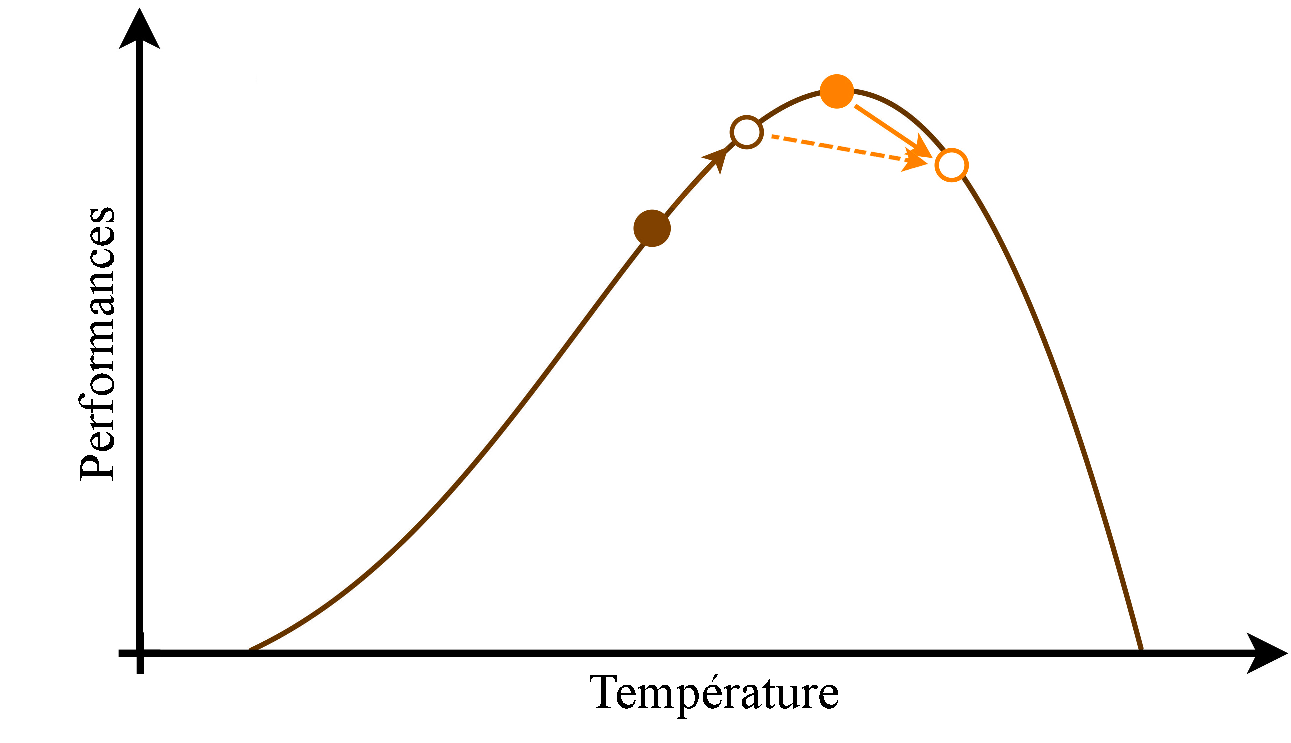
\includegraphics[width=0.66\textwidth]{1_CorpsDeThese/EA/Fig/ThermalCurve.pdf}
\caption[\lofimage{1_CorpsDeThese/EA/Fig/ThermalCurve.pdf}
Performance théorique en fonction de la température]{Performance théorique en
fonction de la température. D'après \textcites{ohlberger2013a}, Figure 1. Un
réchauffement du climat améliore les performances d'un individu qui vit dans
des conditions sous optimales si le changement est de petite amplitude (flèche
marron). Si l'individu est à l'optimum (point orange plein), le réchauffement
lui fait diminuer ses performances (flèche orange pleine). Si le changement est
de trop grande amplitude, les performances diminuent également (point marron
vide, flèche orange pointillée)}
\label{Fig:EA1}
\end{figure}

Cette sensibilité asymétrique à la température se répercute ensuite au niveau
de l'individu dans son ensemble, et en particulier sur son taux de croissance.
Ainsi, pour un individu vivant à une température sous-optimale, une augmentation
de température sera bénéfique alors qu'elle sera néfaste pour un individu vivant
déjà à sa température optimale. De même, si l'amplitude de l'augmentation est
trop importante, la température peut dépasser l'optimum et le réchauffement a
alors un effet néfaste . Ceci est illustré par la Figure
\ref{Fig:EA1}, d'après \textcites{ohlberger2013a}. Cependant, les individus sont
souvent capable d'adapter leur sensibilité à la température par plasticité
phénotypique. Ces réponses plastiques peuvent alors différer suivant la
fréquence et la longueur des changements de température
\autocites{angilletta2009a, huey1999a}.

Lorsque les températures subies sont contenus dans des valeurs non
extrêmes, permettant à un individu de se développer sans provoquer la diminution
du taux de croissance, la plupart des ectothermes suivent alors règle
taille--température déjà énoncée \autocite{atkinson1994a}. Ainsi, au cours du
développement, une plus forte température entraîne une augmentation du taux de
croissance mais une diminution de la taille adulte (Figure \ref{Fig:EA2}). On
observe donc une modification de la taille à un âge ou un stade donné avec la température (par
exemple la taille à maturité). Le suivi de ces modification permet de
déterminer précisément la norme de réaction à la température et la réponse d'un
organisme à son changement.

\begin{figure}[!ht] % Figure 1 
\centering
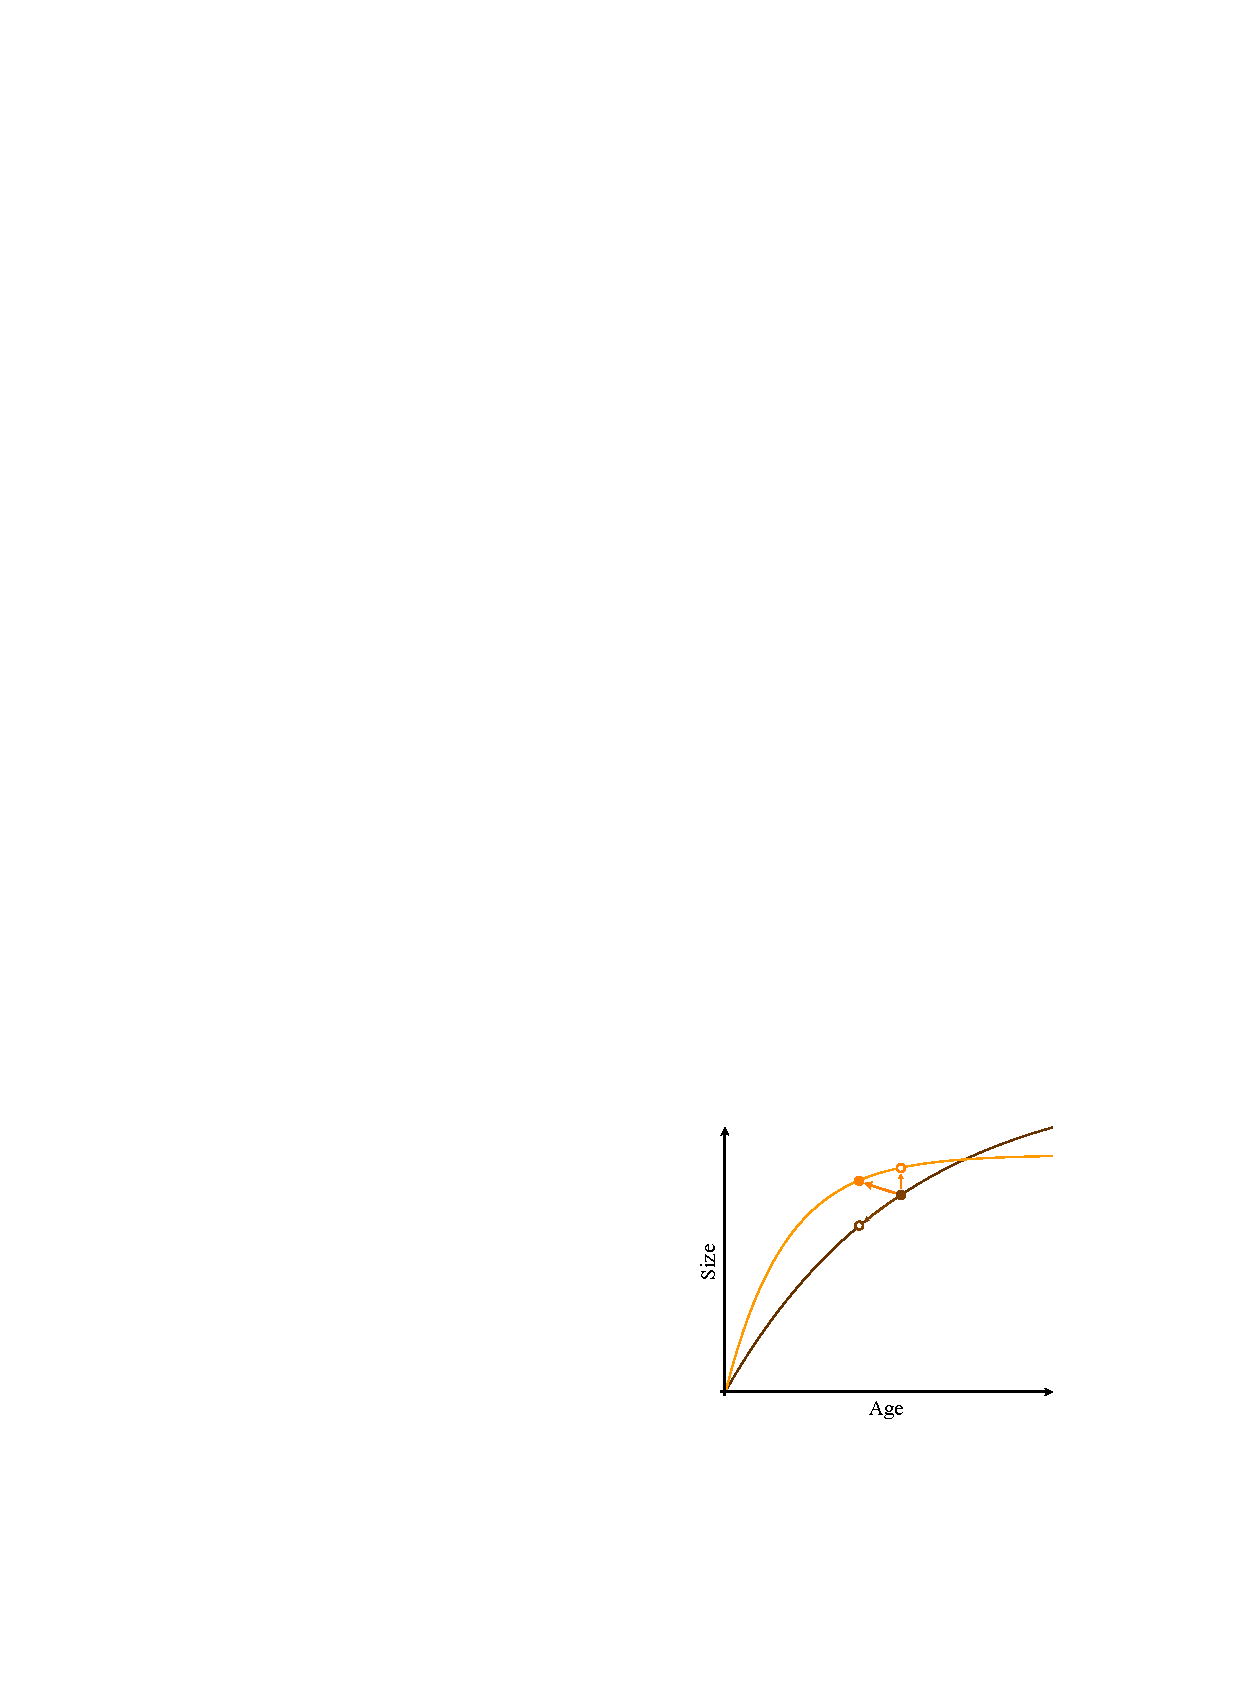
\includegraphics[width=0.5\textwidth]{1_CorpsDeThese/EA/Fig/ThermalNorm}
\caption[\lofimage{1_CorpsDeThese/EA/Fig/ThermalNorm}
Norme de réaction à la température]{Norme de réaction théorique à la
température \autocites[Figure 2]{ohlberger2013a}. Lors d'un changement de
température, le changement de taille à un âge donné (point orange plein) dépend
de l'importance relative de l'accélération de la croissance corporelle (point
orange vide), et de l'accélération du développement (point marron vide).}
\label{Fig:EA2}
\end{figure}

\subsection{Température et dynamique des populations}

La taille corporelle des individus et sa distribution étant un élément essentiel
dans la dynamique des populations, les variations de taille corporelle avec la
température ont des conséquences sur les dynamiques des populations et des
communautés. 

En effet, la température de l'environnement peut provoquer un changement de la
taille moyenne et de la structure d'une population. On retient en particulier
deux changements possibles : (i) la diminution de la taille à un âge donné avec
l'augmentation de la température (``size-at-age shift'') ; et (ii) le
changement de l'abondance relative des différents stades ou âges présents dans
la population (``structure shift''). Ces changements de structures sont causés
par l'intermédiaire de la croissance densité-dépendante, de la survie
taille-dépendante, de la compétition asymétrique entre les différentes
classes de taille et de la prédation taille-spécifique. Ces changements de
structures au niveau population peuvent ensuite se répercuter au niveau de la
communauté en affectant l'abondance relative de ses différentes espèces et son
organisation trophique. 

De plus, la température interagit fortement avec les mécanismes de densité
dépendance. Ainsi, il a par exemple été montré que le taux de croissance d'une
population peut augmenter avec la température si la population est présente en
faible densité, et à l'inverse diminuer avec la température si la population est
trop dense \autocites[chez le saumon royal][]{crozier2010a}. Dans le même
ordre d'idées, l'étude des registres de pêche du saumon d'atlantique a montré
qu'une température plus chaude était associée à des individus de grande taille si la
densité de la population était faible et l'inverse en climat froid
\autocites{huusko2012a}. 

La densité dépendance étant notamment lié à la compétition pour l'accès aux
ressources, qui elle-même dépend de la taille corporelle, l'augmentation de la
température peut provoquer une diminution de la taille moyenne dans une
population en favorisant des individus plus petits, plus compétitifs dans la
gestion de l'énergie s'il y a peu d'interférence
\autocites{persson1998a,ohlberger2012a}. Si la compétition par interférence est
forte, et une grande taille corporelle fourni un avantage compétitif conséquent,
l'effet de la température sur la compétition devient alors plus difficile à
prédire.

Enfin, la température peut avoir des effets différentiels suivant le stade ou
l'âge des individus. En effet, il a été suggéré que des individus juvéniles
survivent plus facilement à un réchauffement que des individus plus grands ou
plus vieux \autocites{peck2009a}. Une élévation de la température a donc des
effets différents suivant l'âge, le stade et la taille des individus, ce qui se
répercute sur la distribution de la taille dans la population, impactant
fortement sa dynamique. Ces changement de dynamique d'une population se
répercutent alors en cascade sur les communautés dont elles font partie, avec
des issues encore difficiles à prévoir. 


\section{Problématiques}	

\chapter{Le collembole, un modèle d'étude en écologie}
\section{Biologie}
\section{Cycle de vie}
\section{Conditions d’élevage}
\section{Méthodes de mesures et comptage (phenotypage populationnel haut débit)}
\section{Méthode de représentation graphique}


\selectlanguage{french}
\partimage[width=\textwidth]{FigParts/writing2}
\part{Résumé des travaux de thèse}


%% Chaque section est un résumé en français d'un papier présent dans les annexes.

\chapter{Accès à la ressource taille dépendant et compétition par interférence :
Analyse de séries temporelles longues de populations de collemboles \textit{Folsomia candida}}
\chaptermark{Analyse de séries temporelles structurées}
\label{chap:sp}

\vspace{5cm}

\lettrine[lines=3]{A}{ujourd'hui}, les conséquences de la compétition par
interférence sur les populations physiologiquement structurées, et plus
particulièrement les populations structurées en taille, restent assez peu
explorées. Nous présenterons dans ce chapitre les résultats d'une étude
expérimentale au cours de la quelle nous avons suivi 28 populations de
collemboles \textit{Folsomia candida} pendant $800$ à $1200$ jours. Cette étude
nous a permis d'en apprendre d'avantage sur le rôle que joue la structure des
populations à un instant donné sur la détermination de sa dynamique. Durant
cette étude, nous avons dénombré et mesuré la structure détaillée de $12$
populations du clone TO et $16$ populations du clone HA. Nous avons ensuite
réalisé une analyse qualitative et quantitative des séries temporelles obtenues
afin de relier les états (les structures) passés et présents de chaque
population avec sa dynamique future.
En particulier, cette étude nous a permis de mieux comprendre le rôle essentiel
que joue la présence d'individus de grande taille dans la régulation de la
dynamique des populations et de leur structure.

Les travaux présentés dans ce chapitre sont en cours d'écriture pour
publication, et peuvent être retrouvés dans l'Annexe \ref{Ann:SP}.

\section{Éléments de méthodologie}

\subsection{Conditions d'élevage et mesures des populations}

Nous avons élevé 28 populations de deux clones de
collemboles \textit{Folsomia candida} dans les conditions décrites dans le
Chapitre \ref{chap:method}: $12$ populations du clone TO et $16$
populations du clone HA. Pour chaque population les mesures de nombre
d'individus et de structure en taille des populations ont été réalisées toutes
les unes à deux semaines en suivant la méthode automatisée décrite dans le
Chapitre \ref{chap:method}, Section \ref{sec:bpsensor}.

\subsection{Analyse qualitative des séries temporelles}

Nous nous sommes d'abord intéressés aux dynamiques sur le long
terme de la structure des populations. Nous avons étudié de manière
qualitative ces dynamiques en traçant les séries temporelles structurées sur des
diagrammes structure-temps afin de faire ressortir le maximum d'information sur
la dynamique de la structure.
Nous avons alors séparé notre analyse en deux temps.

\subsubsection{Etat de la population}

Dans un premier temps, nous avons regardé la structure en taille des populations
de manière globale afin de repérer les structures caractéristiques que l'on
pouvait observer, sans considérer les dynamiques de court terme. Nous décrivons
alors plusieurs structures typiques différentes suivant le clone considéré et le
niveau de densité de la population.

\subsubsection{Dynamique de la structure de la population}

Dans un second temps, nous nous sommes attachés à décrire les dynamiques
temporaires que l'on peut observer sur les diagrammes structure-temps. Nous
avons essayé de déterminer des motifs dynamiques que l'on pouvait rattacher à
certains types de structures de populations, telles que celles décrites au
par avant, ou à certains changements dans ces structures.

\subsection{Analyse quantitative des dynamique de populations}

Suite à la description qualitative des dynamiques, nous avons réalisé une
analyse quantitative des structures observées et de leur dynamique. 

\subsubsection{Analyse en composante principale}

A chaque date de mesure, les données comprennent le nombre d'individus et pour
chaque individu sa longueur corporelle. Nous avons regroupé les données de
l'ensemble des populations à toutes les dates de mesures et nous avons
discrétisé la taille en classes de $0.1mm$ de $0$ à $3mm$. Nous obtenons ainsi
un tableau de données de $3341$ lignes (une ligne par classe de taille par date
par population) et $30$ colonnes. Chacune des colonne peut alors être considéré
comme un vecteurs de base dans l'espace à $30$ dimensions qui constitue l'espace
des structures de nos populations, et chaque ligne comme une observation dans
cet espace. Étant donnée la différence d'ordre de grandeur dans les nombres
d'individus entre juvéniles et adultes, nous avons utilisé le logarithme des
nombre d'individus dans chacune des classes de taille.

En considérant que chaque ligne est indépendante des autres, nous avons alors
réalisé une analyse en composantes principales (ACP) de nos données compilées.
Cela nous a permis d'extraire les quelques premières composantes et les vecteurs
et valeurs propres correspondantes. Ainsi, en ne conservant que peu de
composantes, on obtient une représentation condensée à quelques dimensions
(deux ou trois dans notre cas) des données de départ. Nous avons alors projeté
chacune des dynamiques de la structure des populations sur les deux première
composantes de la décomposition. Un point dans l'espace à deux dimension
représente alors une condensation de la structure d'une population à une date
donnée. 

\subsubsection{Regroupement non hiérarchique et projection sur les premières
composantes}

Parallèlement à l'ACP, nous avons effectué un regroupement non hiérarchique par
l'algorithme des ``k-means'' de nos données compilées. Ceci permet de regrouper
ensemble les structures de populations qui partagent des caractéristiques
communes, indépendemment de la date de mesure, du clone ou de la dynamique de la
population. Ainsi, nous avons pu déterminer quatre groupes cohérents de
structures de populations et identifier leur caractéristiques précises. Une fois
projetés sur les deux premières composantes de l'ACP, les groupes obtenus
délimentent quatre régions distinctes du plans, confirmant ainsi la cohérence du
regroupement. 
 
\subsubsection{Dynamique des populations}

La visualisation des données sur le plan des deux premières composantes de l'ACP
et le regroupement en quatre types de structures permettent de représenter la
dynamique de la structure des populations comme une trajectoire dans ce plan.
Cette trajectoire permet alors une analyse objective des dynamiques en
déterminant par exemple des temps de résidence dans chacune des structures type,
les nombres de transitions entre différentes structures types et la direction de
ces transitions. 

\section{Résultats}

Nous présenterons ici l'analyse détaillée de quatre populations, deux du clone
TO et deux du clone HA, ainsi que les résultats de l'analyse de l'ensemble des
populations. L'analyse graphique de chacune des populations est disponible à la
fin de l'article en Annexe \ref{Ann:SP} page \pageref{Ann:SP}. 

\subsection{Etude descriptive}

\subsubsection{Etats des populations}

La première partie de cette étude concerne une description qualitative des
périodes stables de la structure des populations (Figure \ref{fig:SP1}). On
appellera état des populations ces structures caractéristiques que l'on retrouve dans les
différentes populations. 

\begin{figure}[!ht]
\begin{center}
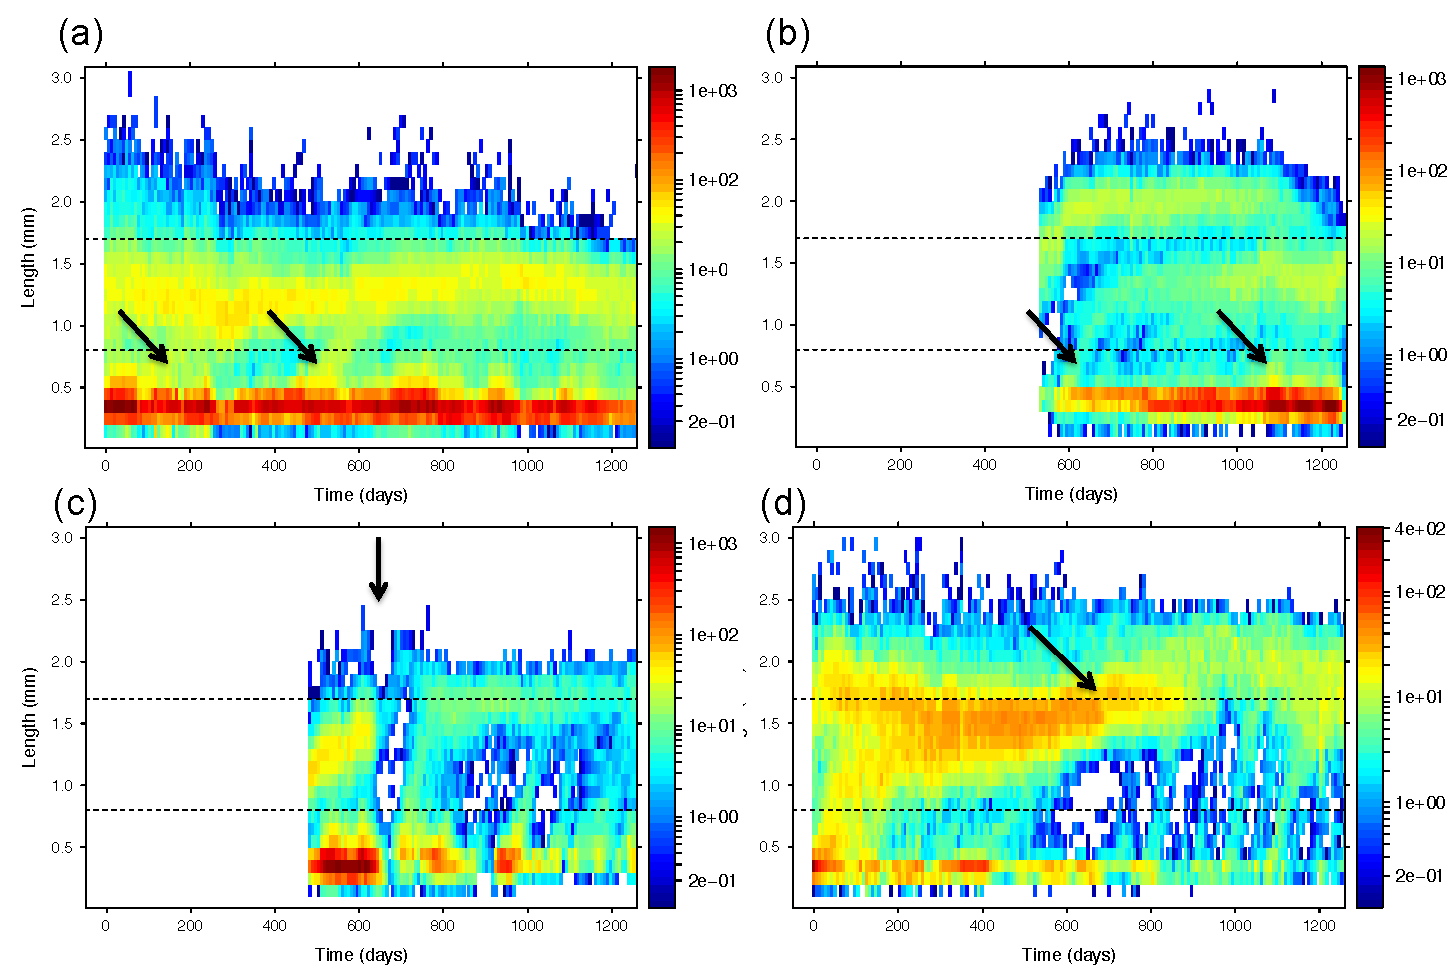
\includegraphics[width=0.95\textwidth]{1_CorpsDeThese/Resumes/Fig/SP01}
\caption[\lofimage{1_CorpsDeThese/Resumes/Fig/SP01}Dynamiques de la
structure de 4 populations]{Dynamique de la structure de 4 populations de
collembole. (a) Clone TO, réplicat 3. (b) Clone HA, réplicat 15. (c) Clone TO,
replicat 11. (d) Clone HA, réplicat 4. Les flèches noires en (a) et (b) montrent
des périodes de recrutement. Les flèches noires de (c) et (d) montrent des
événements conduisant à un nouveau recrutement, respectivement une catastrophe
(c) et la sénescence de la cohorte d'adultes (d).}
\label{fig:SP1}
\end{center}
\end{figure}

Les Figures \ref{fig:SP1}a et b montrent deux populations aux structures
relativement stables, mais dont la distribution en taille diffère. Dans le
premier cas, on constate que la distribution de la taille est fortement
bi-modale avec un groupe de juvéniles très dense ($>700$ individus de moins de
$0.5mm$) et un groupe de d'adultes ($<250$ individus de plus de $0.8mm$), mais
très peu d'individus de taille intermédiaire. Dans le second cas, on retrouve
ces deux même groupes pendant la totalité de la série temporelle, mais avec une
longue période pendant la quelle un troisième groupe de très grands adultes
subsiste ($>1.2mm$). Ces distributions multi-modales sont universelles dans les
populations étudiées. La plupart des populations ont une structure bi-modale,
plus ou moins stable dans le temps, tandis que certaines populations montrent
une structure tri-modale, exclusivement chez le clone HA. Le clone HA est donc
cable de produire des adultes de très grand taille à la survie très longue, ce
que TO est incapable de faire.

\subsubsection{Dynamique de la structure}

Dans un second temps, on s'intéresse maintenant aux événements dynamiques rapide
à l'échelle des séries temporelles. En effet, même si la structure peut être
relativement stable (Figure \ref{fig:SP1}a et b), on peut observer que des
processus dynamiques sont à l'oeuvre.
 
\paragraph{Recrutement de cohortes}

Un premier processus remarquable est le recrutement de juvéniles dans les
classes d'adultes (flèches sur les Figures \ref{fig:SP1}a et b). Ces périodes de
recrutement  durent entre quelques dizaines et quelques centaines de jours, et
se retrouve plus ou moins fréquemment, mais dans l'ensemble des populations
étudiées. On constate sur la Figure \ref{fig:SP1}b que ces recrutements
n'atteignent jamais la cohorte d'adultes les plus grands.
Ceci est vrai pour toutes les populations dans les quelles un groupe d'adultes
de très grande taille subsiste. Lorsque ces individus géants sont présents dans
une populations, il semble alors impossible pour les autres de grandir jusqu'à
ces tailles.

Ces périodes de recrutement permettent également d'estimer des taux de
croissance corporelle en fonction des conditions de la population (clone et
densité dans les différentes classes) en mesurant la pente de la cohorte qui
recrute. Ainsi, le taux de croissance de la cohorte marquée par la seconde
flèche de la Figure \ref{fig:SP1}a est d'environ $5\cdot 10^{-3}mm/j$, soit
$1mm$ tous les 200 jours. L'étude de ces taux de croissance en fonction de la
densité et des conditions de température fera l'objet du Chapitre \ref{chap:fip}
et de l'Annexe \ref{Ann:fip}.

Ces périodes de recrutement surviennent parfois à la suite d'événement
catastrophiques. On constate sur la Figure \ref{fig:SP1}c (flèche) que c'est
après la disparition brutale et quasi-totale des adultes que survient un des
plus gros recrutements d'individus de la série temporelle. Ceci se retrouve
également sur d'autre population (voir Table \ref{tab:SP}). Ainsi, la
disparition brutale des adultes de la population déclenche le recrutement de
nouveaux individus chez les adultes. 

Enfin, le recrutement de nouvelle cohortes de juvéniles peut également
intervenir après le déclin naturel du groupe d'adultes, soit chez le groupe de
géants (Figure \ref{fig:SP1}b, seconde flèche), soit le seul groupe présent
(Figure \ref{fig:SP1}d, flèche). On constate par exemple dans le second cas que
pendant une très longue période la population est composée de quelques jeunes et
d'une très large cohorte d'adulte, avec très peu de recrutement de nouveaux
adultes. Ce groupe d'adulte décline au cours du temps, et lorsqu'il a
suffisamment diminué en densité (aux environs de $800$ jours, flèche), des
recrutements de jeunes commencent à survenir. Ceci confirme le rôle des
adultes de plus grande taille dans le contrôle de la dynamique de la structure
et le renouvellement des populations. 

\paragraph{Plasticité de la taille adulte}

L'étude de ces séries temporelles révèle également des ajustements de la taille
des adultes au cours des différents événements décrits précédemment. Tout
d'abord, suivant les conditions démographiques, les cohortes d'adultes se
stabilisent à différentes tailles. Les populations montrées en exemple sur la
Figure \ref{fig:SP1} montrent chacune une taille d'équilibre différente. En
particulier, la taille adulte a tendance à être plus grande quand la densité
de la population est plus faible. Ce point fera également l'objet d'une étude
approfondie dans le Chapitre \ref{chap:fip}.

De plus, les individus sont capables d'ajuster rapidement leur taille corporelle
en fonction des changements de conditions environnementales et démographiques.
Après la chute catastrophique de la cohorte d'adulte montrée Figure
\ref{fig:SP1}c, les adultes survivants reprennent une croissance très rapide sur
une courte durée (augmentation de près de $40\%$ de leur taille corporelle en
quelques semaines).
De même dans le cas de la sénescence des adultes (Figure \ref{fig:SP1}d), où les
adultes restant grandissent de $1.7mm$ à près de $2.2mm$.

De façon plus étonnante, les adultes sont également capables de diminuer leur
taille corporelle. Par exemple au cours des $200$ premiers jours sur la Figure
\ref{fig:SP1}d où la taille des adultes diminue pendant qu'une grande cohorte de
juvéniles atteint la maturité. Ces rétrécissements des adultes ont été observées
dans d'autres populations (HA réplicats 1 à 3, TO réplicats 5 et 9 par exemple).
La plasticité de la taille adulte des collemboles est décrite et étudiée par
\textcites{mallard2013b} dans ses travaux de thèse.

La Table \ref{tab:SP} résume les dates où les différents événements décrits ont
été observés dans les populations étudiées. 

{\tiny
\begin{longtable}{
	p{\dimexpr.12\linewidth-2\tabcolsep-1.3333\arrayrulewidth}% column 1
 	p{\dimexpr.128\linewidth-2\tabcolsep-1.3333\arrayrulewidth}
 	p{\dimexpr.128\linewidth-2\tabcolsep-1.3333\arrayrulewidth}% column 1
 	p{\dimexpr.128\linewidth-2\tabcolsep-1.3333\arrayrulewidth}
 	p{\dimexpr.12\linewidth-2\tabcolsep-1.3333\arrayrulewidth}% column 1
 	p{\dimexpr.12\linewidth-2\tabcolsep-1.3333\arrayrulewidth}
 	p{\dimexpr.126\linewidth-2\tabcolsep-1.3333\arrayrulewidth}% column 1
 	p{\dimexpr.126\linewidth-2\tabcolsep-1.3333\arrayrulewidth}}
 	
 	\caption{Dates d'observations des états et dynamiques
 	décrites. Les nombres correspondent aux dates en jours ou aux
 	intervalles pendant les quels les événements ont été
 	observés.}\label{tab:SP}\\
 	\hline
 	\endhead
 	
\hline
\endfoot

Populations & Structure Trimodale & Longue période sans recrutement &
Recrutement fréquent & Evénement catastrophique & Senescence de la cohorte adulte &
Croissance adulte d'ajustement & Rétrécissement adulte d'ajustement \\
\hline\\
HA r1 & - 			& - 		& - 		& - 	& 500  & 500-650  & 650-750  \\
HA r2 & - 			& - 		& - 		& - 	& 800  & 650-900  & - 		 \\
HA r3 & - 			& - 		& - 		& - 	& 800  & 900-1000 & 1000-1250\\
HA r4 & - 			& - 		& - 		& - 	& 800  & 600-1000 & -        \\
HA r5 & 600-1000 	& - 		& - 		& - 	& 1000 & - 		  & - \\
HA r6 & - 			& 800-1250 	& - 		& - 	& -    & - 		  & - \\
HA r7 & 700-1100 	& - 		& - 		& - 	& 1000 & - 		  & - \\
HA r8 & 600-1000 	& - 		& - 		& - 	& 950  & - 		  & - \\
HA r9 & 700-1200 	& 700-1100 	& - 		& - 	& -    & - 		  & - \\
HA 10 & 600-900 	& - 		& - 		& - 	& 900  & - 		  & - \\
HA 11 & 600-1100 	& 700-1250 	& - 		& - 	& 1100 & - 		  & - \\
HA 12 & 600-900 	& - 		& 600-1250 	& - 	& 1000 & - 		  & - \\
HA 13 & 600-1100 	& - 		& 600-1250 	& - 	& 1100 & - 		  & - \\
HA 14 & 600-1100 	& 600-1000 	& - 		& - 	& 1100 & - 		  & - \\
HA 15 & 600-1100 	& - 		& 600-1250 	& - 	& 1100 & - 		  & - \\
HA 16 & 600-1200 	& - 		& - 		& - 	& 1200 & - 		  & - \\
TO r1 & - 			& 400-600 	& 0-400 	& - 	& 400  & 400-600  & -\\
	  &				& 700-1000	& 1000-1250 & 		&	   &		  &\\
TO r2 & - 			& 500-750 	& 0-450 	& - 	& 400  & 500-700  & - \\
	  & 			& 			& 1000-1250 &		&	   &		  &\\
TO r3 & - 			& 600-1250 	& - 		& - 	& -    & - 		  & 0-200\\
TO r4 & - 			& - 		& 0-1250	& - 	& 400  & - 		  & 700-1000\\
TO r5 & - 			& - 		& - 		& 900 	& -    & 900-1000 & 500-700\\
TO r6 & - 			& 600-950 	& - 		& 950 	& -    & 950-1000 & -\\
TO r7 & - 			& - 		& 500-1250 	& - 	& -    & - 		  & -\\
TO r8 & - 			& 600-800 	& 800-1250 	& - 	& 1000 & 1000-1100& -\\
TO r9 & - 			& 600-1000 	& - 		& - 	& 950  & 900-1000 & 500-600\\
TO 11 & - 			& - 		& 700-1250 	& 650 	& -    & 650-750  & -\\
TO 12 & - 			& - 		& - 		& 750 	& -    & 750-850  & -\\
TO 13 & - 			& 500-800 	& 800-1250 	& 800 	& -    & - 		  & -\\

\end{longtable}
}

\subsection{Analyse quantitative des dynamiques}

\subsubsection{Composantes principales}

\begin{figure}[!ht]
\begin{center}
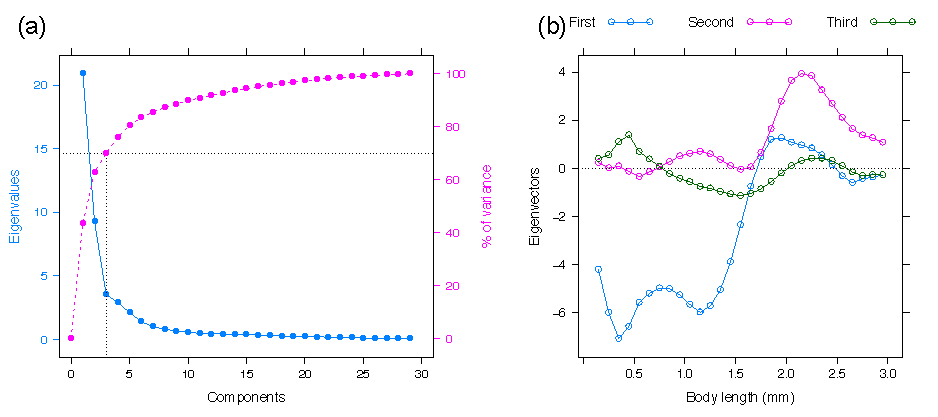
\includegraphics[width=0.95\textwidth]{1_CorpsDeThese/Resumes/Fig/SP02}
\caption[\lofimage{1_CorpsDeThese/Resumes/Fig/SP02}Composantes
principales]{(a) Scree plot de l'ACP. La ligne bleue pleine donne les valeurs
propres, la ligne pointillée donne le pourcentage cumulé de variance expliquée.
(b) Coordonnées des trois premiers vecteurs propres.}
\label{fig:SP2}
\end{center}
\end{figure}

La Figure \ref{fig:SP2}a représente les valeurs propres de l'ACP et le
pourcentage cumulé de variance expliquée. On observe une cassure nette après la
troisième composante, les trois premières composantes expliquant $70\%$ de la
variance totale. Cela montre que les trois premières composantes permettent
d'expliquer l'essentiel des variations entre les structures dans nos différentes
populations. La Figure \ref{fig:SP2}b montre que ces trois composantes
expliquent des variations sur l'ensemble de notre espace de départ sans classe
de taille non expliquée..
En particulier, la première composante expliquant $43\%$ de la variance
correspond essentiellement aux variations dans les individus de moins de
$1.5mm$. La seconde composante quand à elle, qui représente $20\%$ de la
variance explique une partie des variations des petits adultes ($0.8$ à
$1.3mm$), et principalement au niveau des individus de plus de $1.6mm$. La troisième
composante enfin permet de distinguer entre les individus de taille
intermédiaire ($0.8$ à $1.9mm$) et les petits individus ($<0.8mm$). Ces trois
composantes permettent de définir plusieurs groupes de classes de taille sans a
priori: (i) les juvéniles ($<0.6mm$), négatifs sur le premier axe et positif sur
le troisième; (ii) les petits adultes (entre $0.6$ et $1.2mm$) positif sur le
second axe, négatif sur les autres; (iii) les adultes intermédiaires ($1.2$ à
$1.9mm$) négatifs sur le troisième axe; et (iv) les grands adultes ($>1.9mm$),
positifs sur le second axe. Ces groupes recoupent bien la description
qualitative des diagrammes mais sans a priori sur les limites entre groupes.

Les deux premières composantes représentant $63\%$ de la variance, nous ne
conserveront pas la troisième composante dans la suite de l'étude. Cela nous
permettra une représentation graphique simplifiée des structures des populations
dans le plan des deux premières composantes. 

\subsubsection{Groupement non hiérarchique}

En utilisant l'algorithme des ``k-means'', nous avons regroupé les structures
qui partageaient des caractéristiques communes en quatre groupes. En traçant ces
structures ensemble, nous avons pu déterminer quatre grandes structures typiques
de populations expérimentales (Figure \ref{fig:SP3a}): (i) une
structure avec beaucoup de juvéniles et des adultes de petite taille (type $1$);
(ii) une structure avec des adultes de taille intermédiaire (type $2$); (iii)
une structure avec moins de juvéniles et des adultes de grande taille (type
$3$); et (iv) une structure trimodale avec des juvéniles, des petits et des
grands adultes (type $4$).

\begin{figure}[!ht]
\begin{center}
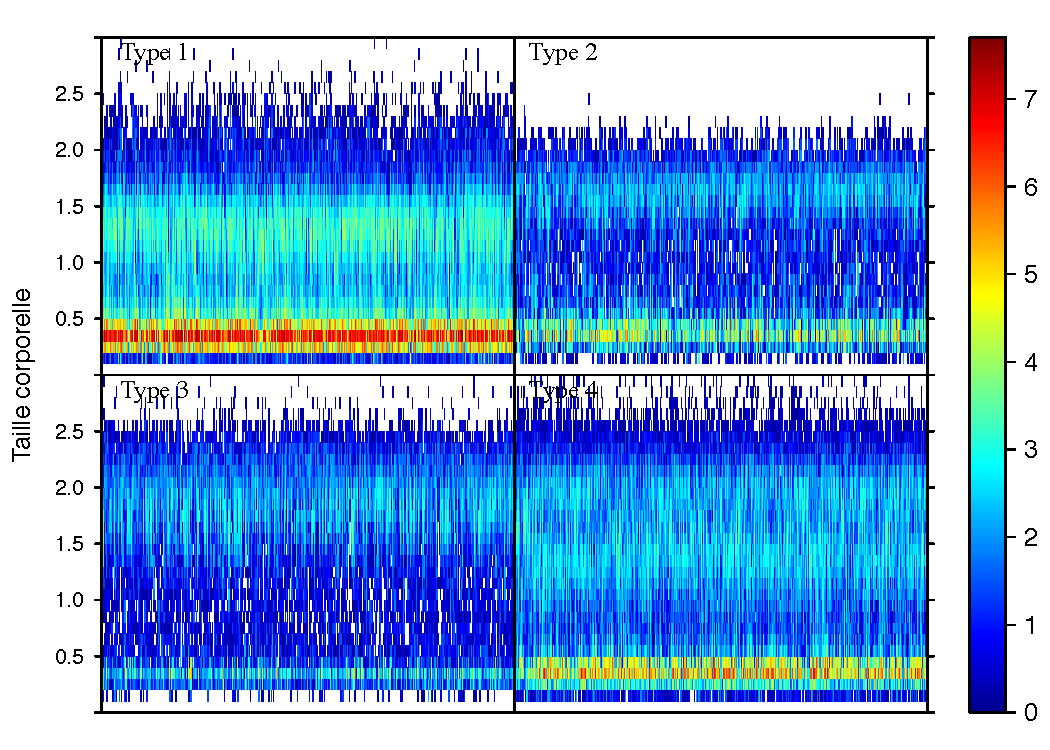
\includegraphics[width=0.95\textwidth]{1_CorpsDeThese/Resumes/Fig/SP02b}
\caption[\lofimage{1_CorpsDeThese/Resumes/Fig/SP02b}Quatres grands
types de structures]{Structures caractéristiques des quatre grands types de
structure identifiés.}
\label{fig:SP3a}
\end{center}
\end{figure}

En projetant la structure de chacune des populations à chaque date de mesure
sur les deux premières composantes de l'ACP, et en séparant les points en
fonction du type de structure auxquels ils appartiennent, on constate que la
séparation en quatre groupes reste remarquablement cohérente dans l'espace
réduit à deux dimensions (Figure \ref{fig:SP3}), et délimitent quatre régions
distinctes du plan.

\begin{figure}[!ht]
\begin{center}
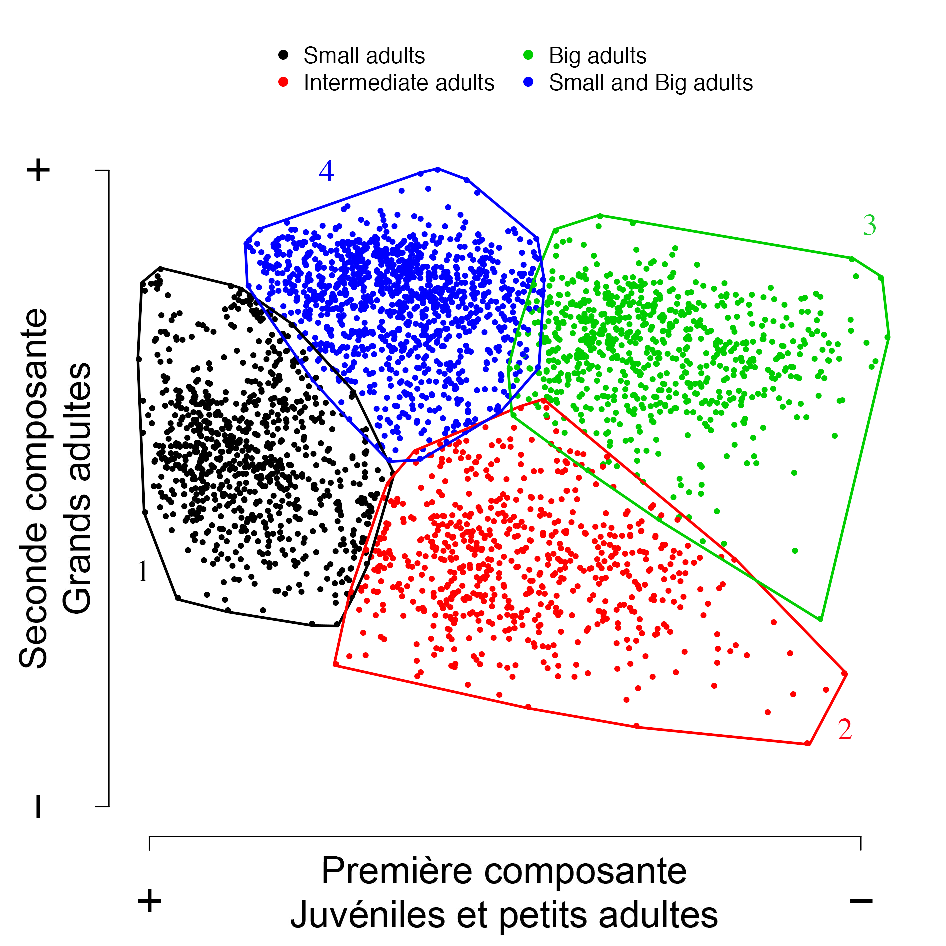
\includegraphics[width=0.75\textwidth]{1_CorpsDeThese/Resumes/Fig/SP03b}
\caption[\lofimage{1_CorpsDeThese/Resumes/Fig/SP03b}Projection des données
sur les deux premières composantes]{Projection des structures sur les deux
premières composantes de l'ACP et groupement en 4 types de structure. Les
domaines délimités seront reportés sur les trajectoires temporelles dans le
plan des deux premières composantes.}
\label{fig:SP3}
\end{center}
\end{figure}

Cette représentation permet une classification objective de la structure d'une
population à un temps donné dans un des quatre type de structure, ainsi que
d'observer la trajectoire temporelle dans le plan des deux premières composantes
de l'ACP et donc sa dynamique entre les différentes structures caractéristiques. 

\subsubsection{Trajectoires dans le plan des composantes}

\begin{figure}[!ht]
\begin{center}
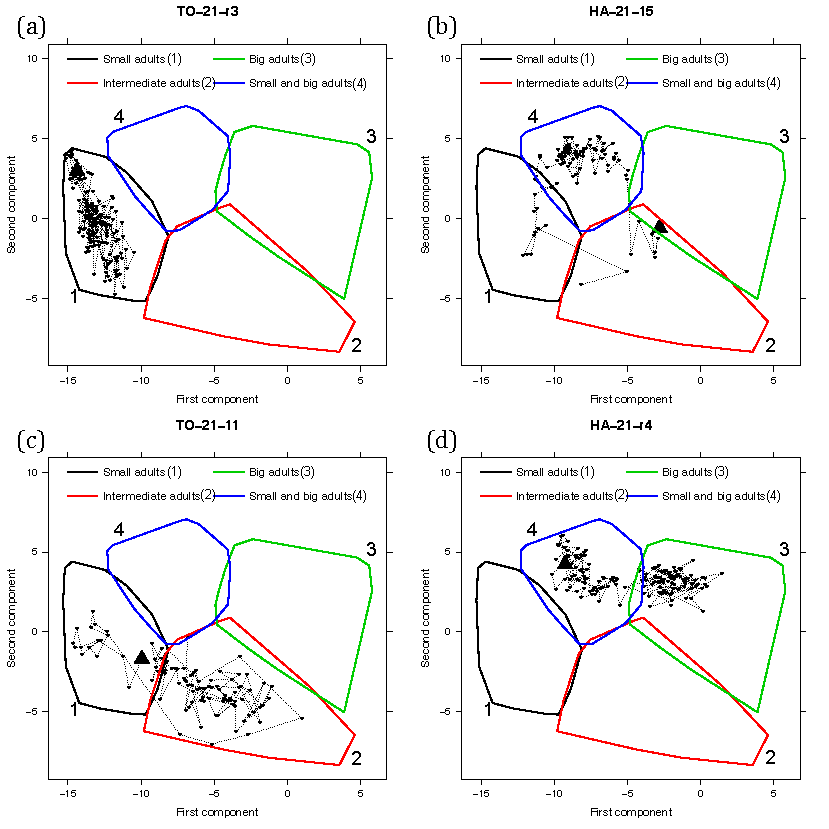
\includegraphics[width=0.95\textwidth]{1_CorpsDeThese/Resumes/Fig/SP04}
\caption[\lofimage{1_CorpsDeThese/Resumes/Fig/SP04}Trajectoires des
popualtions exemple dans le plan des composantes]{Trajectoires des
populations exemples dans le plan des composantes. Les lignes colorées et
numérotées représentes les quatre grands types de structure issus de la
classification non hiérarchique. Chaque points est une mesure de structure à
une date donnée. Le triangle représente le début de la trajectoire. Les lignes
pointillées relient chronologiquement les points.}
\label{fig:SP4}
\end{center}
\end{figure}

La Figure \ref{fig:SP4} montre les mêmes populations que sur les diagrammes
structure-temps de la Figure \ref{fig:SP1}, en projetant les structures dans le
plan des deux premières composantes. Cette représentation permet de confirmer
numériquement que la population TO 3 (Figures \ref{fig:SP1}a et \ref{fig:SP4}a)
reste tout le temps dans une structure de type 1 alors que la population TO 11
(Figures \ref{fig:SP1}c et \ref{fig:SP4}c) débute dans une structure de type 1
mais converge finalement vers une structure de type 2 avec moins de juvéniles et
des adultes plus grands. De même pour les populations HA  (Figures
\ref{fig:SP1}bd et \ref{fig:SP4}bd) qui restent toutes les deux dans une
configuration de type 4 trimodale avant de basculer, l'une vers une structure de
type 2 avec des adultes petits à intermédiaires (panels b), l'autre vers une
structure de type 3 avec des grands adultes (panels d).

\subsubsection{Stabilité des structures et transitions}

L'ACP et la projection des dynamiques sur les deux premières composantes
permettent de mesurer des temps de résidence dans chacun des 4 types de
structure, et des transitions entre les grands types. Par exemple, alors que la
population TO 3 (Figures \ref{fig:SP1}a et \ref{fig:SP4}a) est très stable et
passe 1200 jours dans le même type de structure, les autres populations ont
tendance avoir des transitions entre plusieurs types de structures. En
particulier, la population HA 15 (panels b) a une phase transitoire d'une
cinquantaine de jours en type 2 avant de se stabiliser en type 4 pendant 550
jours, puis de revenir en type 2. En conduisant la même analyse sur chacune des
28 populations, nous pouvons alors étudier la distribution du temps passé dans
chacune des régions par chacun des clones. 

\begin{figure}[!ht]
\begin{center}
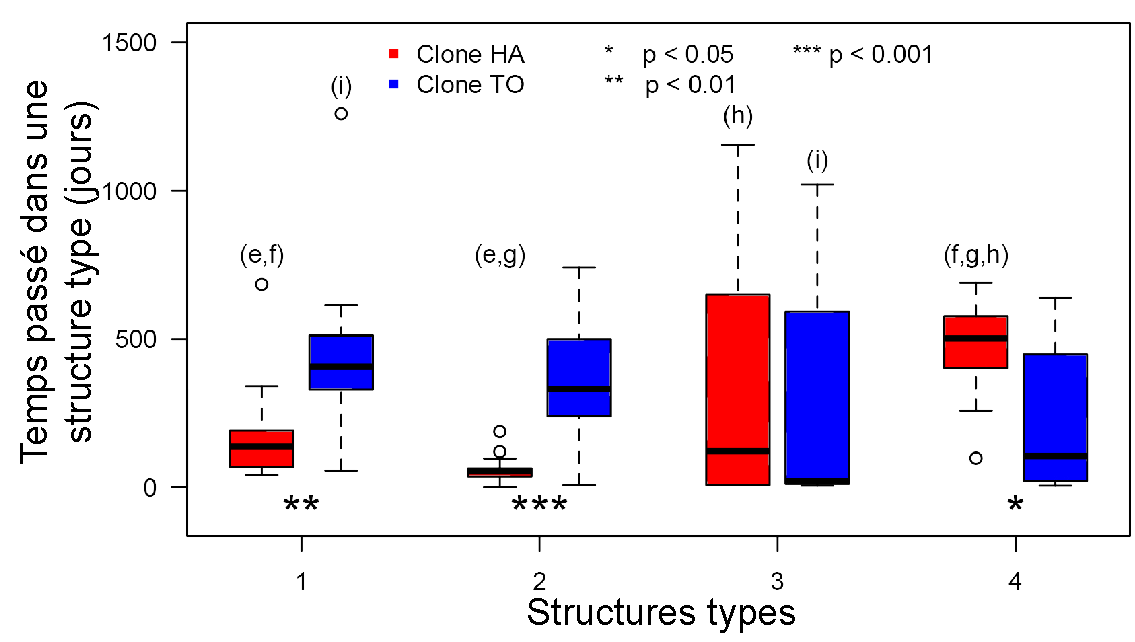
\includegraphics[width=0.95\textwidth]{1_CorpsDeThese/Resumes/Fig/SP05}
\caption[\lofimage{1_CorpsDeThese/Resumes/Fig/SP05}Temps de
résidence dans les structures types]{Temps passé dans chacun des types de
structure caractéristique suivant les clones. Les lettres montrent les
différences significatives dans les distributions (Tests de Kolmogorov-Smirnov
à deux échantillons: (e) D=0.54, p=0.02, (f) D=0.78, p=0.0003, (g) D=0.93,
p=3x10-6, (h) D=0.53, p=0.03, (i) D=0.67, p=0.04). Les étoiles montrent les
différences significatives entre clones dans un même type de structure.}
\label{fig:SP5}
\end{center}
\end{figure}

On constate alors que les différents types de structures ne sont pas tous aussi
stables (Figure \ref{fig:SP5}). Ainsi, bien que la variabilité soit très grande,
les temps de résidence les plus longs observés sont dans le type 3, avec des
adultes de grande taille.
Ces adultes de grande taille ont une très grande longévité et subissent peu de
compétition de la part des autres individus, ce qui a un effet stabilisant sur
la structure de la population. Cet effet est également visible pour les
structures trimodales (type 4) ou les temps de résidences sont également très
long. A l'opposé, les structures de types 2 sont les moins stables, en effet,
les adultes intermédiaires vont être soit exclus compétitivement par les plus
petits, ce qui fait revenir la population en type 1, soit plus fréquemment
continuer à grandir, ce qui fait basculer la population en type 3.

On constate également qu'il existe des différence marquées entre clones. Ainsi,
TO passe plus de temps dans les structures de type 1 et 2 où les adultes sont
plus petits et la densité de juvéniles est importante, alors que HA est plus
souvent dans une structure de type 3 ou 4 avec des adultes de très grande taille
et moins de juvéniles. Cela reflète des stratégies d'histoire de vie différentes
des clones TO et HA, le premier ayant tendance à privilégier la reproduction sur
la croissance, alors que le second privilégie la croissance sur la reproduction.

\section{Discussion}

\subsection{Conséquences des différences génétiques sur la dynamique des
populations}

Les différences de stratégies d'histoires de vie peuvent avoir un effet très
fort sur la dynamique des populations via notamment deux impactes. Le premier
est sur la réponse à la compétition, en effet les juvéniles sont plus compétitif
dans le cas de l'exploitation alors que les grands adultes sont supérieurs dans
le cas de l'interférence. Le second concerne la réponse à des changements de
températures puisqu'on a vu que ces derniers pouvaient affecter la taille
individuelle et les structures des populations. Les deux clones étudiés sont
connus pour leur stratégies différentes \autocites{tully2006a,tully2008a}, TO
étant très flexible dans son investissement reproducteur au détriment de sa
taille corporelle, alors que HA l'est moins mais atteint des plus
grandes tailles.

Ces différences affectent la dynamique de la structure des populations puisque
la faible flexibilité de HA et sa capacité à produire des adultes de grande
taille lui permettent d'atteindre des structures de type 3 voir 4 très
stables alors que TO reste dans des structures de type 1 ou 2. Une
fois établis, les adultes de grande taille dominent la population et empêchent
les autres individus de grandir monopolisant la ressource, ce qui amène
notamment à la stabilisation d'un groupe de petits adultes et des structures de
type 4 trimodales. Cela montre l'importance de connaître les stratégies
d'histoire de vie des espèces étudiées afin de comprendre correctement la
dynamique de leur structure et \textit{in fine} de prédire la dynamique de la
population dans son ensemble.

\subsubsection{Le rôle des conditions initiales}

Bien que la structure de type 4 semble très stable, il est intéressant de noter
qu'elle n'est visible qu'au début de certaines séries temporelles. En effet, ce
type de structure est très stable localement, mais n'est atteignable que dans
des conditions très particulières. Il est nécessaire: (i) que les individus
puissent grandir vite jusqu'à des très grandes tailles, ce qui est le cas
de HA mais pas de TO; et (ii) que le niveau de compétition soit à son minimum,
ce qui se traduit par une absence d'adulte dans la population, et une faible
densité de jeunes. Dans ces conditions, les jeunes présents vont alors grandir
jusqu'aux plus grandes tailles et commencer à se reproduire tout en monopolisant
la ressource, ce qui n'autorise les autres juvéniles à grandir que jusqu'à des
tailles intermédiaires. 

Les autres types de structures dépendent aussi des conditions initiales. Une
forte densité de juvéniles comme condition initiale d'une population conduira à
une structure de type 1 alors qu'une distribution relativement homogène en
densité moyenne conduira à une structure de type 2 chez TO et de type 3 chez HA.
L'importance des conditions initiales montre la coexistence des quatre
attracteurs quasi-stables de la structure des populations. De plus, les
transitions entre ces attracteurs sont généralement dues soit à un événement
catastrophique, soit à la sénescence des adultes de grande taille. 

Enfin, cette sensibilité aux conditions initiales montre l'importance de
considérer la structure dans l'étude de la dynamique des populations. En effet,
bien que le nombre d'individus globale puisse être le même, une structure
différente pourra mener à des dynamiques très différentes, ce
qui inclue la survie potentielle de la population. Cela va dans le sens des
résultats de \textcites{benton2005a} sur la dynamique de populations
d'acariens structurées en âge montrant que des séquences données de changements
environnementaux peuvent amener à des dynamiques très différentes en fonction de
détails des conditions initiales de la structure en âge et de la densité des
populations.

\subsubsection{La compétition par interférence}

Nous avons montré à plusieurs reprise le rôle déterminant que jouent les adultes
de grande taille dans la dynamique de nos populations. Si l'accès à la ressource
n'était régulé que par la compétition par exploitation, tous les individus
parviendraient à accéder à la ressource, et la théorie du budget énergétique
dynamique nous prédit que les grands individus seraient exclus par les plus
petits, plus efficaces dans leur gestion de l'énergie. Dans ces conditions, les
structures tendraient vers une majorité de juvéniles et des adultes qui ne
grandissent plus une fois la maturité atteinte. 

Or, nos dynamiques montrent clairement que les individus de grande taille
exercent une domination sur les populations: (i) certaines conditions permettent
l'émergence et le maintient à long terme de cohortes d'adultes géants; (ii) lors
de la disparition catastrophique d'une cohorte d'adultes, les juvéniles présents
commencent immédiatement à grandir; (iii) la sénescence d'une cohorte d'adulte
et sa disparition progressive se traduit aussi par une reprise de la croissance
des juvéniles; et (iv) des cohortes très dense d'adultes s'accompagnent
généralement de longues périodes sans recrutement. Ainsi, il semble que nos
populations soient régulées par la domination des adultes. Un mécanisme probable
permettant cette domination adulte serait la position privilégiée qu'ils
occupent dans l'accès à la ressource disponible, privant les plus petits
individus, les empêchant de grandir. Ceci est un mécanisme caractéristique de la
compétition par interférence. Lorsque le nombre d'adultes de grande taille
diminue, la pression de compétition est relâchée et les plus petits individus
parviennent de nouveau à accéder à la ressource et à se développer.


\section{En conclusion}

Cette étude montre ainsi que l'analyse de la dynamique temporelle de la
structure des populations permet d'accéder plus précisément aux mécanismes en
jeu dans leur régulation, tels que le rôle des stratégies individuelles
d'histoire de vie, ou le type d'interaction compétitive à l'oeuvre. Nous pensons
que cette étude est un exemple concret du fait qu'une population puisse être
contrôlée par ses adultes les plus grands, donnant lieu à des dynamiques
complexes qui dépendent directement des stratégies d'histoire de vie des
individus et des conditions environnementales, y compris la densité de
la population.
Modéliser le rôle de la compétition par interférence dans la dynamique des populations structurées, dans le cadre des modèles PSP, nous
permettra de confirmer son rôle essentiel dans la survie des
individus de grande taille, et dans l'émergence de dynamiques temporelles
impliquant des distributions de taille multi-modales (Chapitre
\ref{chap:amnat}).

De plus, il serait nécessaire de vérifier précisément le rôle joué par les
adultes, notamment pour confirmer leur domination dans l'accès aux ressources,
ce qui viendrait confirmer l'hypothèse de l'interférence comme mécanisme de
régulation des populations. Ceci fera l'objet d'une étude expérimentale
présentée dans le Chapitre \ref{chap:sm}.




\chapter[Interférence vs. exploitation et dynamique des populations
structurées][Interférence et populations structurées]{Interférence vs.
exploitation et dynamique des populations structurées}
\label{chap:amnat}

\vspace{2cm}
\begin{Spacing}{1}
\texttt{
Le Bourlot, Vincent, Thomas Tully and David Claessen, "Interference versus
Exploitative Competition in the regulation of Size-Structured Populations"\\
under review at The American Naturalist
}
\end{Spacing}
\vspace{2cm}


\lettrine[lines=3]{D}{ans le chapitre} précédent, nous avons pu voir le rôle
prépondérant que jouent les individus de grande taille dans la régulation des
populations de collembole \textit{Folsomia candida} élevées en laboratoire. Les
individus de grande taille impactent fortement la population par l'intermédiaire
des interactions entre individus et de la compétition pour les ressources. La
compétition est un des facteurs principaux dans la régulation de la dynamique
des populations et des communautés. Son effet peut être soit direct entre
plusieurs individus via la compétition par interférence, ou par l'intermédiaire
de la ressource dans la compétition par exploitation.

L'impact de la compétition par exploitation sur la dynamique des populations a
déjà été largement étudié, tant d'un point de vue empirique que théorique, mais
les effets de la compétition par interférence restent quant à eux mal compris.
Nous avons déjà donné des arguments empiriques quant au le rôle de
l'interférence dans la régulation de la dynamique des populations structurées
(Chapitre \ref{chap:sp}), mais à ce jour, il n'existe pas encore de cadre
théorique aux effets de la compétition par interférence sur les populations structurées.

Nous étudions dans ce chapitre les effets de différents niveaux de compétition
intra-spécifique par interférence sur la dynamique d'une population structurée
en taille. Nous basons notre étude sur un modèle ressource -- consommateur
physiologiquement structuré \autocites[modèle de ][]{kooijman1984a} prenant
en compte des interactions directes entre les individus, autorisant ainsi un
gradient depuis une compétition purement par exploitation à une compétition
totalement dominée par l'interférence. Nous paramétrons notre modèle en
utilisant les données issues des suivis expérimentaux de populations de
collemboles \textit{Folsomia candida}.

Notre modèle prédit une variété de dynamiques possibles suivant le niveau de
compétition par interférence imposé. A un faible niveau d'interférence, notre
modèle se comporte de manière similaire au modèle classique de Kooijman et Metz.
Un niveau légèrement supérieur d'interférence agit comme une force
stabilisatrice sur les cycles de générations causés par les juvéniles. A niveau intermédiaire, des
géants émergent dans la populations et commencent à la dominer. Enfin, à un
niveau très élevé d'interférence, un nouveau type de cycles apparaît que l'on
appelle ``cycles causés par l'interférence''. Nos résultats théoriques
permettent d'apporter un nouvel éclairage dans l'interprétation des dynamiques de la
structure en taille des populations de collemboles élevées au laboratoire. Les
travaux présentés dans ce chapitre feront l'objet d'une publication présentée
dans l'Annexe \ref{An:AmNat}.

\section{Éléments de méthodologie}


\subsection{Définition du modèle}

\subsubsection{Paramètres du modèle}

Notre modèle repose sur celui développé par
\textcites[KM-model][]{kooijman1984a} et \textcites{de-roos1992a}. Ce modèle
est un modèle mécaniste qui défini les processus au niveau individuel et laisse
la dynamique émerger au niveau de la population. Les paramètres du
modèle sont tirés des suivis expérimentaux des populations de collembole
présentés dans le Chapitre précédent. 


\subsubsection{Densité dépendance}

L'objectif de ce modèle est de prendre en compte les
processus d'interférence dans les mécanismes de densité dépendance qui régulent la population. Nous avons
défini l'état physiologique d'un individu par sa longueur corporelle $l$. Cette
longueur varie de la taille à la naissance $l_b$ à la taille maximum atteignable
sans aucune compétition $l_m$. Nous décrivons les interations individuelles au
travers de la fonction $A(t,l)$. Cette fonction que l'on appelle fonction
``d'accès à la ressource'' dépend de la densité de la population telle qu'elle
est resentie par un individu, en fonction de sa taille. Cette densité resentie,
notée $\eta (t,l)$, repose sur le fait qu'un individu de petite taille est plus
impacté par la présence d'un individu de grande taille que l'inverse. Les
paramètres de la fonction $A$ nous permettent alors d'ajuster le niveau de
compétition par interférence dans la population. Cette fonction est définie
comme suit, avec $\eta _H$ un coefficient de demi-saturation:

\begin{equation}
\label{eq_an1}
A(t,l)=1-\frac{\eta(t,l)}{\eta_H+\eta(t,l) }  
\end{equation}

La densité ressentie $\eta$ est définie pour un individu de taille $l$, au temps
$t$, par:

\begin{equation}
\label{eq_an2}
\eta(t,l)=\int_{l_b}^{l_m} \! C(l,\lambda)\cdot n(t,\lambda)\cdot\lambda^2\, \mathrm{d}\lambda
\end{equation}

La densité de la population ressentie par un individu dépend donc de la
structure effective de la population, et d'une fonction de compétition $C(\lambda ,l)$.
Cette fonction de compétition représente la supériorité d'un individu de taille
$\lambda$ sur un individu de taille $l$ en fonction de la différence de taille
entre les deux:

\begin{equation}
\label{eq_an3}
C(l,\lambda) = \mathrm{max}\left[ 0.01,\, 1+I\cdot(\lambda-l) \right]
\end{equation}

où $I$ est le paramètre d'interférence qui permet de régler le niveau de
compétition par interférence dans la population. $I=0$ conduira à une population
régulée uniquement par de la compétition par exploitation. A l'inverse, une
valeur de $I$ très élevée indique une forte domination de l'interférence sur
l'exploitation.

\subsubsection{règle du $\kappa$ et taux individuels}

\begin{figure}[!ht]
\begin{center}
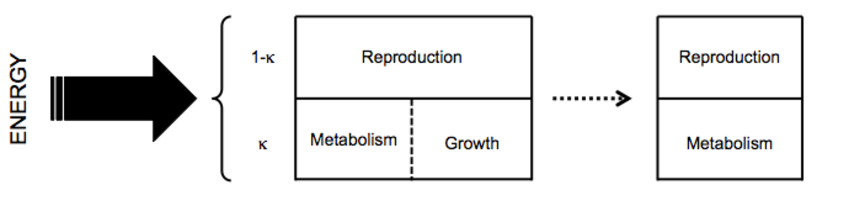
\includegraphics[width=0.95\textwidth]{1_CorpsDeThese/Resumes/Fig/AN01}
\caption[\lofimage{1_CorpsDeThese/Resumes/Fig/AN01}Règle du
$\kappa$]{Schéma de la règle du $\kappa$ et de ses implication}
\label{fig:AN1}
\end{center}
\end{figure}

Outre les interactions entre individus, le modèle se base sur les règles
d'allocation dynamique du budget énergétique \autocites{kooijman2000a}. Une fois la règle fixée, on peut en
dériver les taux vitaux individuels. 

Nous nous basons sur la règle d'allocation appelée règle du
$\kappa$ ($\kappa$-rule), schématisée par la Figure \ref{fig:AN1}. Cette règle
suppose qu'une proportion $\kappa$ de l'énergie acquise par un individu est
allouée à la maintenance (métabolisme) et à la croissance, le reste ($1-\kappa$)
étant attribué à la reproduction. Cela implique automatiquement qu'un individu à sa
taille maximum continue de se reproduire, ce qui n'est pas toujours le cas pour
d'autres règles d'allocation de l'énergie (voir Annexe \ref{An:AmNat},
Supplementary Materials \ref{subsec:SupMat4}). Lorsque l'individu ne grandit
plus, l'énergie est alors divisé en une fraction fixe pour couvrir le
métabolisme et le reste pour la reproduction. Si l'énergie acquise diminue, le
métabolisme étant fixé par la taille de l'individu, la quantité
allouée à la reproduction diminue. Si l'énergie acquise n'est pas suffisante
pour couvrir l'intégralité du métabolisme, l'individu meure.

On suppose que l'acquisition de la ressource est proportionnelle à $l^2$
et que le métabolisme est proportionnel à $l^3$, cette règle d'allocation de
l'énergie nous permet alors de définir les taux vitaux individuels tels que
décrit dans la Table \ref{tab:ANEq}. Le détail de la dérivation des équations du modèle
est disponible dans les Supplementary Materials \ref{subsubsec:SupMat21} de
l'Annexe \ref{An:AmNat}. 

\begin{table}
\centering
\caption{\label{tab:ANEq} Equations du modèle d'après la règle du $\kappa$.}
\begin{tabular}{cl}
\hline 
\hline
&\\
Equation & Description \\
\hline
	$\displaystyle{A(t,l)=1-\frac{\eta(t,l)}{\eta_{H}+\eta(t,l)}}$ & Access to the
	resource\\
	&\\
	$\displaystyle{\eta (t,l) = \int\limits_{l_b}^{l_m} C(l,\lambda)\cdot
	n(t,\lambda)\cdot \lambda^2\,\text{d}\lambda}$ & Experienced population
	density\\
	&\\
	$\displaystyle{C(l,\lambda) = \text{max}[0.01,\, 1+I\cdot(\lambda-l)]}$ &
	Competition function \\
	&\\
	$\displaystyle{g(t,l) = \gamma\cdot(l_m \cdot A(t,l)-l)}$ & Growth rate\\
	&\\
	$\displaystyle{b(t,l) = r_m \cdot A(t,l)\cdot l^2}$ & Birth rate if $l\geq
	l_j$\\
	&\\
	&\\
	$\displaystyle{\frac{\partial n(t,l)}{\partial t}+ \frac{\partial
	g(t,l)\cdot n(t,l)}{\partial l} = -\mu \cdot n(t,l) }$ & Population level
	equation\\
	&\\
	$\displaystyle{g(t,l_b)\cdot n(t,l_b) = \int\limits_{l_b}^{l_m} b(t,l)\cdot
	n(t,l) \, \text{d}l}$ & Boundary conditions \\
\hline 
\end{tabular} 
\end{table}

\subsubsection{Minimum vital d'accès aux ressources}
Nous définissons le minimum vital d'accès aux ressources comme la quantité $A^*$
telle que la croissance individuelle est nulle.

\begin{equation}
\label{eq_an4}
A^*(l) = \frac{l}{l_m}
\end{equation}
Bien que dépendante de $l$,
cette quantité est analogue au $R^*$ de Tilman dans le sens où elle définit des
conditions minimums permettant la croissance des individus. 

Les paramètres utilisés dans ce modèle sont rappelés dans la Table
\ref{tab:ANparam}. Les données expérimentales permettant de justifier ces
données sont présentées dans les Supplementary Materials \ref{subsec:SupMat1} de
l'Annexe \ref{An:AmNat}. 

\begin{table}
\caption{\label{tab:ANparam}Variables et paramètres pour \textit{Folsomia
candida}}
\begin{tabular}{cccl}
\hline
\hline 
 & & &\\
 Objects and  & Default values & Units & Description\\ 
symbols & & &\\
\hline
	$i$-state variable & & & \\ 
	$l$ &   & mm & Individual length \\ 
	Parameters & & & \\ 
	$l_{b}$ & 0.25 & mm & Length at birth \\ 
	$l_{j}$ & 0.6 & mm & Length at maturity \\ 
	$l_{m}$ & 3.0 & mm & Length at infinite\\
	& & &  resources \\ 
	$\gamma$ & 0.015 & d$^{-1}$ & Van Bertalanffy growth rate \\ 
	$\eta_{H}$ & 1000 & individuals & Half saturation constant \\ 
	$\mu$ & 0.0065 & d$^{-1}$ & Background mortality \\ 
	$r_{m}$ & 3.0 & d$^{-1}$mm$^{-2}$ & Reproduction rate \\ 
	$\kappa$ & 0.7 & -- & Fraction of energy \\
	  &   &   & intake allocated \\
	  &   &   & to reproduction \\ 
	  $I$ & 0 & -- & Level of interference\\
\hline 
\end{tabular} 
\end{table}

\subsubsection{Intégration au niveau population}

Au niveau de la population, le nombre d'individus au temps $t$ est donné par
\begin{equation}
\label{eq_an5}
\int_{l_b}^{l_m}\!n(t,l)\,\mathrm{d}l
\end{equation}
où $n(t,l)$ est le nombre d'individus de taille $l$ au temps $t$. La dynamique
de la population est alors donnée par les équations et conditions initiales
suivantes \autocites{kooijman1984a,de-roos1997a}:
\begin{align}
\label{eq_an6}
\frac{\partial n(t,l)}{\partial t}+\frac{\partial g(t,l) \cdot n(t,l)}{\partial l}=-\mu \cdot n(t,l) \\
g(t,l_b) \cdot n(t,l_b)= \int_{l_b} ^{l_m} \! b(t,l)\cdot n(t,l)\, \mathrm(d)l
\\ n(0,l)=\Psi(l)
\end{align}

\subsection{Analyse de bifurcation}

Afin d'étudier le rôle de l'interférence dans les dynamiques produites par notre
modèle, nous avons réalisé une analyse de bifurcation sur le paramètre $I$ du
modèle. Bien que cette analyse ne soit pas une analyse de continuation à
proprement parler, elle nous permet d'identifier les intervalles de paramètre
correspondant à différents types de dynamiques. 

Le principe de cette analyse est comme suit: (i) une première simulation est
exécutée avec la valeur initiale du paramètre dit de bifurcation (ici $I$)
jusqu'à ce que la population ait quitté le régime transitoire; (ii) l'état final
de la population (soit sa distribution à la fin de la simulation) est utilisé
comme état initial d'une nouvelle simulation; (iii) le paramètre d'interférence
est incrémenté; et (iv) le processus est répété jusqu'à exploration de
l'ensemble de l'intervalle voulu. Notons que cette analyse peut également être
réalisée avec des valeurs décroissantes du paramètre de bifurcation, ce qui peut
permettre d'identifier des zones de bistabilité. 

Dans un premier temps, cette analyse a été réalisée pour une valeur fixe des
paramètres excepté le paramètre de bifurcation $I$. Puis, sachant que la
mortalité a un fort effet sur la dynamique de ce type de modèle, cette analyse
a été faite pour des valeurs successives de mortalité avec le paramètre $I$
comme paramètre de bifurcation, et pour des valeurs successives d'interférence
avec le paramètre de mortalité $\mu$ comme paramètre de bifurcation. Ainsi,
l'ensemble de l'espace $(I,\mu)$ a été quadrillé pour des valeurs de $I$ de 0 à
3 et des valeurs de $\mu$ de 0.001 à 0.02

\section{Résultats}

Nous nous intéressons dans un premier temps à l'effet du niveau de compétition
par interférence pour une valeur assez faible de mortalité ($\mu = 0.0065$,
Figure \ref{fig:AN2}). 

\begin{figure}[!ht]
\begin{center}
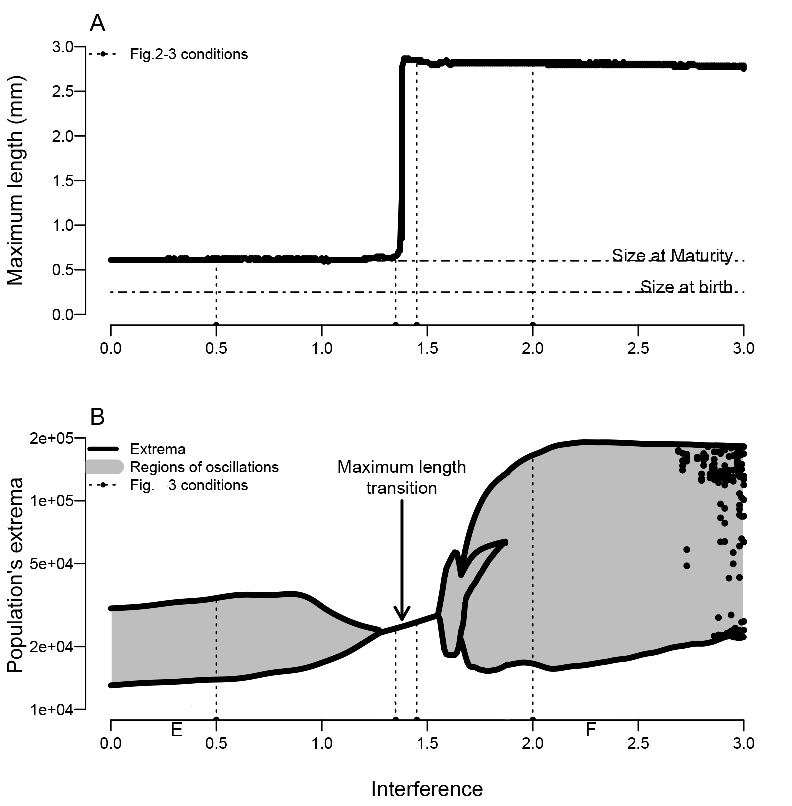
\includegraphics[width=0.95\textwidth]{1_CorpsDeThese/Resumes/Fig/AN02}
\caption[\lofimage{1_CorpsDeThese/Resumes/Fig/AN02}Bifurcation sur le
niveau d'interférence]{Taille maximum atteinte dans la population (A) et extrema
de la population (B, nombre d'individus) en fonction du niveau de compétition par interférence $I$ pour une
valeur constante de mortalité ($\mu = 0.0065$). Les lignes pointillées
représentent les valeur d'interférence des simulations présentées en Figure
\ref{fig:AN3}. Les zones grisées marquent les zones ou la population est
cyclique. La flèche marque la transition de taille maximum atteinte.}
\label{fig:AN2}
\end{center}
\end{figure}

On constate dans un premier temps qu'un niveau suffisamment élevé de compétition
par interférence ($I=1.4$) provoque une transition dans la taille maximum
atteinte par les individus (Figure \ref{fig:AN2}A). Lorsque le niveau
d'interférence est plus faible que cette valeur, la taille maximum atteint ($l=0.63mm$) reste proche de la taille à
maturité ($l_j=0.6mm$). Au delà de la valeur critique, la taille atteinte
($l=2.85mm$) se rapproche fortement de la taille maximum atteignable
($l_m=3mm$). 

De plus, la Figure \ref{fig:AN2}B montre trois régions distinctes: (i) à faible
interférence, la population est cyclique; (ii) pour un niveau intermédiaire de
compétition par interférence, la population est stable; et (iii) pour une forte
interférence, la population cycle autour d'un nouveau type de cycles de plus
grande amplitude que les précédents. 

\subsection{Des cycles dirigés par les juvéniles}

Les modèles PSP classiques prédisent qu'à faible mortalité, la différence de
capacité de compétition entre les juvéniles et les adultes conduit à des cycles
de génération dirigés par les juvéniles \autocites{de-roos1992a,de-roos1997a}.
La Figure \ref{fig:AN3}abc montre la dynamique de la population pour un faible
niveau d'interférence ($I=0.5$). On observe sur le diagramme structure-temps (a)
que la dynamique cyclique correspond à des vagues successives de recrutement de
juvéniles avec des adultes ne dépassant que très peu la taille à maturité. Cette
dynamique est caractéristique des cycles de génération dirigés par les juvéniles
\autocites{de-roos1992a,de-roos2003a}.

\afterpage{%
    \clearpage% flush all other floats
    \ifodd\value{page}
    %\else% uncomment this else to get odd/even instead of even/odd
        \expandafter\afterpage% put it on the next page if this one is odd
    \fi
    {%
    \begin{figure}[p]
        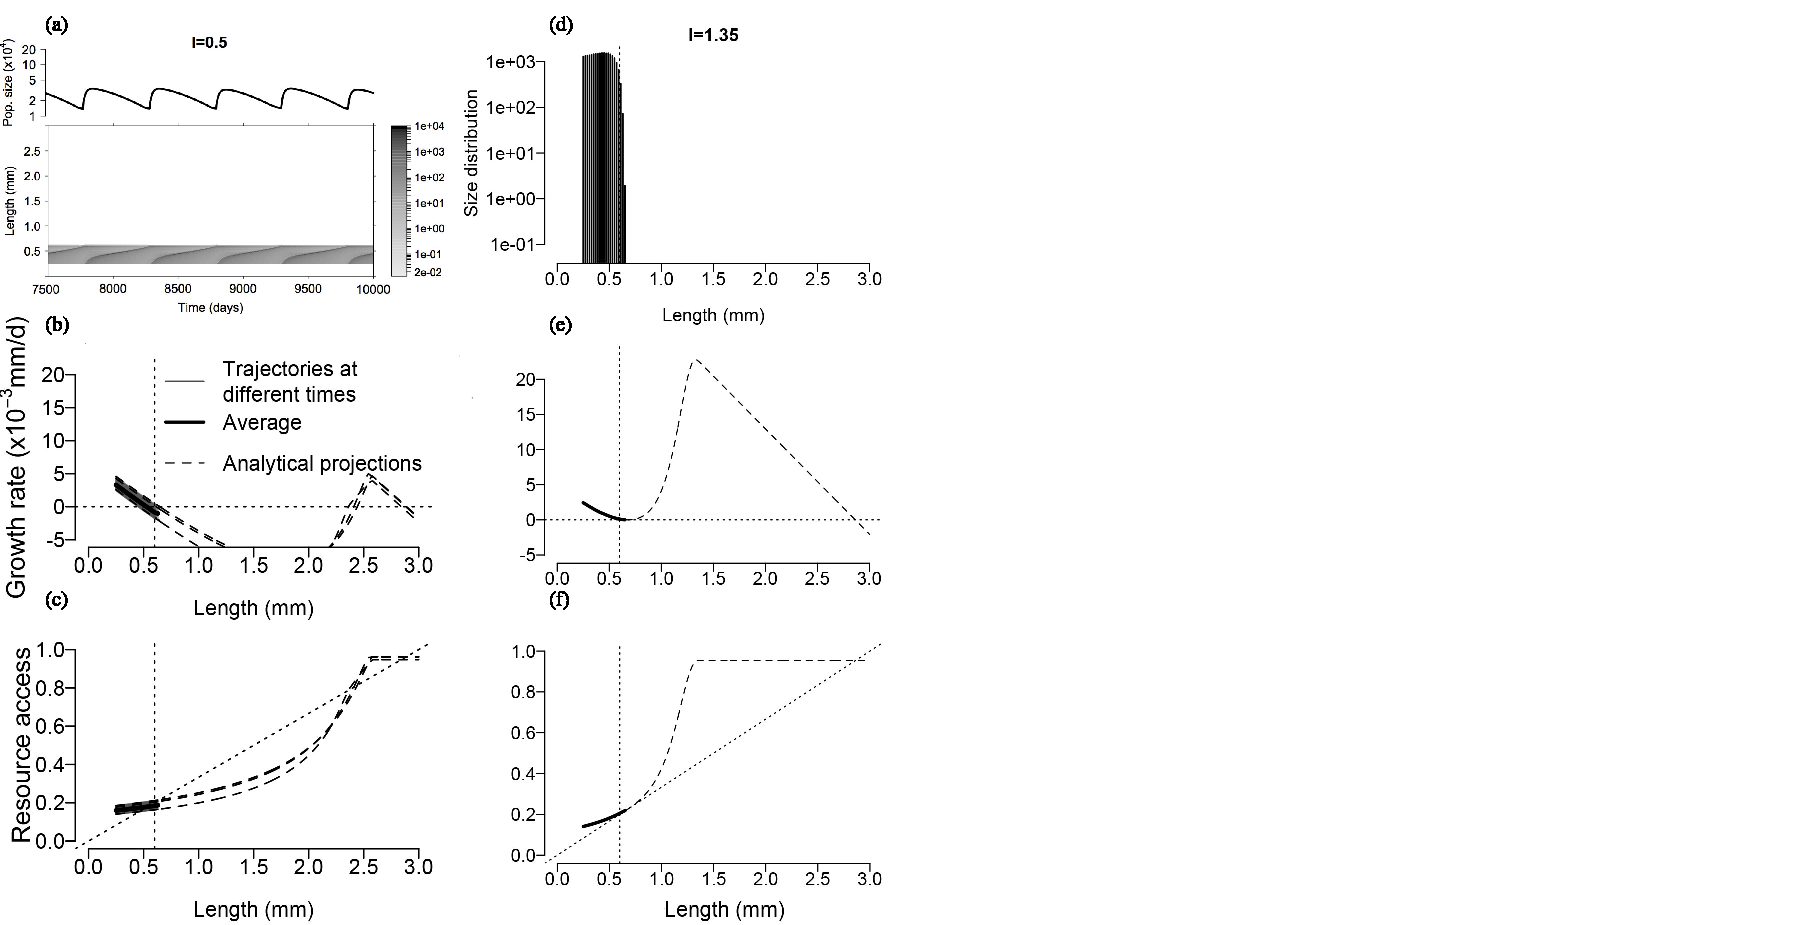
\includegraphics[width=\textwidth]{1_CorpsDeThese/Resumes/Fig/AN03}
        \caption[\lofimage{1_CorpsDeThese/Resumes/Fig/AN03}Exemples de
        dynamiques pour quatre valeurs d'interférence]{Exemples de dynamiques pour quatre valeurs d'interférence:
        0.5, 1.5, 1.45 et 2.0. La première ligne de panels (a,d,g,j) montre soit la
dynamique de la structure à l'aide d'un diagramme structure-temps (a,j), soit la
distribution de la taille si elle est stable dans le temps (d,g). La seconde
ligne (b,e,h,k) représente le taux de croissance en fonction de la longueur
corporelle\ldots}\label{fig:AN3}
    \end{figure}
    \clearpage
    \begin{figure}[p]
		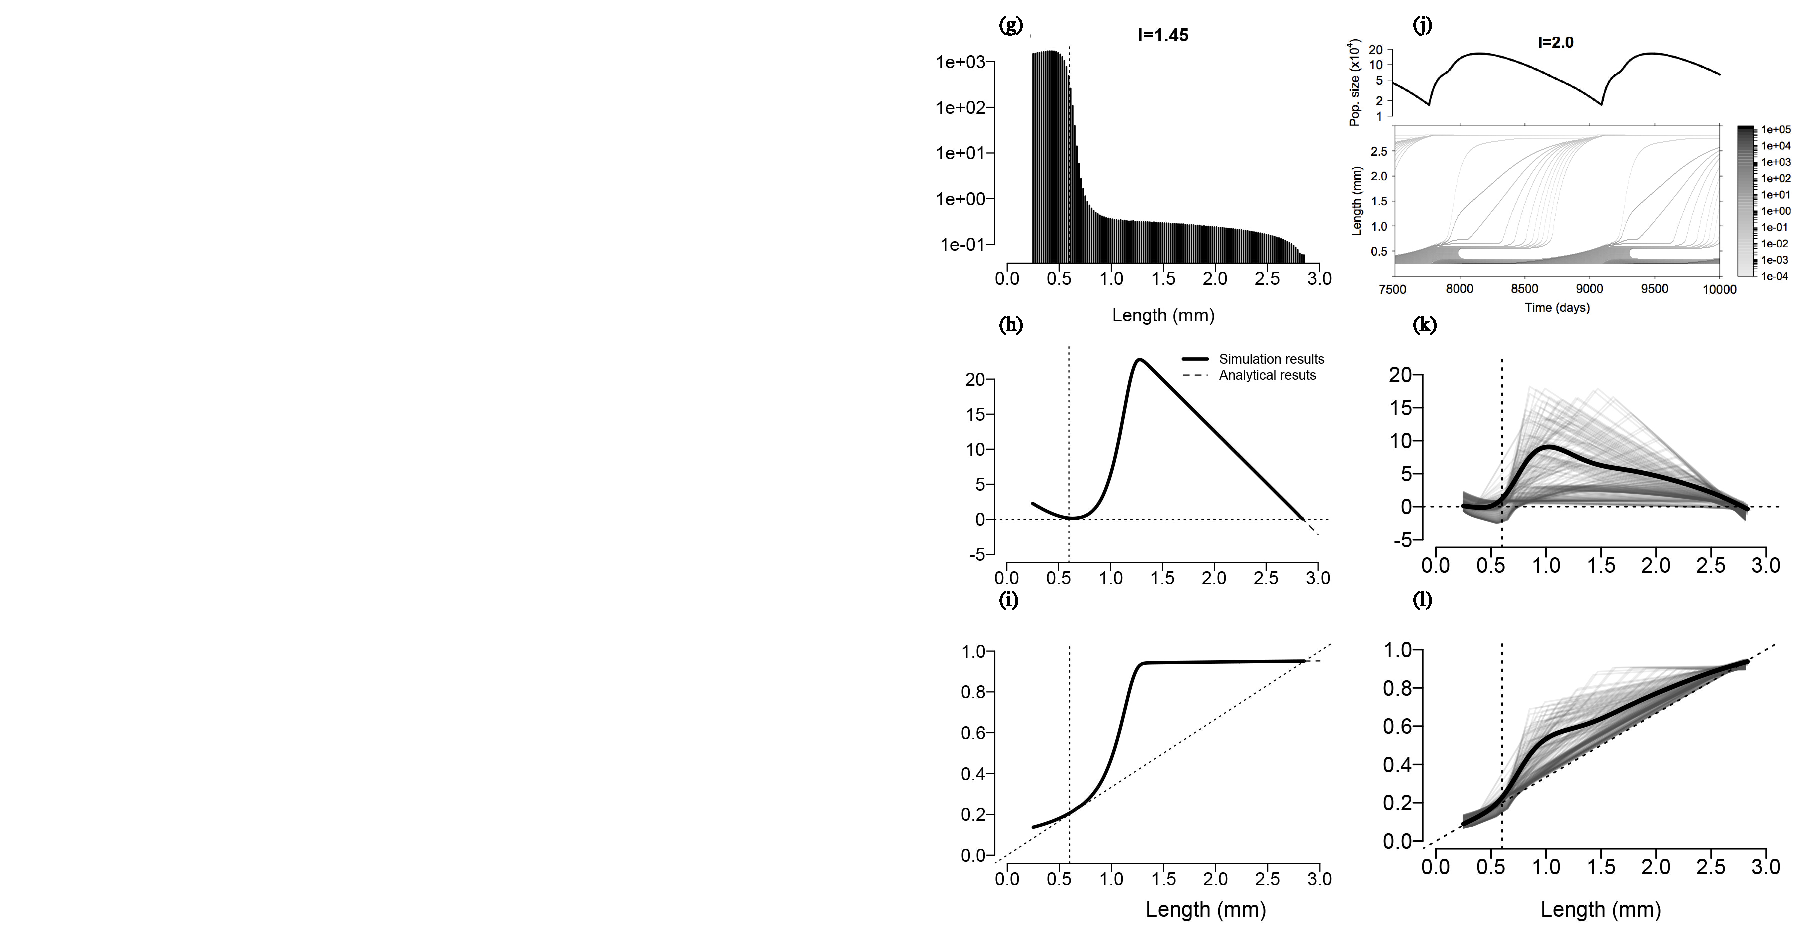
\includegraphics[width=\textwidth]{1_CorpsDeThese/Resumes/Fig/AN04}
        \caption*{\ldots Lorsque la dynamique est cyclique, plusieurs
        trajectoires sont présentées, ainsi que leur moyenne en trait épais.La ligne pointillée
horizontale est le 0, la ligne verticale marque la taille à maturité. Enfin, la
dernière ligne de panels (c,f,i,l) présente l'accès à la ressource. La ligne
verticale marque la taille à maturité, la ligne oblique marque l'accès minimum
requis $A^*$. Pour le taux de croissance et l'accès aux ressources, les lignes
tiretées représentent les projections analytique des fonctions tracées.}
    \end{figure}
    \clearpage
    }%
}

Les Figures \ref{fig:AN3}b et c montrent le taux de croissance et l'accès aux
ressources pour cette dynamique. Le taux de croissance décroît
quasi-linéairement avec la taille, de façon très similaire au modèle classique
sans interférence. L'accès aux ressources est très légèrement croissant mais
devient rapidement inférieur à $A^*$ pour tous les individus après la maturité. 

\subsection{Un équilibre stable avec des petits ou des géants}

Pour des valeurs intermédiaires de compétition par interférence, l'avantage
que les grands individus retirent de l'interférence contrebalance la compétition
par exploitation imposée par les juvéniles. Ceci vient contrer les mécanismes
de déséquilibre compétitif à l'origine des cycles de génération, et tend à
stabiliser la population (Figure \ref{fig:AN3}d-i).

Pour une valeur d'interférence sous le seuil critique de $I=1.4$, la dynamique
se stabilise autour d'une distribution étroite de la taille corporelle (Figure
\ref{fig:AN3}d). Le taux de croissance et l'accès à la ressource ont tendance à
se courber vers le haut pour les plus grands individus, mais la courbure n'est
pas suffisante pour permettre à l'accès au ressources de rester au dessus de
$A^*$, et les individus s'arrêtent de grandir rapidement après la maturation (Figure
\ref{fig:AN3}ef).

Au delà de ce seuil critique, la courbure est suffisante pour que l'accès aux
ressources soit toujours supérieur à $A^*$ et le taux de croissance soit
toujours positif (Figure \ref{fig:AN3}hi). Après un ralentissement de leur
croissance proche de la maturité (``goulet d'étranglement de la croissance''), les individus peuvent
reprendre une croissance rapide jusqu'à des tailles très élevées. La
distribution de la taille dans la population est alors très asymétrique vers les
juvéniles, mais reste continue jusqu'à des tailles proches de la taille maximum
possible $l_m$ (Figure \ref{fig:AN3}g). Les formes particulières des fonctions
de croissance et d'accès à la ressource s'expliquent d'abord par la faible
densité d'adultes au delà de $0.6mm$ et leur grande compétitivité, ils
sont donc rapidement capables de monopoliser la ressource et grandissent très
rapidement. La partie linéaire après $l=1.4mm$ est quand a elle la conséquence
de la forme naturelle de la fonction de croissance de Von Bertalanffy. 

\subsection{Des cycles induits par l'interférence}

La bifurcation sur l'interférence montre l'apparition de cycles lorsque le
niveau de compétition par interférence est suffisamment élevé ($I>1.56$ Figure
\ref{fig:AN2}). La Figure \ref{fig:AN3} (j-l) montre le détail de la dynamique
pour une valeur de compétition par interférence de $I=2.0$. On constate sur le
diagramme structure temps (j) que les cycles dans la structure de la population
sont très différents des cycles de génération induits par les juvéniles (a). La
période des cycles a été multipliée par $3$ et l'amplitude est environ $7.5$
fois supérieure. Un cycle dans la dynamique commence par un pulse de naissance
qui fait fortement augmenter la taille de la population lorsqu'une cohorte
d'individus atteint la maturité. La population est alors multi-modale avec une majorité
de juvéniles, des adultes nouvellement matures et quelques vieux individus de
très grande taille. Après le pulse de naissance, les individus qui viennent de
maturer grandissent, ce qui réduit la ressource disponible pour les individus
les plus petits qui stoppent leur croissance. Deux groupes se forment, des
juvéniles de moins de $0.35mm$ et des juvéniles et jeunes adultes entre $0.5$ et
$0.75mm$. Pendant cette période, les adultes continent de se reproduire,
augmentant la densité de juvéniles. Les individus les plus vieux commencent
ensuite à mourir, diminuant progressivement la pression de compétition sur les
jeunes adultes qui atteignent à leur tour des tailles extrêmes. La pression de
compétition est cependant maintenue sur les plus petits juvéniles qui ne peuvent
pas grandir. Le nombre d'individus reproducteur commence alors à diminuer,
réduisant progressivement la taille de la population et la pression de
compétition due à l'interférence. Quand suffisamment d'adultes sont mort, la
pression de compétition a assez diminué pour que les plus petits juvéniles
reprennent leur croissance et maturent, provoquant un nouveau cycle dans la
dynamique. 

On constate sur le panel (k) que la position du goulet d'étranglement du taux de
croissance sur l'axe des X varie entre $0.33$ et $0.55mm$ suivant le moment dans
le cycle, mais reste systématiquement inférieur à la taille à maturité
$l_j=0.6mm$, ce qui provoque l'accumulation d'individus immature dans la
population. L'accès aux ressources (l) montre le même phénomène. Les individus
n'accèdent plus suffisamment aux ressources pour poursuivre leur croissance dont
le taux devient négatif (causant une mortalité accrue). Ils arrêtent donc leur
croissance à un stade immature, ce qui fait diminuer le nombre de reproducteur
et relâche progressivement la pression de compétition par interférence. C'est
précisément la position du goulet d'étranglement sous la taille à maturité qui
déstabilise la dynamique vers ces nouveaux cycles. 

\subsection{Bifurcation dans le plan $(I,\mu)$}

Le taux de mortalité basal $\mu$ étant connu pour affecter la dynamique des
populations structurées par taille, en stabilisant la dynamique vers un point
fixe lorsqu'il augmente, nous nous somme intéressé à son effet couplé à celui du
niveau de compétition par interférence. La Figure \ref{fig:AN4} montre le type
de dynamique obtenu en fonction de la position dans le plan de paramètres
$(I,\mu)$.

\begin{figure}[!ht]
\begin{center}
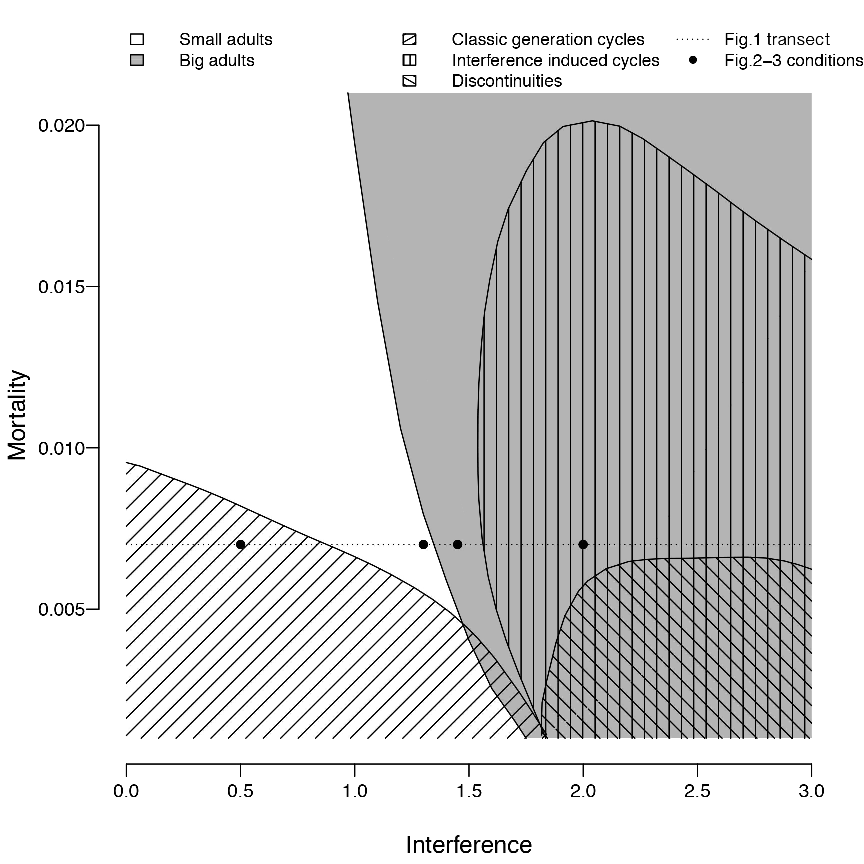
\includegraphics[width=0.95\textwidth]{1_CorpsDeThese/Resumes/Fig/AN05}
\caption[\lofimage{1_CorpsDeThese/Resumes/Fig/AN05}Diagramme de
bifurcation dans le plan $(I,\mu)$]{Diagramme de
bifurcation dans le plan $(I,\mu)$. Les régions sans hachure sont les régions
correspondant à un point fixe. Les hachures représentent le type de cycle
obtenu. La zone grise correspond à la zone de survie des individus de très
grande taille. La ligne pointillée et les points marquent respectivement la
bifurcation de la Figure \ref{fig:AN2} et les simulations de la Figure
\ref{fig:AN3}}
\label{fig:AN4}
\end{center}
\end{figure}

Dans un premier temps, on peut distinguer deux régions différentes sur ce
diagramme (régions blanches et grises) qui délimitent les zones où
la taille maximale atteinte est soit proche de la taille à maturité (en blanc),
soit proche de la taille maximum possible (en gris). Il est intéressant de noter
que la limite entre ces deux régions dépend assez peu de la mortalité basale
( $I$ entre $1.2$ et $1.6$).

On remarque également qu'en l'absence d'interférence, les cycles de génération
induits par les juvéniles sont stabilisés lorsque la mortalité basale augmente,
conformément à la théorie déjà établie \autocites{de-roos1997a}. Lorsque la
compétition par interférence est présente, cette stabilisation se produit pour
des valeurs plus basses de mortalité. De plus, l'augmentation du taux de
mortalité semble également stabiliser les cycles due à l'interférence, mais pour
des valeur très élevées ($\mu > 0.02$). 

A faible mortalité mais haut niveau d'interférence, la dynamique est irrégulière
et les résultats sont peu fiables à cause de problèmes numériques liés à
l'intégration des équations du modèle. En revanche, pour une interférence
intermédiaire et une faible mortalité, on peut observer une situation
intéressante. En effet, on constate qu'il existe une petite région où des cycles
de génération semblables à ceux dues aux juvéniles se maintiennent alors que la
taille maximum atteinte est proche de la taille maximum possible. Mais ces
cycles sont dégénérés et quelques individus parviennent de temps en temps à
s'échapper du goulet de croissance et atteindre des tailles géantes. Ces
individus sont rares et les dynamiques irrégulières. 

\section{Discussion}

Nous avons mis en évidence au cours de cette étude que la compétition par
interférence est une interaction qui, en conférant un avantage aux individus les
plus grands, vient contrecarrer les effets de la compétition taille dépendante
par exploitation. La dépendance à la taille de l'ingestion d'énergie et de son
utilisation confère un avantage aux individus les plus petits par la compétition
par exploitation \autocites{peters1986a,persson1998a,de-roos2013a} comme le
prédit la théorie du budget énergétique dynamique \autocites{kooijman2000a}.
Dans l'intervalle de niveaux de compétition par interférence que nous étudions
ici, l'équilibre compétitif entre les plus petits et les plus grands individus
bascule progressivement d'un avantage aux juvéniles, du à la compétition par
exploitation, à un avantage aux grands adultes, du à la compétition par
interférence. Entre les deux extrêmes, les compétitions par exploitation et
interférence s'équilibre et la population se stabilise. Les transitions observée
dans la Figure \ref{fig:AN2} sont très comparables à celles causées par des
modifications de la dépendance en taille de la compétition par exploitation,
telles que l'augmentation des pentes des fonctions allométriques pour le taux
d'attaque \autocites{persson1998a} ou pour le taux de consommation
\autocites{de-roos2003a}. Cependant, les mécanismes sous jacents restent très
différents. En effet, la transition vers des cycles dominés par les adultes dans
les études de \textcites{persson1998a} et \textcites{de-roos2003a} se produisent
pour des valeurs de paramètre peu réalistes. Déjà prédite par
\textcites{de-roos2003a}, notre étude propose une hypothèse alternative
conduisant à des cycles de génération dominés par les adultes.

Bien que les cycles induits par l'interférence ne soient pas strictement des
cycles dominés par les adultes (``adult driven generation cycles'') selon la
définition de \textcites{de-roos2003a}, ils partagent avec eux une
caractéristique essentielle, à savoir le fait que les oscillation reposent sur
la domination compétitive des individus les plus grands qui empêchent une
nouvelle génération de dominer la population tant qu'ils sont suffisamment
nombreux. Dans ce sens, les cycles induits par l'interférence font partie
des cycles dominés par les adultes.  

\subsection{Détecter la compétition par interférence dans des populations
naturelles} 

Le cannibalisme est un autre mécanisme qui confère un avantage aux
plus grands individus d'une population sur les plus petits en les protégeant de la
compétition par exploitation \autocites{claessen2000a,claessen2002a}, et peut
ainsi conduire à la stabilisation des cycles dominés par les juvéniles et
l'émergence d'individus de grande taille. Ces similarités font qu'il est
nécessaire d'avoir des clés permettant de discriminer différentes causes pouvant
mener aux même observations dans des populations naturelles. 

D'après nos résultats théoriques, plusieurs critères peuvent être utilisés pour
identifier le rôle de la compétition par interférence dans la dynamique d'une
population structurée. 
\begin{enumerate*}[label=(\roman*)]
\item L'observation la plus évident de l'effet de l'interférence est l'émergence
de géants dans la population. Bien que d'autres cause puissent provoquer cette
émergence telles que le cannibalisme ou une niche spécifique pour les plus
grands individus, combiné aux éléments suivant, c'est un indice en faveur
de la compétition par interférence. 
\item La présence d'un goulet d'étranglement de la croissance est un signe fort
de l'action d'une compétition par interférence assez intense.
\item Ce goulet d'étranglement provoque une distribution de la taille
fortement asymétrique en faveur des plus petits individus dans une population
stable. 
\item Dans une population cyclique, cela résulte en une distribution
multi-modale.
\item Dans les deux cas, les trajectoires de croissance individuelles
ressemblent à une double courbe de croissance. Les individus subissent un
ralentissement violent de la croissance autour de la maturité avant une
accélération brutale passé le goulet d'étranglement. 
\item L'observation des traits d'histoire de vie individuels permets donc de
distinguer les cycles causés par l'interférence des cycles dominés par les
juvéniles. Dans le dernier cas, les individus grandissent rapidement et
s'arrêtent après maturation alors que dans le premier cas la croissance s'arrête
vers la maturation pour ne reprendre que si la cohorte adulte dominante a
suffisamment diminuée. 
\item Enfin, dans le cas où les données individuelles ne sont pas accessibles,
le ratio du temps de maturation moyen par la période des cycles tel que défini
par \textcites{murdoch2002a} permet également de faire la distinction entre les
différents cycles. Comme expliqué en introduction de cette thèse
(Section \ref{modelPopStru} page \pageref{modelPopStru}), une valeur du ratio
autour de $1$ correspond à des cycles de génération. Dans notre modèle, les
cycles dominés par les juvéniles ont un ratio autour de $0.8$ alors que les cycles induits par l'interférence ont un
ratio proche de $1.5$. Ainsi, des cycles de génération avec un ratio supérieur
à 1 pourraient être une indication du rôle de l'interférence. Cela pourrait par
exemple être le cas pour les saumons dans la baie de Bristol (ratio$=1.2$) ou de
la rivière Togiak ($1.3$), la morue d'Iceland ($1.6$), le castor de Californie
(1.6), ou l'ours noir du Yukon \autocites[1.5,][]{murdoch2002a}. Ces espèces
étant territoriales, elles sont en effet susceptibles à la compétition intra-spécifique par interférence. 
\end{enumerate*}

\subsection{L'interférence dans nos populations expérimentales}

Nous avons montré dans le Chapitre \ref{chap:sp} que nos populations
expérimentales de collemboles se caractérisent systématiquement par
l'existence de plusieurs modes dans la distribution de la taille des individus.
Généralement deux, un mode assez dense de juvéniles dont la taille est proche de
la taille à la naissance, et un mode d'adultes dont la taille est très
supérieure à la taille à maturité (parfois jusqu'à plus de trois fois
supérieur). Exceptionnellement, un troisième mode peut être observé, on a alors
un premier mode de juvéniles, un mode avec des petits adultes et un mode avec
des grands adultes. Mais nous avons montré que cette situation n'était stable
que localement, et ne pouvait être atteinte qu'avec des conditions initiale de
distribution de la taille très particulières qui ne se retrouvent quasiment
jamais hors de l'initialisation des populations.

De plus, nous avons montré que les individus de grande taille jouent un rôle
prépondérant dans la dynamique de la population notamment en empêchant la
croissance des juvéniles lorsque les cohortes d'adultes sont suffisamment
denses. 

Ces observations recoupent ainsi plusieurs des critères proposés à l'issue de
notre étude théorique pour identifier le rôle de la compétition par
interférence. Cette analyse apporte des arguments supplémentaires pour confirmer
le rôle de la compétition par interférence dans la dynamique des populations de
collemboles, et confirment ainsi du même fait l'intérêt des méthodes empiriques
employées dans l'étude précédente pour extraire le rôle de
l'interférence des données.

\section{En conclusion}

Notre objectif était ici d'étudier les conséquences de la compétition taille
dépendante par interférence sur la dynamique des populations, permettant ainsi
de compléter les résultats existants sur la compétition par exploitation et le
cannibalisme comme mécanismes intra-spécifiques de régulation des populations.
Nous avons donc développé un modèle simple de dynamique de populations physiologiquement
structurées qui à notre avis rassemble les aspects essentiels de la compétition
intra-spécifique par interférence. Ce modèle n'a ainsi pas pour vocation de
prédire précisément des dynamiques de populations, bien qu'il ait été paramétré
pour les Collemboles \textit{Folsomia candida}, mais plutôt de démontrer les
conséquences dynamiques de la compétition par interférence. La comparaison avec
nos données expérimentales issues des populations de collemboles montre qu'il
est possible de détecter le rôle de la compétition par interférence dans des
populations expérimentales ou naturelles. 

Dans notre cas, nous avons pu apporter de nouveaux éléments confirmant le rôle
de la compétition par interférence dans les dynamiques des populations de
collemboles, mais il reste encore des différences entre le modèle et les séries
temporelles observées, et les mécanismes détaillés à l'oeuvre dans les
populations expérimentales ne sont encore pas éclaircis. Dans le Chapitre
suivant, nous avons mené en parallèle deux études expérimentales afin de mieux
comprendre la façon dont les individus se répartissent l'accès à la ressource,
et le rôle des individus de différentes tailles dans la dynamique de la structure
des populations.


\chapter{Confirmation du rôle de l'interférence: modification de la structure
des populations et observation de l'accès aux ressources}
\chaptermark{Confirmation du rôle de l'interférence}
\label{chap:sm}

\vspace{5cm}

\section{Introduction}

\lettrine[lines=3]{N}{otre} étude de l'effet des interactions entre individus
dans la dynamique des populations structurées nous a mené dans le Chapitre
\ref{chap:sp} à proposer la
compétition par interférence comme mécanisme responsable de la structuration
multimodale de nos populations expérimentales de collemboles \textit{Folsomia
candida} (voir aussi Annexe \ref{Ann:SP}). Au cours du Chapitre
\ref{chap:amnat} (voir aussi Annexe \ref{An:AmNat}), nous avons étudié dans un
modèle théorique les conséquences d'une compétition par interférence plus ou moins intense sur la dynamique d'une population structurée où la compétition par
exploitation entre également en jeu. Nous avons montré qu'une compétition par
interférence suffisamment intense pouvait être à l'origine d'une stabilisation
des cycles de génération dominés par les juvéniles, puis de l'apparition de
cycles de plus longue période au cours des quels des individus parviennent à
atteindre de très grandes tailles, et où la population a une structure
multimodale. Ces deux études semblent donc montrer que la compétition par
interférence est un mécanisme suffisant pour l'apparition de distributions
multimodales dans des populations structurées par la taille, et la survie
d'individus à des tailles bien supérieures à leur taille à maturité.

Suite aux résultats de notre étude théorique, nous avons voulu vérifier dans nos
populations expérimentales quel était le rôle précis des individus de
différentes tailles dans les dynamiques des structures observées, afin de
pouvoir affirmer le rôle de la compétition par interférence avec plus de certitudes.
Pour ce faire, nous avons mené deux expériences en parallèle. Dans une première
expérience nous sommes intervenus sur des populations dont la dynamique semblait
stable en perturbant la structure de la population afin d'en observer le retour
à l'équilibre et de pouvoir comparer la situation finale à celle avant la
perturbation. Cette expérience a été réalisée sur les deux clones étudiés
jusque-là, HA et TO.

Dans une seconde expérience nous nous sommes intéressés aux comportements
d'accès à la ressource dans les populations. Nous avons réalisé une série
d'observations en temps réel dans les populations afin de mieux comprendre
comment la ressource était partagée entre les individus d'une population. Ces
observations ont été réalisées dans certaines des populations de la première
expérience. Elles ont permis de comparer la distribution en taille des individus
accédant à la ressource à celle de l'ensemble de la population au moment de
l'observation. Cette comparaison a mis en évidence un accès différentiel en
fonction de la taille avec un biais quasi-systématique en faveur des individus
les plus grands dans l'accès à la ressource. 

\section{Matériel et méthodes}

\subsection{Perturbation de la structure d'une population}

Dans la première expérience, nous avons suivis des populations de collemboles
\textit{Folsomia candida} jusqu'à stabilisation de leur structure, puis nous
avons perturbé la structure afin d'observer le retour à un régime permanent. 

\subsubsection{Les populations étudiées}

Nous avons élevé et dénombré régulièrement $16$ populations de collemboles, $8$
du clone HA et $8$ du clone TO, pendant un an jusqu'à stabilisation de la
structure. Les populations ont été élevées à $21\degres$C dans les conditions
décrites dans le Chapitre \ref{chap:method}. Les populations ont été mesurées
régulièrement pour suivre leur structure en suivant également la méthode de
phénotypage haut débit présentée précédemment (voir Chapitre \ref{chap:method}
Section \ref{sec:bpsensor} et Annexe \ref{Ann:bpsensor}).

\subsubsection{Perturbation de la structure}

\paragraph{Témoins} Après 12 mois, nous considérons que la période transitoire
de la dynamique est terminée. La perturbation de la structure que nous imposons
aux populations fait intervenir un changement de boite d'élevage. Afin de
vérifier l'impact d'un changement de boite sur la dynamique de la structure
d'une population, nous conservons deux témoins pour chacun des clones pour les
quels la structure n'est pas modifiée mais la population est intégralement
transférée dans une nouvelle boite d'élevage.

\paragraph{Clone HA} Avant la perturbation de la structure les populations du
clone HA ont toutes convergé vers une distribution tri-modale de la taille
corporelle. Nous avons donc réalisé trois traitements différents, chacun sur
deux populations. Chaque traitement consiste à diviser une population en deux en
fonction de la taille des individus. La structure de la population étant séparée
en trois modes, un des modes est prélevé et isolé dans une nouvelle boite
d'élevage, tandis que les deux autres sont conservés ensemble et également
transférés dans une nouvelle boite.

Les trois modes des distributions sont désignés respectivement par les lettres J
(ou Je) pour les juvéniles, M (ou Mo) pour le premier mode d'adultes de
taille moyenne, et G (ou Gd) pour le mode d'adultes de grande taille. Les
différents traitements consistent donc à \begin{enumerate*}[label=(\roman*), before=\unskip{ : }, itemjoin={{ ; }},
itemjoin*={{ ; et }}]
\item isoler la cohorte Je et conserver les cohortes M et G dans une population
MG
\item isoler la cohorte Mo et conserver les cohortes J et G dans une population
JG
\item isoler la cohorte Gd et conserver les cohortes J et M dans une population
JM (Figure \ref{fig:SM0}).
\end{enumerate*} 
Après la séparation des cohortes, les populations nouvellement fondées sont
replacées dans les conditions d'élevage habituelles et dénombrées et mesurées
régulièrement pendant $15$ mois pour observer la période de transition et le
retour à une structure stable. 

\begin{figure}[!ht]
\begin{center}
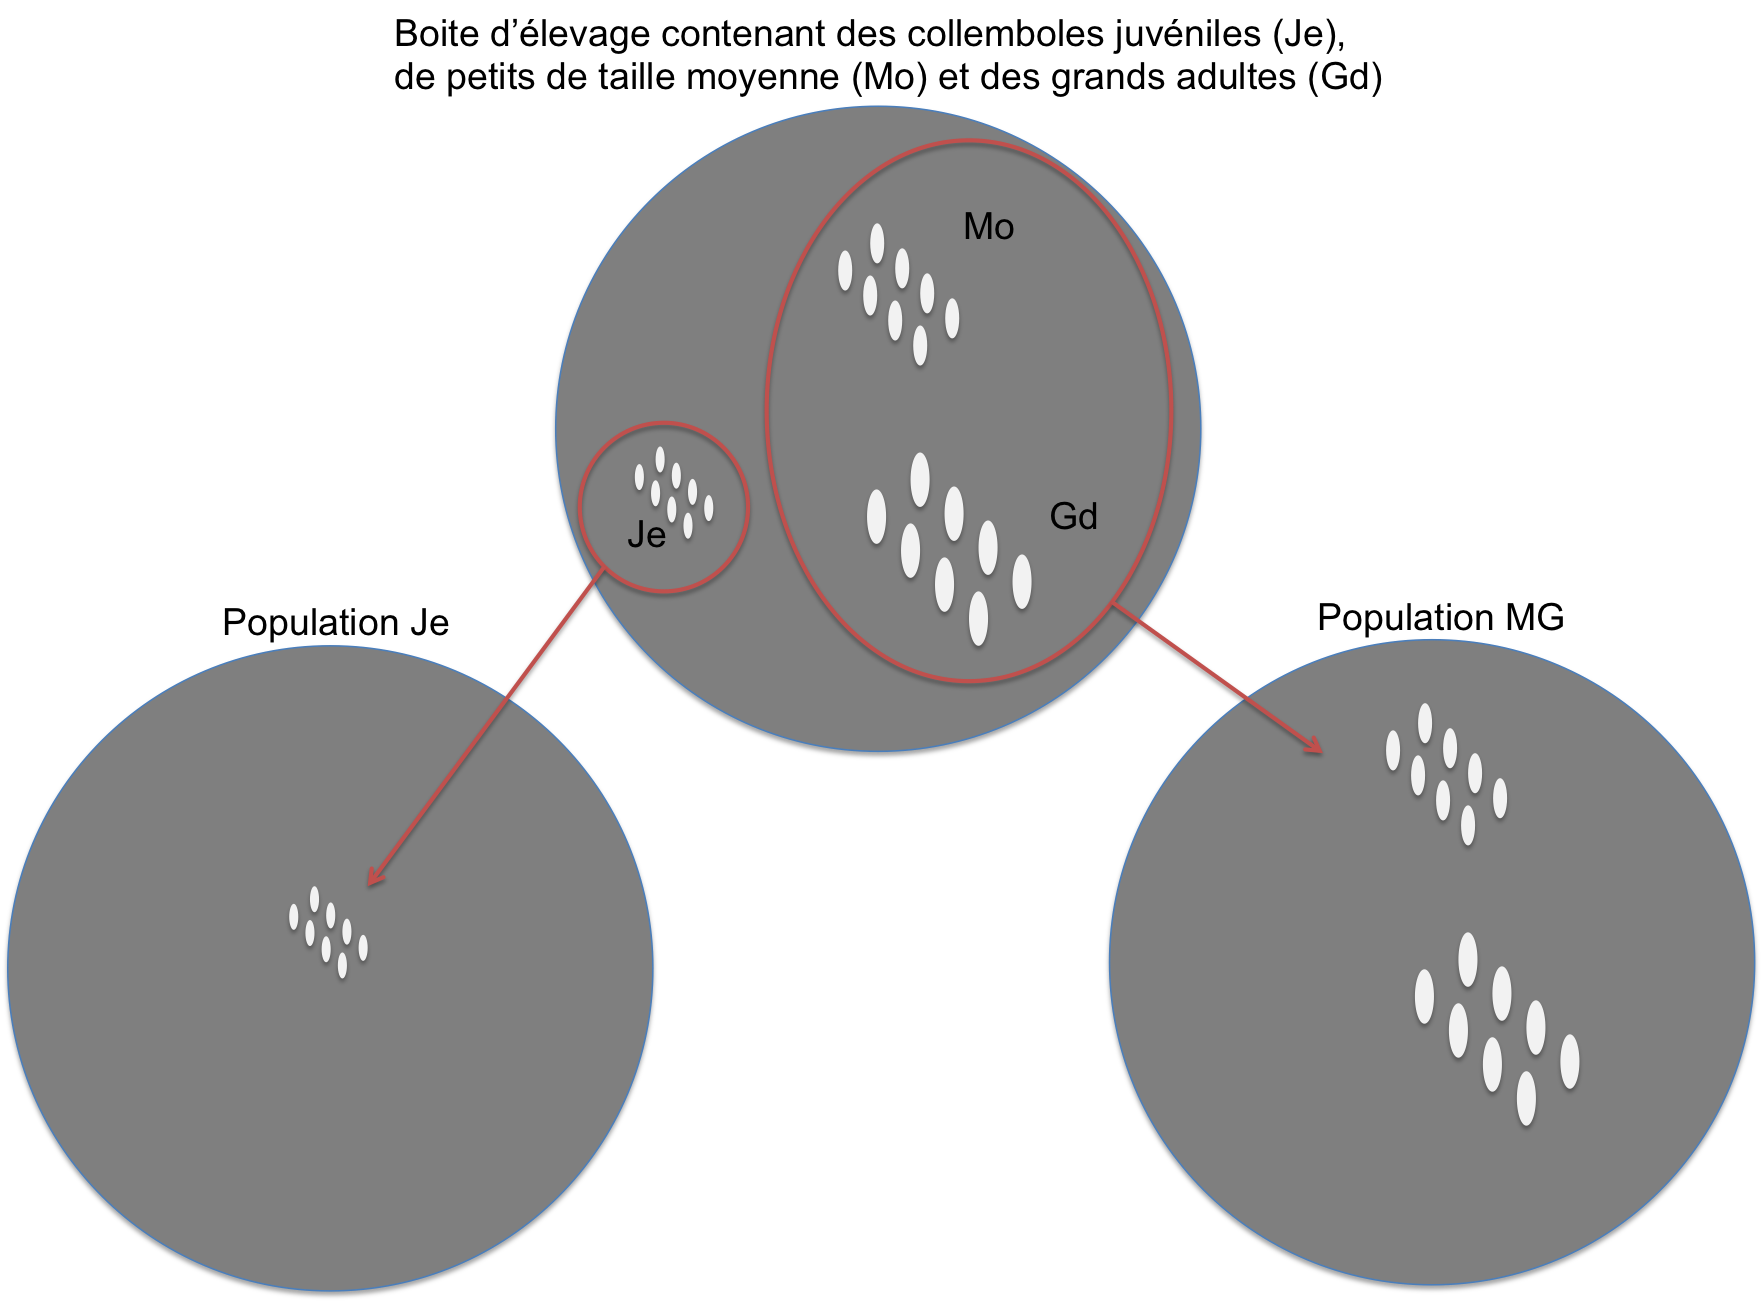
\includegraphics[width=1\textwidth]{1_CorpsDeThese/Resumes/Fig/SM00}
\caption[\lofimage{1_CorpsDeThese/Resumes/Fig/SM01}Exemple de
séparation d'une population]{Exemple de
séparation d'une population pour un traitement Je - MG.}
\label{fig:SM0}
\end{center}
\end{figure}


\paragraph{Clone TO} Contrairement au clone HA, les populations du clone TO ont
convergé au cours de la première phase de l'expérience vers des structures
bimodales. L'analyse des populations HA a montré que les adultes se répartissent
en moyenne en $\frac{2}{3}$ de petits adultes et $\frac{1}{3}$ de grands
adultes. Afin de conserver des manipulations comparables entre les clones HA et
TO, et mettre les nouvelles populations dans des conditions similaires entre les
deux clones, nous avons décidé de séparer la cohorte d'adultes en un groupe
contenant deux tiers des individus (M) et un groupe contenant le tiers restant
(G) afin de suivre les mêmes traitements que pour le clone HA. Les individus
sont choisis au hasard pour être attribué à M ou G.
Ainsi, les traitements sont \begin{enumerate*}[label=(\roman*), before=\unskip{ : }, itemjoin={{ ; }},
itemjoin*={{ ; et }}]
\item isoler la cohorte Je et conserver ensemble tous les adultes (MG)
\item isoler deux tiers des adultes (Mo) et conserver les cohortes J et le reste
des adultes G (JG)
\item isoler un tiers des adultes (Gd) et conserver les cohortes J et deux tiers
des adultes M (JM).
\end{enumerate*} 
Les nouvelles populations sont suivies pendant $15$ mois pour observer la phase
transitoire et observer le nouvel équilibre. 

\begin{figure}[!ht]
\begin{center}
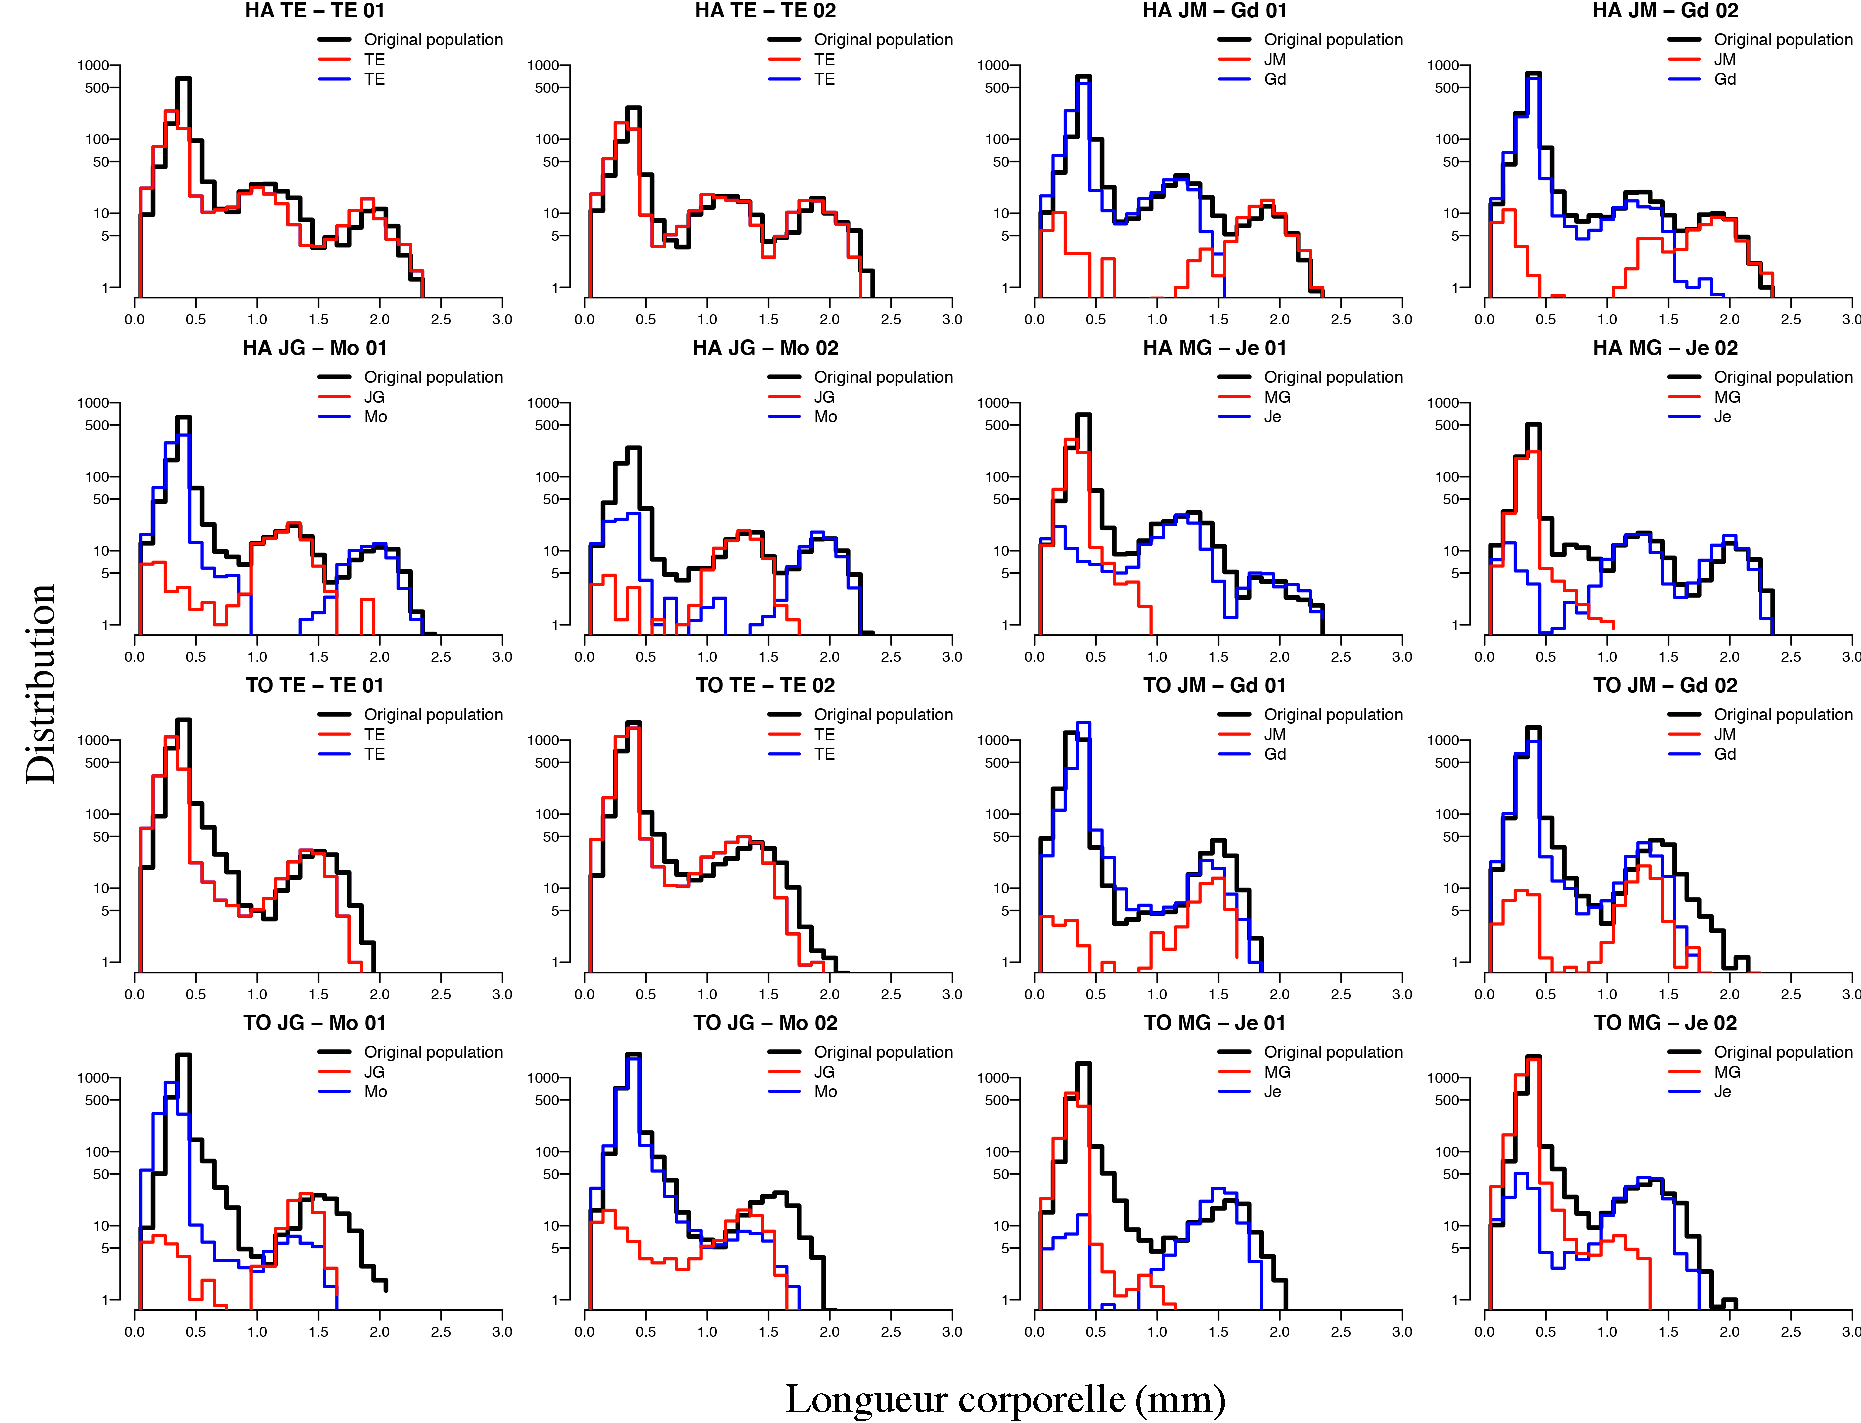
\includegraphics[width=1\textwidth]{1_CorpsDeThese/Resumes/Fig/SM01}
\caption[\lofimage{1_CorpsDeThese/Resumes/Fig/SM01}Séparation des
populations]{Résultat de la séparation des populations en deux en fonction de
la taille des individus. La ligne noire est la population d'origine, les lignes
bleues et rouges sont les populations séparées. Je, Mo et Gd se réfèrent
respectivement aux cohortes J, M et G.}
\label{fig:SM1}
\end{center}
\end{figure}

Afin de vérifier le résultat des séparations des populations en deux, nous avons
tracé pour chaque population, sur un même graphique, la distribution de la
taille dans la population d'origine et dans chacune des deux nouvelles
populations. L'ensemble des graphiques obtenus est présenté sur la Figure
\ref{fig:SM1}

\subsubsection{Analyse des dynamiques}

Les dynamiques des structures avant et après perturbation sont analysées grâce
aux diagrammes structure-temps (Chapitre \ref{chap:method} Section \ref{sec:stdiag} et
Annexe \ref{Chap:STDiag}).
Les structures après stabilisation sont alors comparées aux structures avant perturbation et
aux autres traitements. 

\subsection{Accès à la ressource}

Dans la seconde expérience de cette étude, nous réalisons une série d'analyses
\textit{in-situ} des comportements d'accès aux ressources.

\subsubsection{Observations comportementales}

La ressource est composée d'une pastille de quelques millimètres de diamètre de
levure de bière dissoute dans 15$\mu$L d'agar-agar. Afin d'observer les
comportements individuels d'accès à cette ressource, nous avons placé les boites
observées dans une étuve à 21$\degres$C, sous un microscope USB permettant une
observation en temps réel de la surface de la boite. Nous avons alors pris une
série de 10 photographies de la zone de la boite contenant la pastille de
ressource. Les clichés ont été pris avec 15 minutes d'intervalle afin de pouvoir
considérer une indépendance temporelle entre les photos. Au cours de ces
observations, la pastille est principalement consommée par le dessus, la surface
de ressource accessible pendant la période d'observation varie donc peu.

\begin{figure}[!ht]
\begin{center}
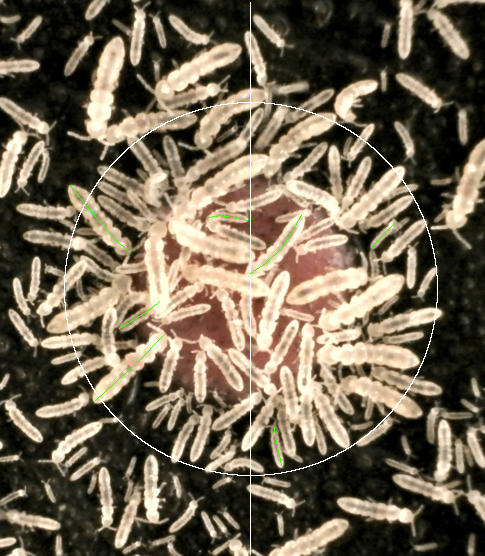
\includegraphics[height=0.25\textheight]{1_CorpsDeThese/Resumes/Fig/SM01b}
\caption[\lofimage{1_CorpsDeThese/Resumes/Fig/SM01}Exemple de comptage
sur une pastille]{Exemple de comptage
sur une pastille, les individus inclus dans le cercle sont comptés,
partiellement ou totalement à gauche, totalement uniquement à droite. Les
lignes vertes montrent le comptage et la mesure de quelques individus.}
\label{fig:SM1b}
\end{center}
\end{figure}

Les séries de photographies récoltées permettent de mesurer la taille des
individus accédant à la ressource à 10 moments que l'on considère indépendants.
L'ensemble des individus accédant à la ressource est mesuré à la main à l'aide
du logiciel d'analyse d'image ImageJ (Figure \ref{fig:SM1b}). Sur chacune des
photos analysées, la pastille est coupée verticalement en deux. Sur une des moitiés, l'ensemble des
individus en contact avec la pastille sont comptés, qu'ils soient partiellement
ou intégralement sur la pastille. Sur la seconde moitié, seuls les individus
intégralement sur la pastille sont mesurés. Ainsi on obtient dix distributions
de la taille des individus accédant à la ressource, dont on compare la moyenne à
la distribution de la taille dans la population totale.

\subsubsection{Mesure du biais d'accès aux ressources}

La distribution de la taille des individus accédant à la ressource comparée à
celle dans la population totale nous permet de mesurer un biais de taille
corporelle dans l'accès aux ressources.

\begin{figure}[!ht]
\begin{center}
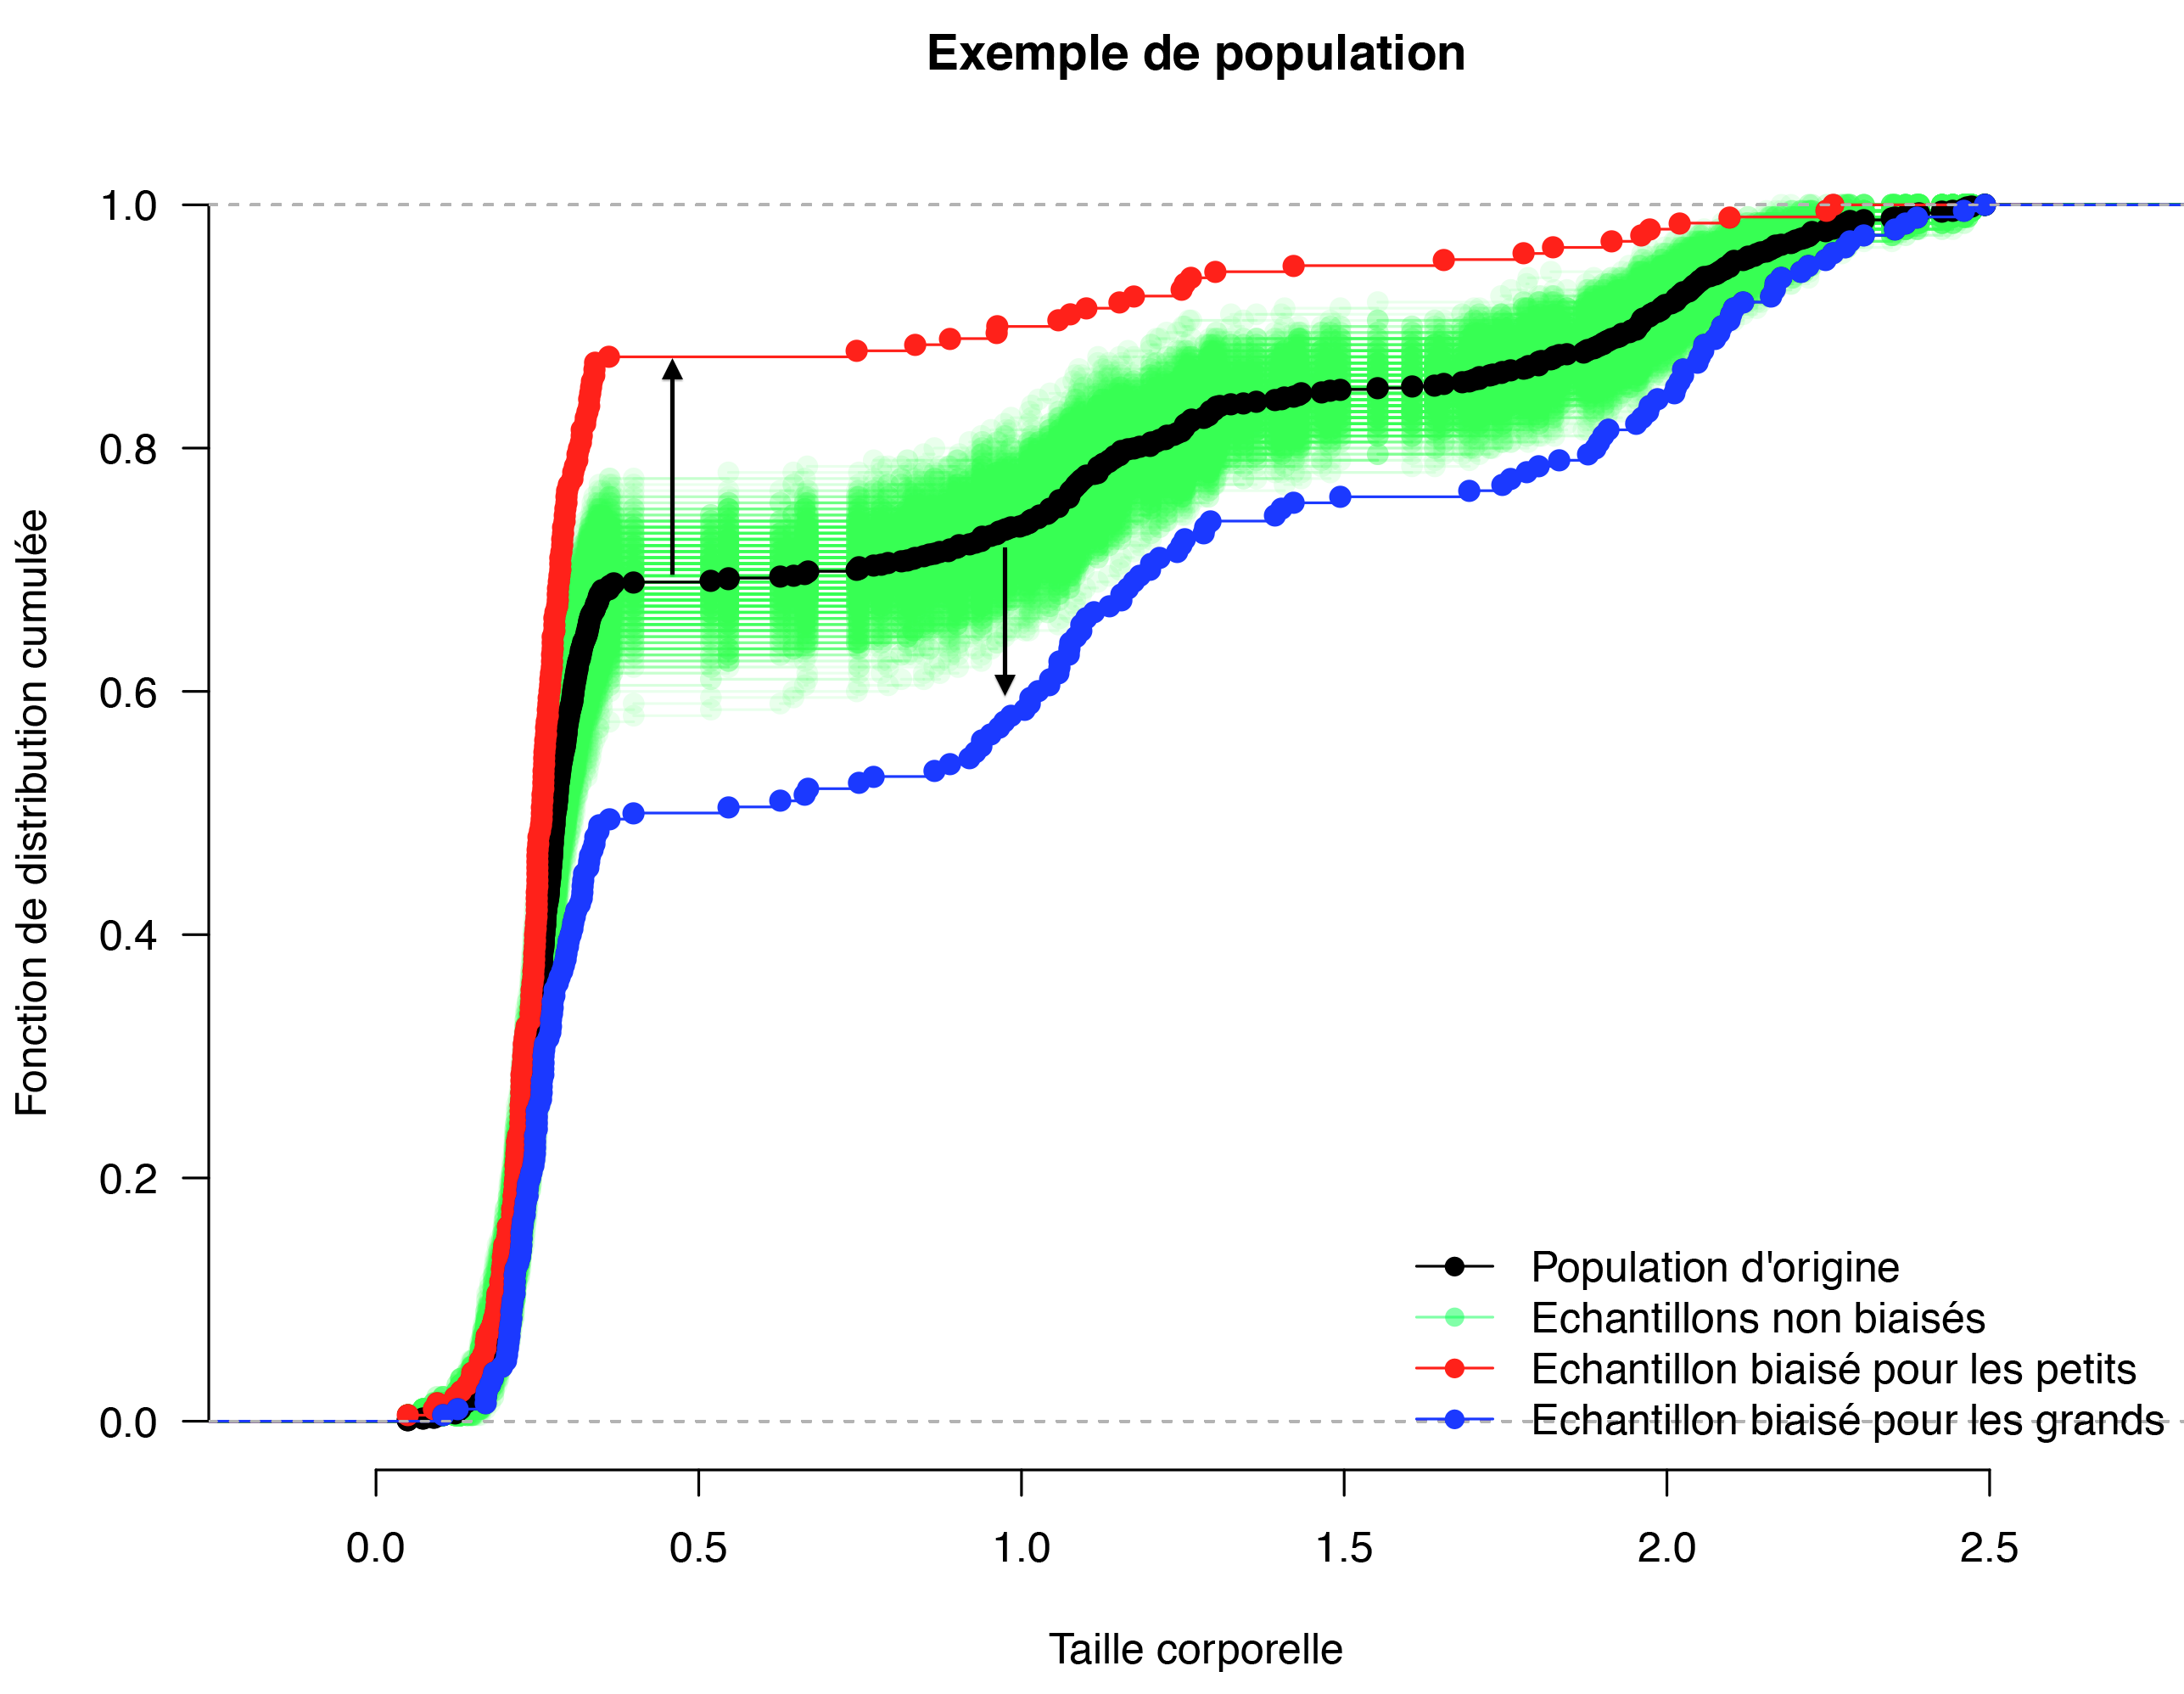
\includegraphics[width=0.66\textwidth]{1_CorpsDeThese/Resumes/Fig/SM02}
\caption[\lofimage{1_CorpsDeThese/Resumes/Fig/SM02}Comparaison des
distributions cumulées]{Exemple de comparaison des distributions cumulées entre
une population totale hypothétique (890 individus) et différents échantillons de
cette population (200 individus).
}
\label{fig:SM2}
\end{center}
\end{figure}

Les différences de distribution en taille des individus qui accèdent à la
ressource sont mesurées et comparées à la population originale en comparant les
fonctions de distribution cumulées de la taille (Figure \ref{fig:SM2}). Nous
utilisons les tests de Kolmogorov-Smirnov (KS) à deux échantillons afin de
tester la significativité de la différence et sa direction. Si la distribution cumulée
de la taille des individus accédant à la pastille est au-dessus de celle de la
population totale, cela signifie qu'il y a en proportion d'avantage de petits
individus accédant à la pastille de ressource que dans la population totale
(Figure \ref{fig:SM2}, échantillon rouge). A l'inverse, si la fonction de
distribution cumulée de la taille des individus accédant à la pastille est en
dessous de celle dans la population totale, cela signifie qu'en proportion, plus
d'individus de grande taille se trouvent sur la ressource que dans la population
totale (Figure \ref{fig:SM2}, échantillon bleu).

Les individus qui accèdent à la ressource représentent un sous-échantillon de la
population totale. Même si le test KS est significatif, nous avons vérifié que
cet échantillon est significativement différent d'un échantillon de même taille
tiré aléatoirement dans la population. Pour chaque population observée, nous
avons tiré aléatoirement $1000$ échantillons de même taille que celui des
individus accédant aux ressources afin de créer un intervalle de confiance des
échantillons aléatoires de la population totale (Figure \ref{fig:SM2},
échantillons verts). Si la distribution des individus accédant aux ressources
est en dehors de cet intervalle, cela confirme que le biais mesuré par le test KS
n'est pas dû au hasard.

% Afin d'avoir une mesure de ce biais et de sa direction, nous comparons la
% distance entre la distribution cumulée de la taille dans la population d'origine
% et la distribution moyenne de la taille des individus accédant à la ressource.
% La distance est calculée comme étant l'aire entre les deux courbes. La distance
% est soit absolue, il s'agit alors simplement de la mesure de l'aire entre les
% deux courbes, soit relative, il s'agit alors d'une aire positive si la
% distribution de l'échantillon est au dessus de celle de la distribution
% d'origine, négative si elle est en dessous. On peut alors tracer sur un graphe
% la distance relative en fonction de la distance absolue (\ref{fig:SM2}b). La
% position du point donne une indication de la direction et de l'intensité du
% biais.



\section{Résultats}

\subsection{Manipulation de la structure}

Les diagrammes structure-temps des populations témoins sont montrés figure
\ref{fig:SM3} et les populations manipulées sont présentées sur la Figure
\ref{fig:SM4}.

\begin{figure}[!ht]
\begin{center}
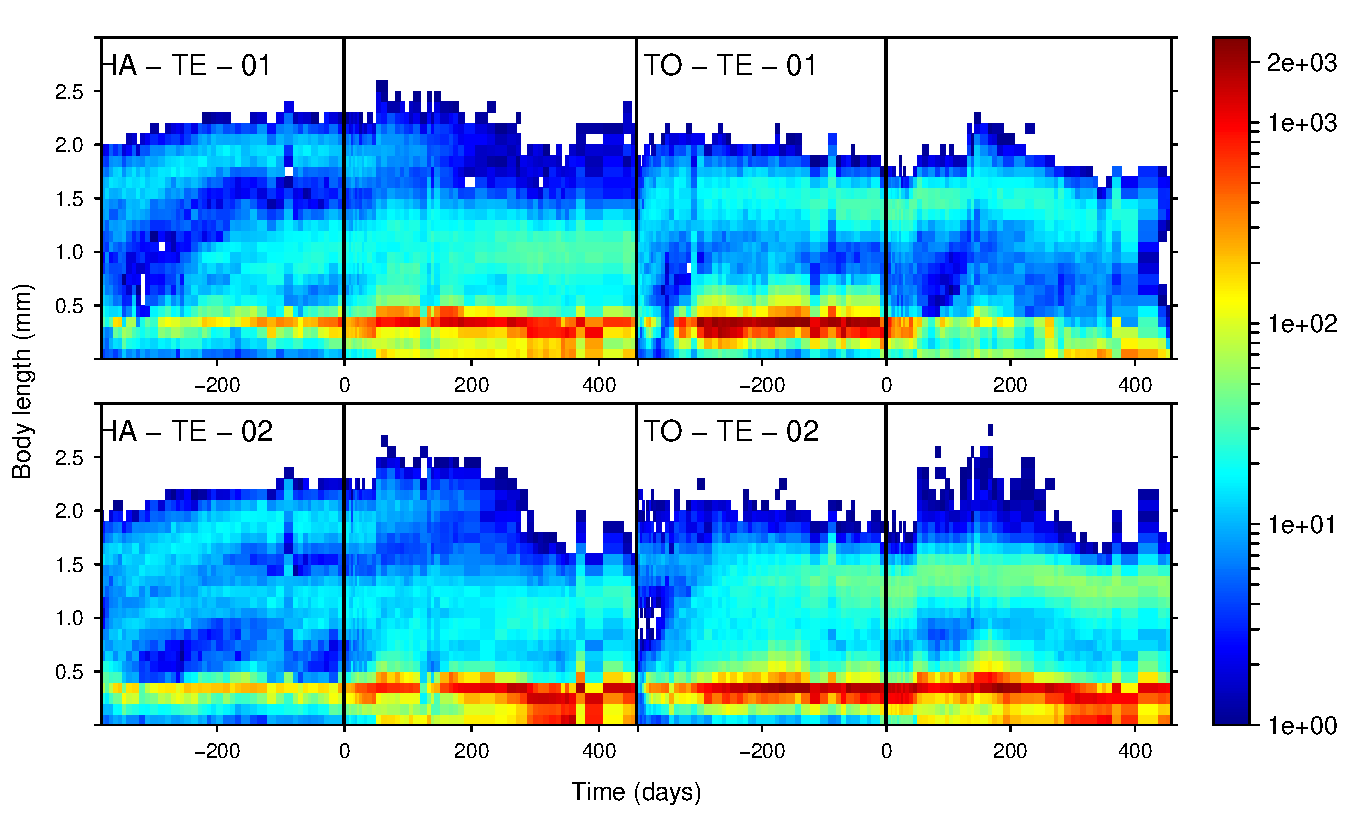
\includegraphics[width=1\textwidth]{1_CorpsDeThese/Resumes/Fig/SM04}
\caption[\lofimage{1_CorpsDeThese/Resumes/Fig/SM04}Population
témoins des clones HA et TO]{Population
témoins des clones HA et TO. La ligne vertical à la date 0 marque le moment où
les populations ont été manipulées.}
\label{fig:SM3}
\end{center}
\end{figure}

Dans les populations témoins, on constate que le changement de boite d'élevage
n'a pas eu d'effet immédiat sur les dynamiques des structures de populations. En
effet, on ne remarque pas de changement abrupt dans la structure de la
population au moment du transfert. Au contraire, les dynamiques observées
peuvent être comparées aux dynamiques présentées dans les Chapitre \ref{chap:sp}
(voir aussi Annexe \ref{Ann:SP}). Chez le clone HA, les deux populations témoins
sont trimodales au moment du transfert de boite d'élevage. Il semble que dans
les deux boites le mode des adultes les plus grands soit déjà décroissant au
moment du transfert et il s'éteint quelque temps après. Le temps de survie de ce
mode dans chacune des populations est de l'ordre de 500 jours, ce qui correspond
aux durées observées dans les populations non manipulées du Chapitre
\ref{chap:sp} (voir aussi Annexe \ref{Ann:SP}). Les deux populations TO montrent
également des dynamiques similaires aux populations non manipulées. On ne
constate pas de modification majeure dans la dynamique suite au transfert des
populations dans une nouvelle boite d'élevage.

\subsubsection{Traitements 1: Je - MG}

Dans ce traitement, la classe des juvéniles (Je) est isolée dans une boite alors
que les petits et grands adultes sont conservés ensemble et placés également
dans une nouvelle boite. Que ce soit pour le clone HA ou TO, on constate dans
les populations de juvéniles isolés le démarrage de la croissance d'une grande
partie des juvéniles dès le jour 0 (jour du transfert). Les ressources étant
apportées dans la même quantité qu'avant la manipulation, on observe l'effet du
relâchement de la compétition qui donne la possibilité aux juvéniles de grandir.
La cohorte qui démarre une croissance est très dense et conduit la structure de
la population vers une structure de type 1 (Chapitre \ref{chap:sp} et Annexe
\ref{Ann:SP}) avec des petits adultes en grande quantité et un grand nombre de
juvéniles. Dans ce traitement, les dynamiques des clones HA et TO sont très
semblables. En effet, le nombre de juvéniles qui maturent d'un coup est
suffisamment important pour empêcher HA d'exprimer sa capacité à produire des
adultes de grande taille.

\afterpage{%
    \clearpage% flush all other floats
    \ifodd\value{page}
    %\else% uncomment this else to get odd/even instead of even/odd
        \expandafter\afterpage% put it on the next page if this one is odd
    \fi
    {%
    \begin{figure}[p]
        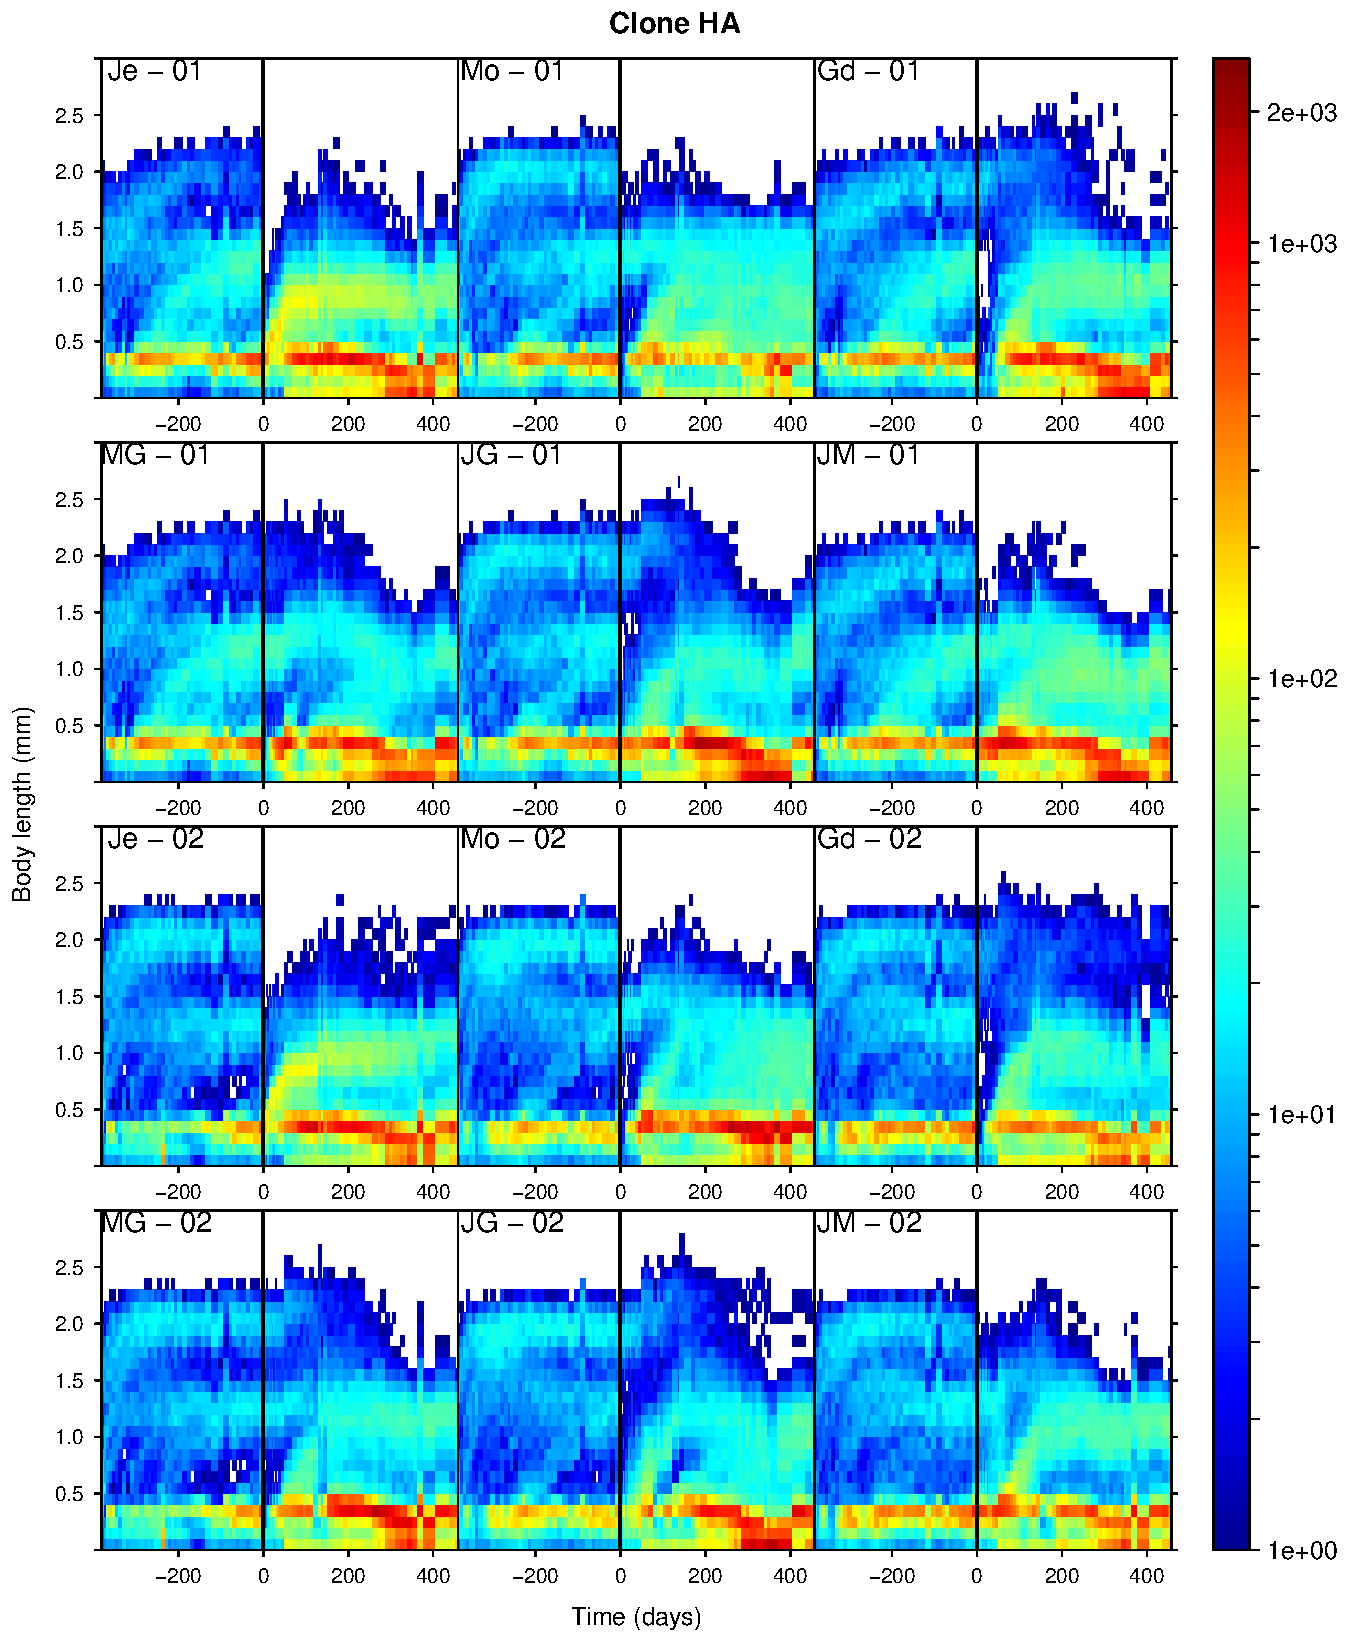
\includegraphics[width=\textwidth]{1_CorpsDeThese/Resumes/Fig/SM03a}
        \caption[\lofimage{1_CorpsDeThese/Resumes/Fig/SM03a}Diagrammes
        structure-temps des populations manipulées]{Diagrammes
        structure-temps des populations manipulées. La ligne vertical à la date 0 marque le moment où les populations ont été
        manipulées. Clone HA\ldots}\label{fig:SM4}
    \end{figure}
    \clearpage
    \begin{figure}[p]
		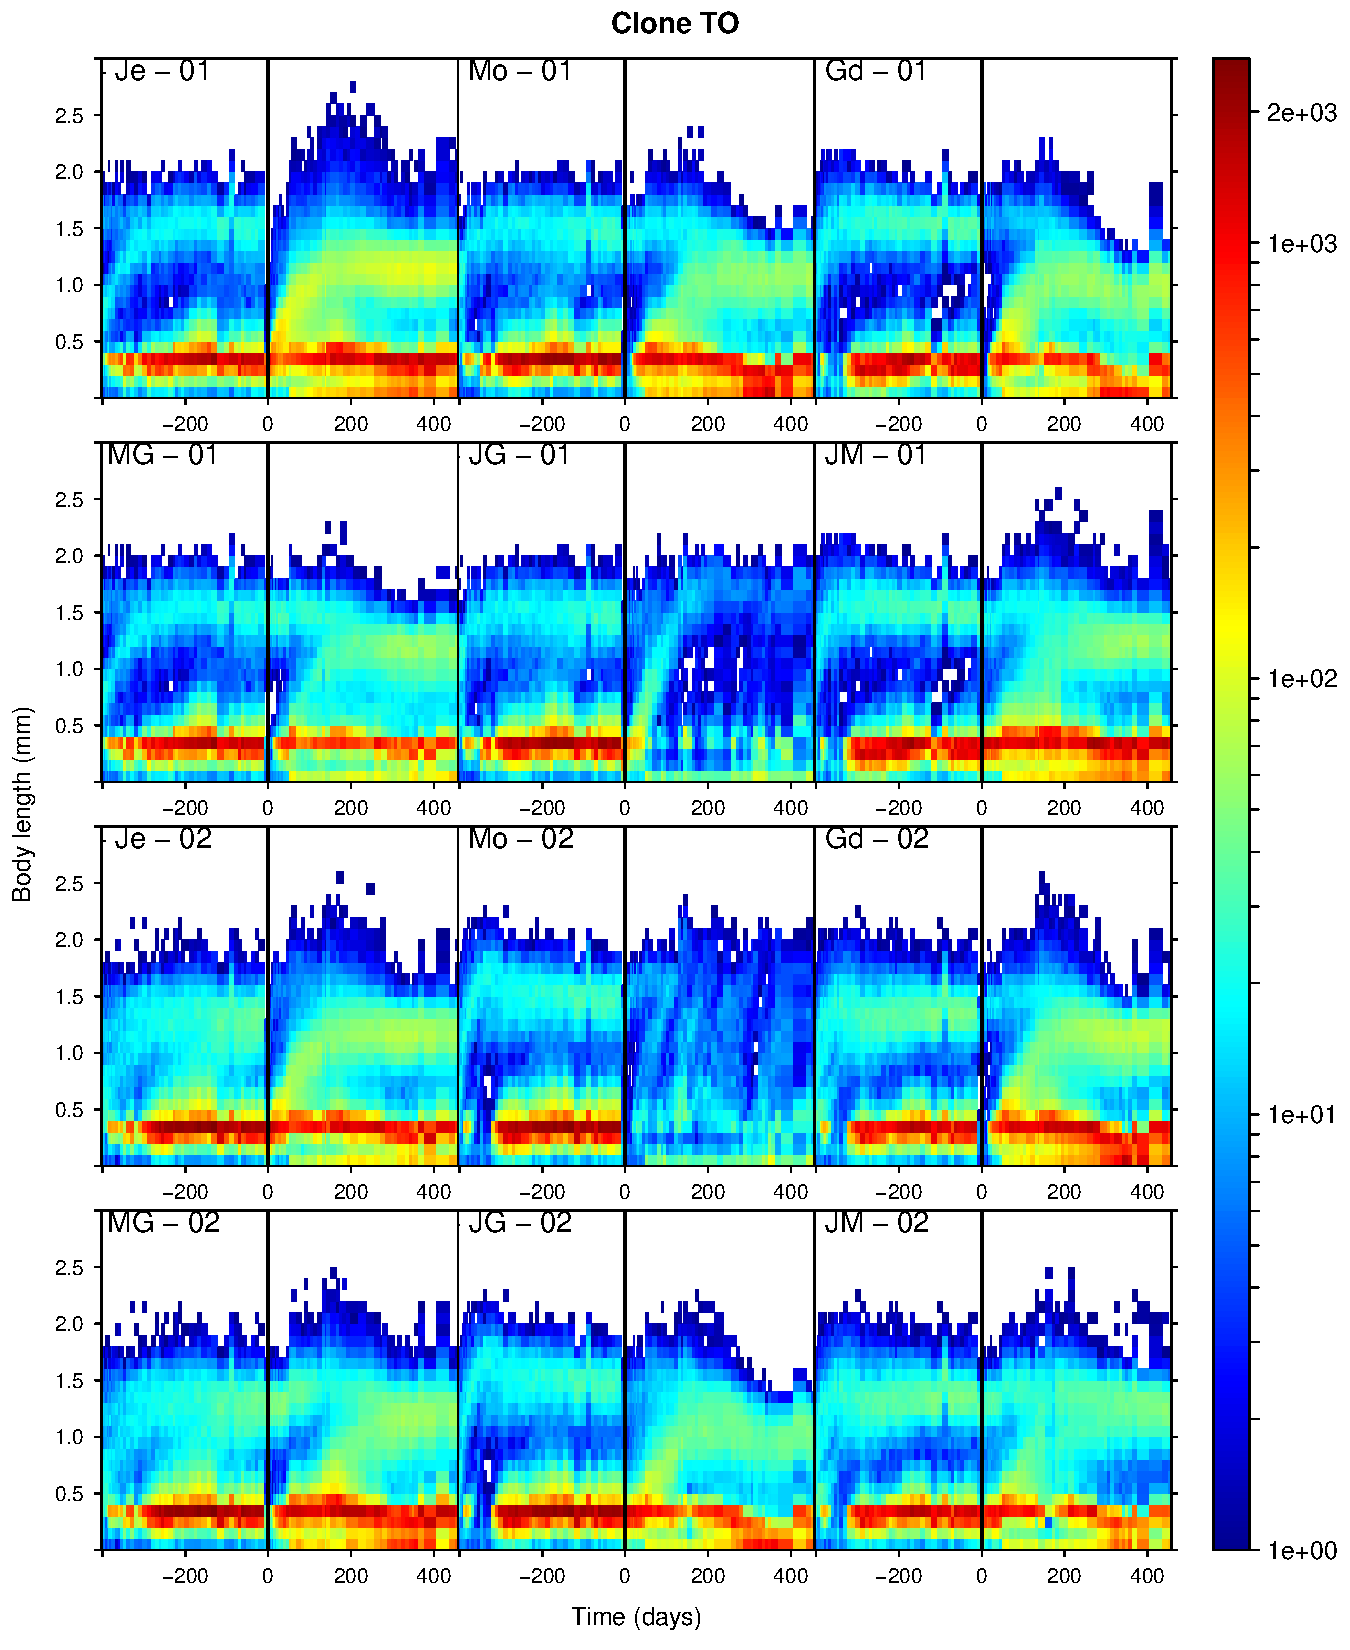
\includegraphics[width=\textwidth]{1_CorpsDeThese/Resumes/Fig/SM03b}
        \caption*{\ldots et Clone TO.}
    \end{figure}
    \clearpage
    }%
}



Dans les populations des adultes (MG), on constate chez HA que dès la
séparation les adultes reprennent également de la croissance. Ceci coïncide
également avec une disparition de la cohorte des adultes les plus grands. Cette
reprise de croissance semble montrer que malgré leurs faibles capacités
d'interférence, les juvéniles, de part leur grand nombre, exerce quand même une
pression de compétition par exploitation sur les adultes, limitant leur
possibilité de croissance. D'un point de vue de la dynamique de la structure,
dès la séparation, les adultes ont pondu et de nouvelles éclosions surviennent
après quelques semaines. On se retrouve alors de nouveau dans une situation
proche des structures de type 1 (Chapitre \ref{chap:sp} et Annexe \ref{Ann:SP}).
Ainsi, malgré le relâchement de la compétition par exploitation, les adultes les plus grands finissent par s'éteindre comme
dans les populations témoins, et ne sont pas remplacés. 

Chez le clone TO, la situation est similaire, avec un léger ajustement de la
taille immédiatement après la séparation de la population. Mais cet ajustement
s'accompagne de ponte très importantes et de nombreuses éclosions suivies de
la croissance d'une cohorte qui ramènent de nouveau les populations vers une
structure composée de petits adultes et d'un grand nombre de juvéniles.
Ainsi, le retrait des juvéniles n'a que peu d'effet car les adultes renouvellent très rapidement le
pool de juvéniles grâce à leur grande capacité de ponte. En quelques semaines,
les populations ont absorbé la perturbation et la dynamique semble peu affectée.
Il semble que ce soient les adultes de la population qui soient
responsable de la résilience de sa structure en taille: le retrait des juvéniles
modifie peu la dynamique de la structure, alors que le retrait de l'ensemble des
adultes a un effet important sur cette dynamique et peut faire basculer entre
différents types de structure. 

\subsubsection{Traitements 2: Mo - JG}

Dans ce traitement, les adultes de taille intermédiaire (Mo) sont isolés et les
juvéniles et les grands adultes (JG) sont conservés ensembles.

Chez les deux clones, l'isolation des adultes moyens (clone HA) ou de deux tiers
des adultes (clone TO) provoque une légère reprise de croissance accompagnée de
larges pontes et de la croissance d'une cohorte, qui ramène les populations dans
une structure semblable au traitement MG. Encore une fois, le retrait d'une
partie de la population relâche la compétition, ce qui explique la reprise de croissance,
mais celle-ci n'est pas suffisante comparée à la croissance des juvéniles pour
que les adultes HA atteignent les tailles du groupe de géant, ce qui ne permet
pas aux populations HA de retrouver une structure trimodale. Chez TO, la
deuxième population (TO Mo - 02) présente une réponse différente à la
perturbation. Lors du transfert des adultes moyens dans une nouvelle boite, il
semblerait qu'il y ait eu une forte mortalité et la population entre dans une
sorte de période cyclique avec des recrutements et remplacement des adultes
successifs. Ceci s'apparente d'avantage à une situation où les plus petits
individus dominent la population, ce qui pourrait s'expliquer par l'éclosion
rapide d'un grand nombre de juvéniles alors que peu d'adultes sont présents. 

Dans les populations JG, on constate là encore une reprise de croissance chez
les adultes restant, et des éclosions massives peu de temps après la séparation.
Chez HA, les adultes de grande taille meurent peu à peu et les populations
retournent à une distribution bimodale. Chez TO, on observe là encore deux cas
différents, dans le premier, une cohorte de petite densité parvient à grandir
jusqu'à une taille relativement importante, il y a alors relativement peu de
pontes, et la population se maintient avec une structure de type 2 (Chapitre
\ref{chap:sp} et Annexe \ref{Ann:SP}), alors que dans le second cas, on observe le
comportement classique avec un recrutement massif d'individus, et une population qui converge
vers une structure de type 1.

Ainsi, alors que le retrait des juvéniles avait relativement peu d'effet sur la
structure des populations comparé aux populations témoins, le retrait des
adultes de taille intermédiaire provoque une période transitoire un peu plus
longue qu'au par avant, voir un changement d'attracteur et la convergence vers
une structure et une dynamique très différente. 

\subsubsection{Traitements 3: Gd - JM}

Dans ce traitement, les juvéniles et les adultes de petite taille (clone HA) ou
les deux tiers des adultes (clone TO) sont conservés ensemble, le reste des
adultes (les grands pour HA et le tiers restant pour TO) est isolé. 

Dans les populations de grands adultes isolés (Gd), la réponse à la perturbation
est similaire à ce qui était observé pour les populations d'adultes
intermédiaires (Mo). En effet, la séparation des populations est suivie par une
période transitoire où les adultes restant grandissent légèrement et produisent
de nouvelles pontes. Lorsque ces pontes éclosent, une cohorte recrute
directement chez les adultes intermédiaires mais pas chez les plus grands. De
même pour TO, des cohortes très denses recrutent et atteignent rapidement la
taille adulte. 

Il est plus intéressant de noter que le retrait des adultes les plus grands des
populations HA  (JM 01 et 02) provoque également le recrutement d'une nouvelle
cohorte, mais plus dense que dans les traitements JG (où les adultes
intermédiaires sont retirés). Ainsi, bien que l'on retire moins d'individus
de la population (la cohorte d'adultes de grande taille est moins dense), le
fait de retirer les individus les plus grands des populations HA permet un
recrutement plus massif chez les juvéniles, ce qui signifie que la compétition
pour la ressource est retombé à un niveau plus bas que pour les traitements JG.
Chez TO, on n'observe pas ce phénomène car les traitements JM et JG diffèrent
par le nombre d'individus retirés des populations mais pas par la taille des
individus. Ainsi, en retirant le groupe G, on retire deux fois moins d'individus
que dans le groupe M, mais de la même taille. L'effet sur la compétition est
donc d'avantage lié au nombre d'individus retirés, plus qu'à la taille de ces
derniers. 

\subsubsection{En résumé}

Ces différents traitements semblent montrer que la présence d'adultes dans la
population affecte directement la capacité des juvéniles à grandir et arriver
à maturation. En effet, dès la suppression d'une partie des adultes, les
juvéniles présents dans la population se mettent immédiatement à grandir, et si
aucun juvénile n'est présent, les nouveaux nés démarrent également leur
croissance immédiatement. Cet effet des adultes sur la dynamique de la structure
des populations se manifeste au travers de deux facteurs, leur nombre et leur
taille. Si tous les adultes sont de même taille, le retrait d'une plus grande
quantité d'adultes permet à un plus grand nombre de juvéniles de recruter. Mais
ce qui est plus intéressant, c'est que si des adultes de taille différentes sont
présents, le retrait des adultes les plus grands, même s'ils sont moins nombreux
permet à d'avantage de juvéniles de grandir. Cela montre que la taille des
adultes joue un rôle direct sur la pression de compétition qu'ils imposent aux
juvéniles, ce qui est un argument qui soutient la compétition par
interférence comme mécanisme de régulation de la dynamique. 

\subsection{Observations comportementales}

Dans un second temps, nous nous sommes intéressés aux comportements
individuels d'accès à la ressource disponible. Les observations ont été
réalisées sur certaines des populations manipulées dans l'expérience précédente.
Ces observations comportementales et la mesure du biais de taille dans la capacité à accéder aux
ressources va nous permettre de confirmer le rôle de la compétition par
interférence.

\subsubsection{Exemple d'observation comportementale}

\begin{figure}[!ht]
\begin{center}
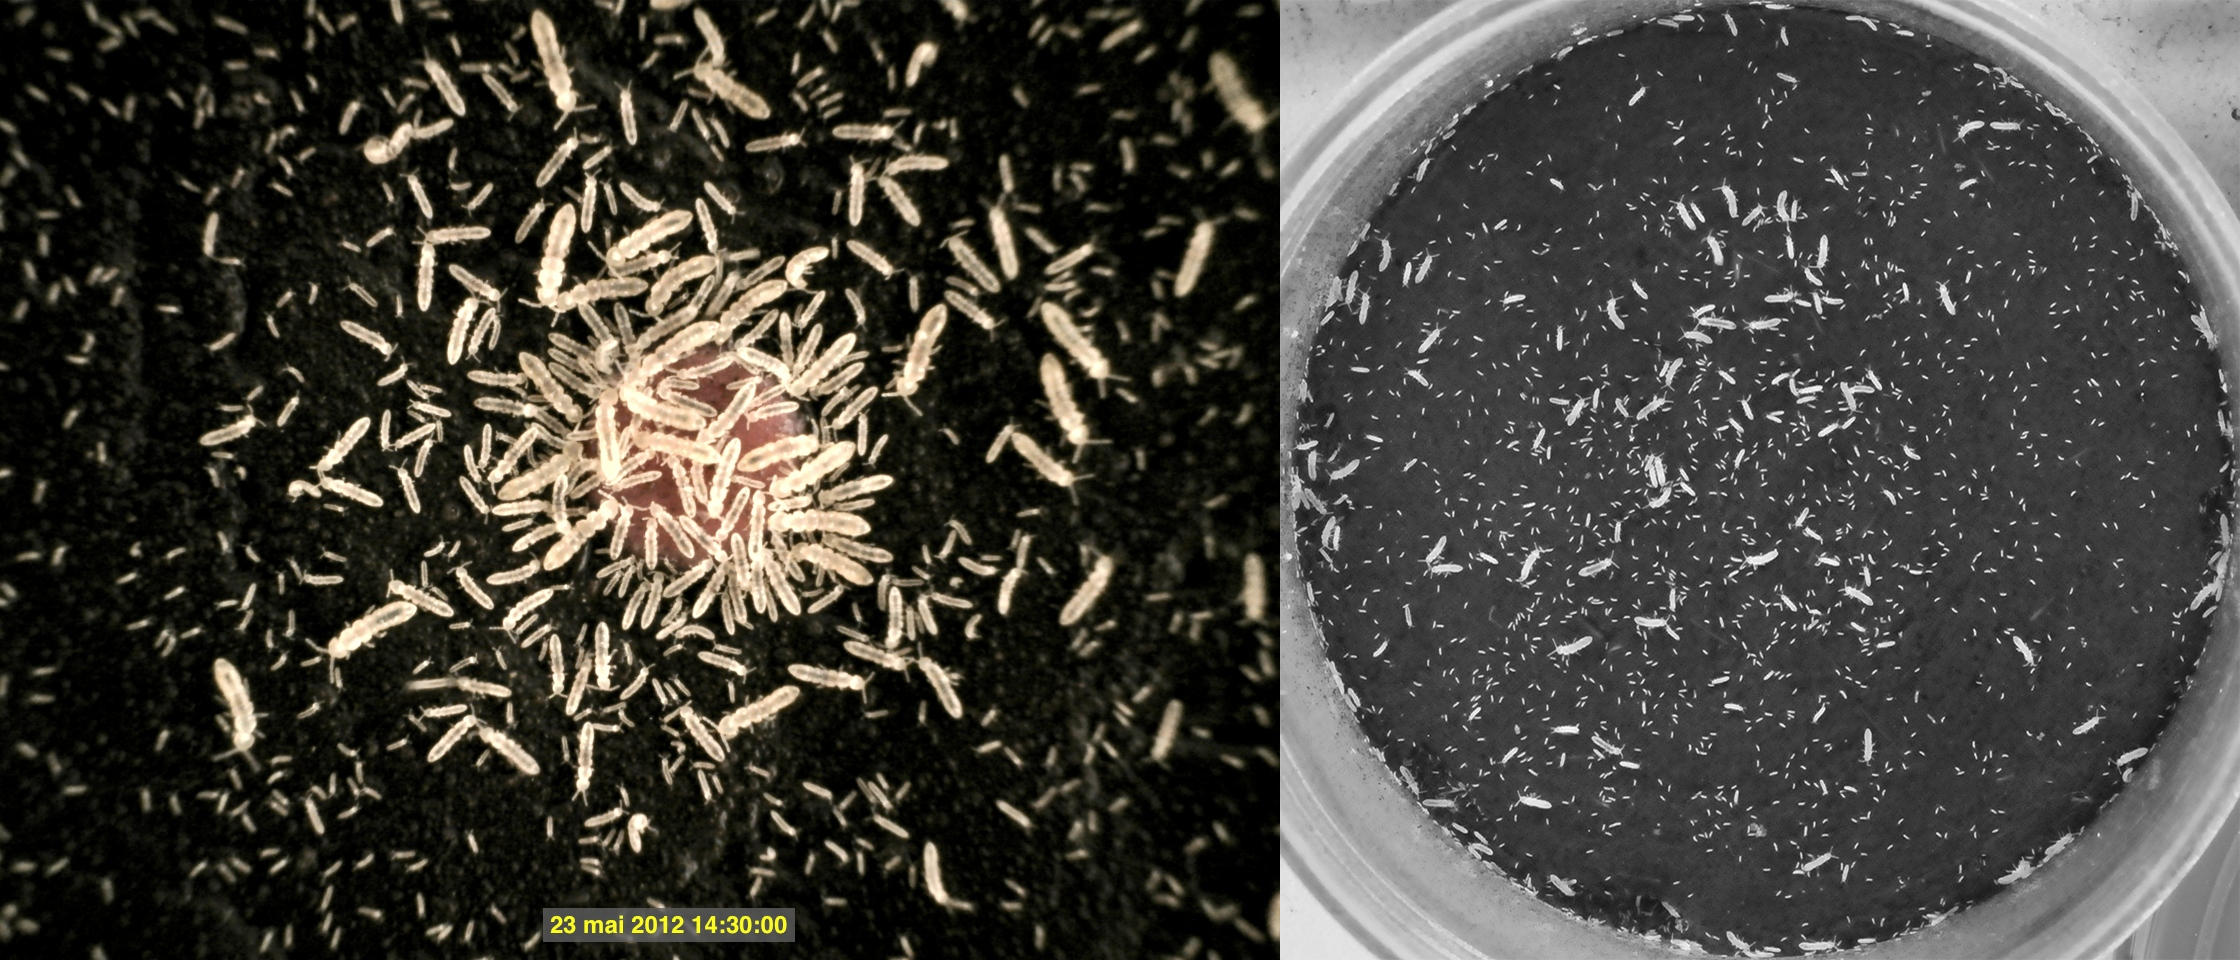
\includegraphics[width=1\textwidth]{1_CorpsDeThese/Resumes/Fig/SM05b}
\caption[\lofimage{1_CorpsDeThese/Resumes/Fig/SM05b}Cliché
d'observation de l'accès à la ressource]{Cliché
d'observation de l'accès à la ressource pour la population témoin HA-01 et
cliché de la population totale à une date proche.}
\label{fig:SM5}
\end{center}
\end{figure}

La Figure \ref{fig:SM5} montre un exemple de cliché pris au cours de
l'observation comportementale de l'accès aux ressources. Ce cliché a été pris
pour la population témoin HA 01. Bien que ce ne soit qu'un seul exemple de
cliché, cet exemple est très représentatif de ce qui a été observé dans toutes
les populations mesurées. On peut observer sur ce cliché une forte concentration
d'individus regroupés sur la pastille de nourriture (en rouge au centre) et des
individus plus dispersés aux alentours. Il est intéressant de constater la
différence de taille des individus sur ou aux abords de la pastille de ressource
comparée à la celle des individus plus éloignés et à l'ensemble des individus de
la population. Alors que les individus éloignés sont majoritairement des
juvéniles, les individus les plus gros présents sur ce cliché sont tous sur la
pastille de ressource ou dans ses environs proches.
Ceci est observé alors même qu'en nombre d'individus, cette population est
largement dominée par les juvéniles. Si l'accès à la ressource était indépendant
de la taille, on s'attendrait donc à avoir davantage de juvéniles présents sur
la pastille que de grands individus. Il y a donc un biais de taille corporel
manifeste dans l'accès à la ressource.

\begin{figure}[!ht]
\begin{center}
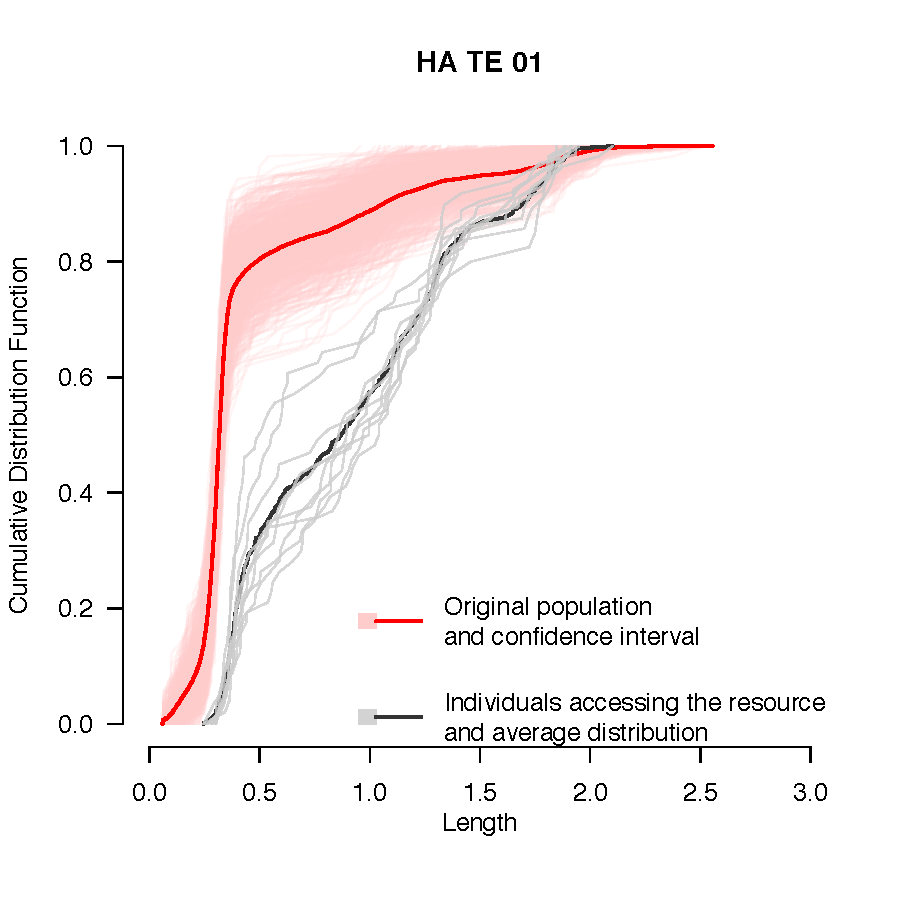
\includegraphics[width=0.75\textwidth]{1_CorpsDeThese/Resumes/Fig/SM06}
\caption[\lofimage{1_CorpsDeThese/Resumes/Fig/SM06}Mesure du biais
d'accès aux ressources]{Mesure du biais
d'accès aux ressources pour la population témoin HA 01. Test de
Kolmogorov-Smirnov de comparaison de deux échantillons: gris en dessous du
rouge: $p<10^{-10}$.}
\label{fig:SM6}
\end{center}
\end{figure}

Le cliché présenté en Figure \ref{fig:SM5} fait partie d'une série de 10 clichés
de la même population à 15 minutes d'intervalle. La Figure \ref{fig:SM6}
présente les fonctions de distribution cumulées de la population totale (rouge),
des individus accédant à la ressource sur chacun des clichés (gris clair), de la
moyenne des individus accédant à la ressource (gris foncé), et de 1000
échantillons aléatoires de même taille que la distribution moyenne des individus
accédant à la ressource (rouge clair). On constate que les dix distributions en
gris sont systématiquement en dessous de la distribution dans la population entière. Qui
plus est, elles sont également systématiquement en dehors de l'intervalle des
sous échantillons aléatoires. Le test de comparaison des distributions,
effectué avec la distribution moyenne sur la pastille est également extrêmement
significatif.
Cela nous permet d'affirmer qu'il y a un biais significatif en faveur des
individus les plus grands de la population dans l'accès à la ressource. En
effet, alors que $80\%$ des individus de la population mesurent moins de
$0.5mm$, ils ne représentent qu'un tiers des individus présents sur ou aux
abords de la pastille de nourriture. De plus, $13\%$ des individus sur la
ressource mesurent plus de $1.6mm$ alors qu'ils représentent moins de $5\%$ de
la population totale. Enfin, $50\%$ des individus présents sur la pastille ont
une taille entre $0.45$ et $1.35mm$ alors que cette classe de taille ne
constitue que $15\%$ de la population totale.

\subsubsection{Mesure du biais d'accès aux ressources}

La mesure du biais par comparaison des distributions cumulées a été réalisée sur
10 populations. La Figure \ref{fig:SM7} présente les distributions cumulées des
neufs autres séries d'observation.
On constate que dans tous les cas il existe un biais en faveur des individus les
plus grands pour l'accès à la ressource. On constate également que même dans les
populations où le nombre de grands individus est relativement important, telle
que TO TE 01, le biais reste significatif avec une large sous représentation des
$40\%$ d'individus de moins de $0.5mm$.

On remarque encore que même dans les populations où les juvéniles représentent
plus de $80\%$ de la population totale (HA JM 01, HA JM 02, HA TE 02, TO MG 02),
on ne comptabilise sur la ressource jamais plus de $50\%$ d'individus de moins
de $0.6mm$. Sur l'ensemble des cas étudiés, les $10\%$ les plus grands des
individus de la population totale représentent jusqu'à plus de $50\%$ des
individus mesurés sur les ressources, et généralement autour de$20\%$.

\begin{figure}[!ht]
\begin{center}
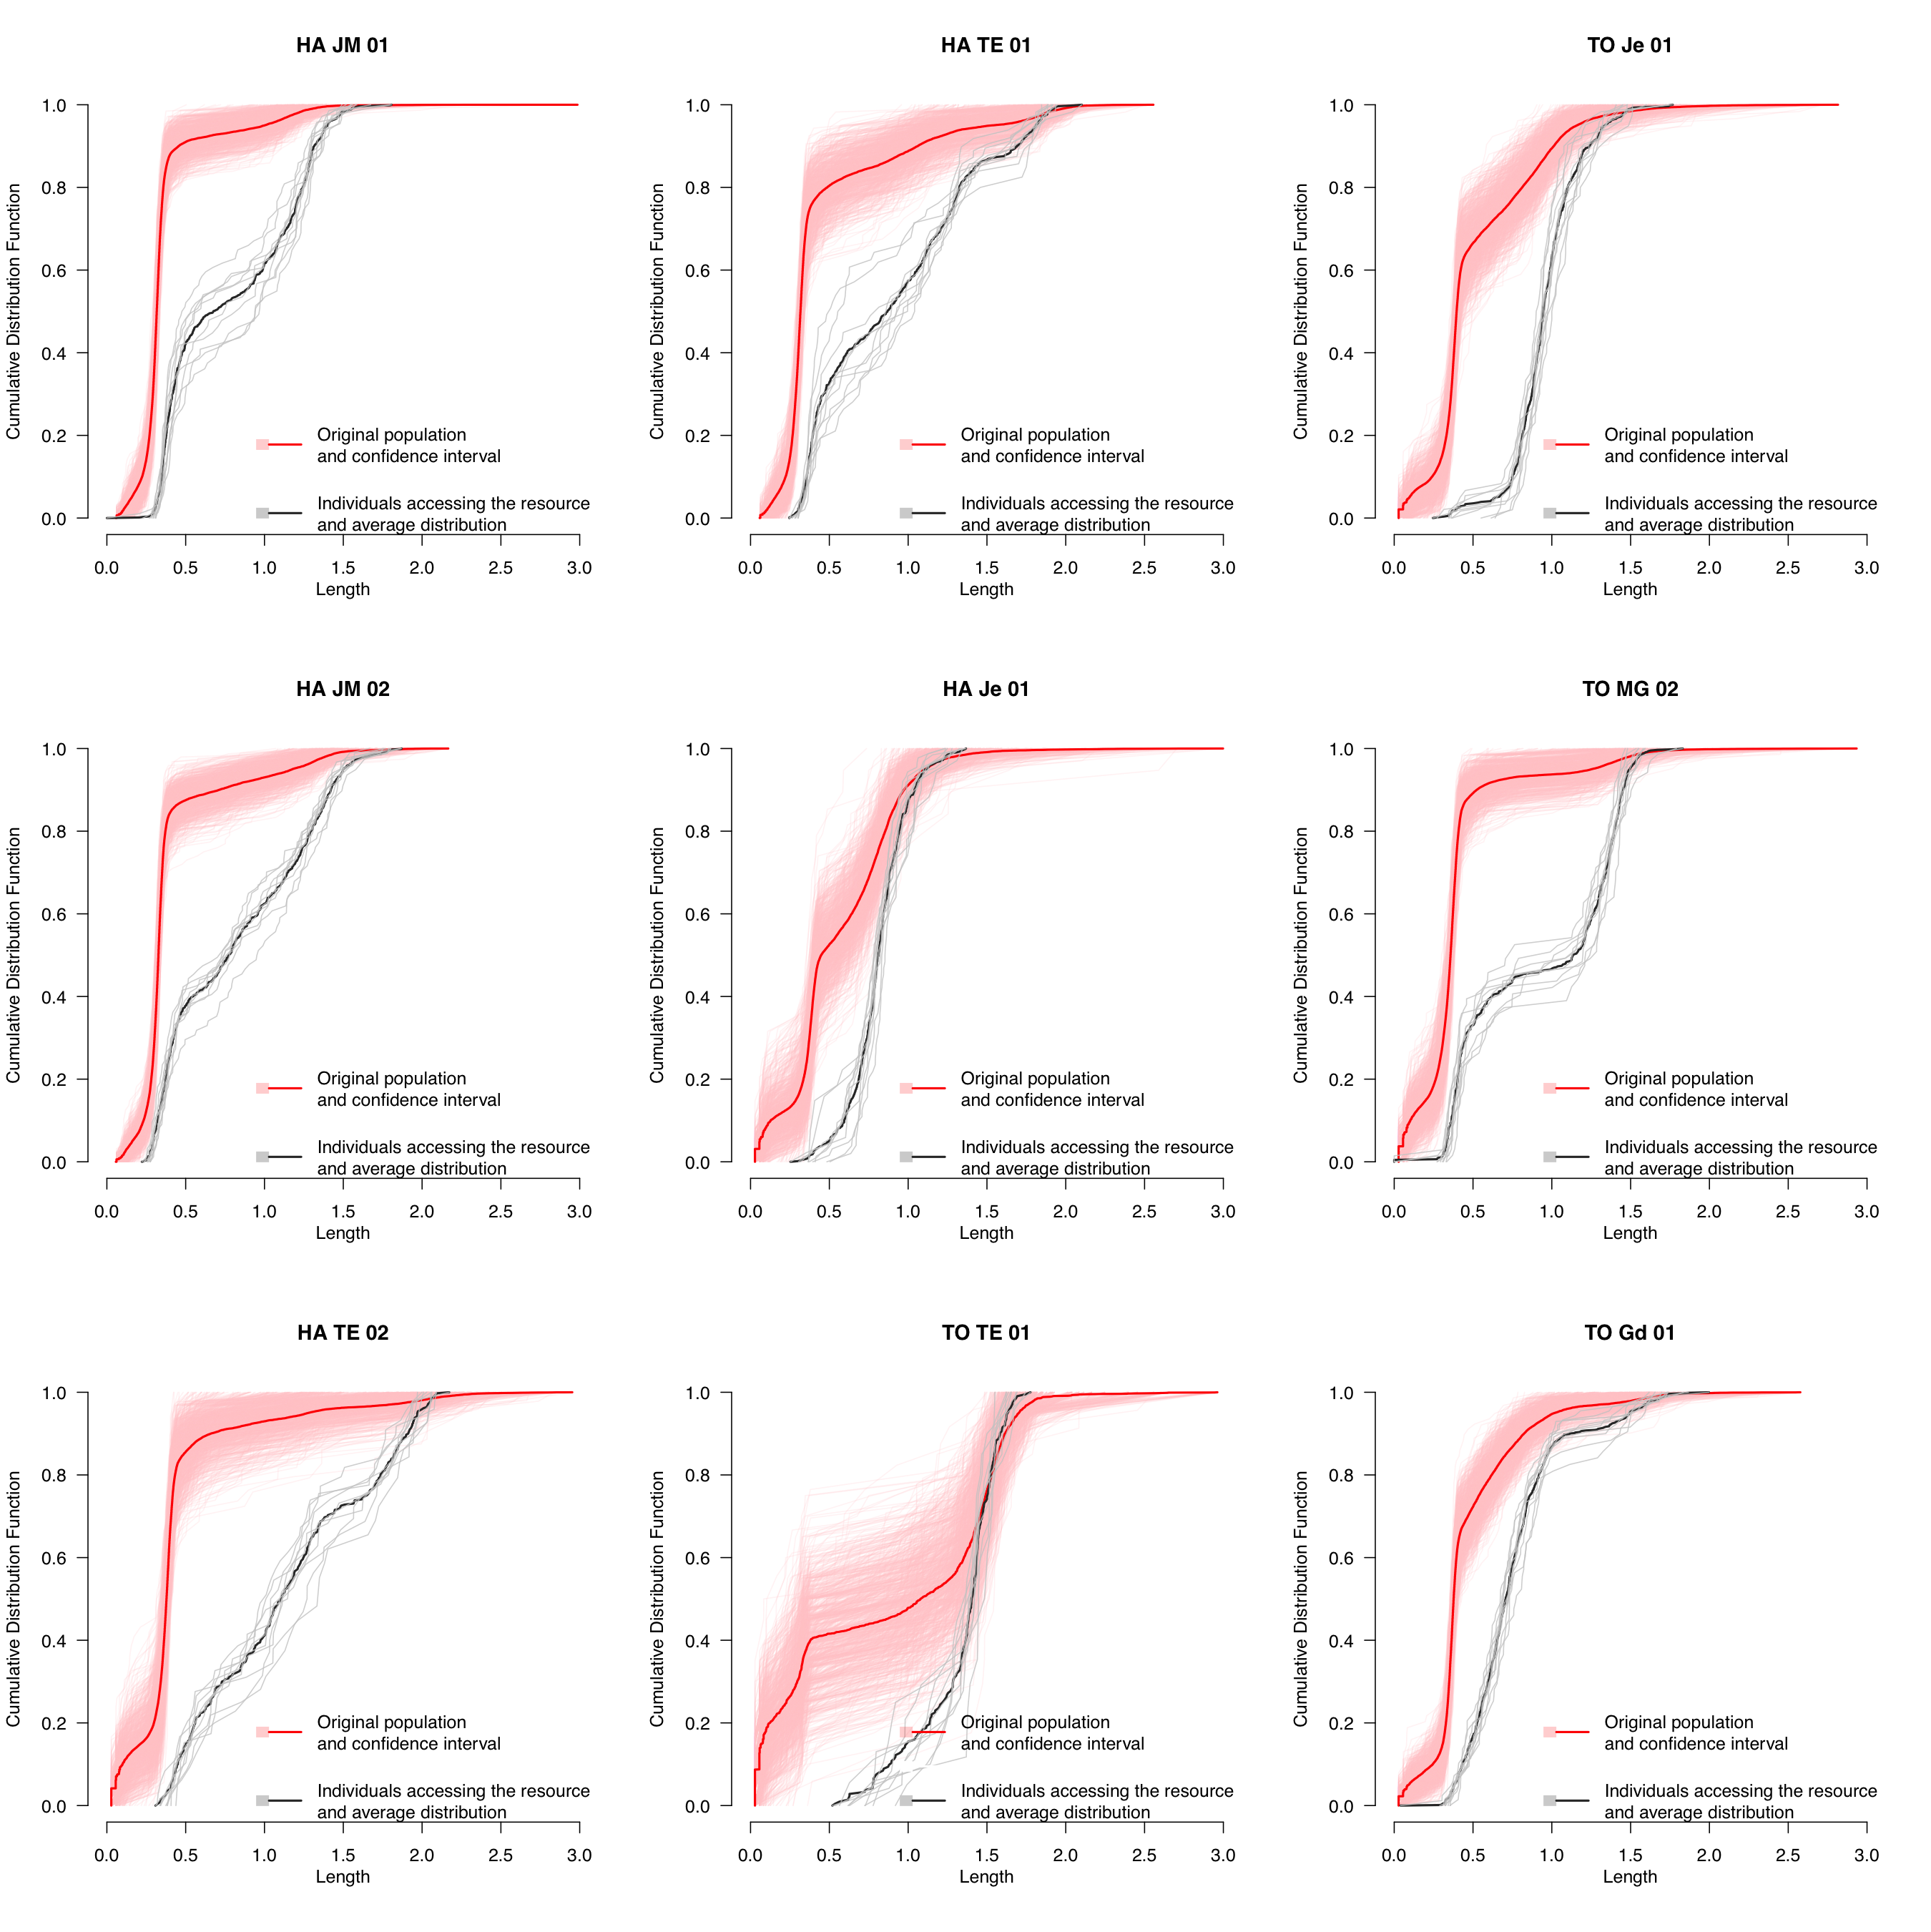
\includegraphics[width=1\textwidth]{1_CorpsDeThese/Resumes/Fig/SM07}
\caption[\lofimage{1_CorpsDeThese/Resumes/Fig/SM07}Mesures du biais
d'accès aux ressources]{Mesures du biais
d'accès aux ressources pour 9 autres populations. Tests KS: $p \ll 0.01$}
\label{fig:SM7}
\end{center}
\end{figure}

Les biais en faveur des grands individus dans l'accès à la ressource semblent
donc être systématiques, quelle que soit la population étudiée. Nous avons
utilisé dans ces observations des populations dont la structuration en taille était
différente.
Ainsi, même avec très peu de grands individus dans la population, ceux-ci sont
très largement sur-représentés lors des comptages sur les pastilles. Il semble
donc que la capacité des individus de grande taille à dominer la ressource soit
commune à nos deux clones, et ne dépende que peu des conditions de densité de la
population. Lors de la prise des clichés servant de base à ces mesures, nous
avons également pu identifier en temps réel des interactions
compétitives entre individus: des individus se
mettaient à tourner rapidement en rond lorsque d'autre s'approchaient de trop prêt, provoquant leur fuite. Ces comportements étaient
particulièrement visibles chez les individus les plus grands, faisant fuir
rapidement les plus petits. Ainsi, la
domination des plus grands individus sur la ressource passe notamment par des
comportements consistant à chasser les individus plus faibles de leur
environnement direct, empêchant les fuyards d'accéder à la ressource. Ce
comportement répond à notre définition précédente de la compétition par
interférence (Chapitres \ref{chap:method} et \ref{chap:amnat}, et Annexe
\ref{An:AmNat}).

\section{Discussion}

Au cours de cette étude, nous avons analysé la réponse de la structure en taille
de populations de collemboles à des perturbations. Plusieurs perturbations ont
été appliquées aux deux clones étudiés jusque là, HA et TO. Ces perturbations
ont consisté à manipuler la structure en taille de la population pour observer
l'établissement d'un nouvel équilibre en fonction des nouvelles conditions
imposées. 

Nous avons également réalisé une série d'observations des
comportements individuels d'accès aux ressources. Ces observations nous ont
permis de mettre en évidence un biais systématique dans l'accès à la ressource
en faveur des individus les plus grands de la population. 

\subsection{Stabilité et résilience des différentes structures en taille}

Au cours de la première expérience, nous avons manipulé la structure de
plusieurs populations des clones HA et TO. Les différentes manipulations
réalisées ont permis de tester la stabilité des différents attracteurs décrits
dans le Chapitre \ref{chap:sp}. En effet, les huit populations HA utilisées
dans l'étude étaient toutes dans une structure de type 4 au moment de la
perturbation, alors que les populations TO étaient dans des structures de type 1
ou 2. Nous avions déjà constaté que les structures de type 4 n'étaient stable
que le temps de survie des adultes les plus grands; une fois disparus,
ces derniers n'étaient pas remplacés et les populations convergeaient vers
différentes structures. Ceci est encore confirmé par nos populations HA témoins,
en effet, les adultes les plus grands survivent après le changement de boite
d'élevage mais meurent de vieillesse après quelques centaines de jours (voir
\autocites{mallard2013b} pour plus d'informations sur le vieillissement).
La structure observée subit alors le même type de transition que les populations présentées
dans le Chapitre \ref{chap:sp} (voir aussi Annexe \ref{Ann:SP}). De plus,
lorsque les adultes les plus grands sont retirés des populations, ils ne sont pas remplacés malgré une légère
croissance des adultes de taille intermédiaire. A la place, une cohorte de
juvéniles parvient à grandir et rejoint les adultes intermédiaires, augmentant
la compétition au sein de cette classe, ce qui empêche une croissance vers les
très grandes tailles. Enfin, lorsque l'on enlève les juvéniles ou les adultes
de taille intermédiaire, les plus grands parviennent à se maintenir quelques
temps après perturbation mais ne sont pas remplacés après leur mort. Cette
structure trimodale est donc stable localement, mais le bassin d'attraction est
trop petit pour permettre de l'atteindre, à part dans des conditions très
particulières telles que décrites dans le Chapitre \ref{chap:sp} (voir aussi
Annexe \ref{Ann:SP}).

A l'inverse, la plupart des populations dont la structure a été modifiée au
moment de la manipulation convergent vers une structure avec un grand nombre de
juvéniles, et des adultes plutôt petits et en assez forte densité. Cette
structure, similaire aux structures de type 1, semble donc avoir un bassin
d'attraction plus large que les autres car elle est atteinte quel que soit la
manipulation effectuée sur la structure. Cette structure est généralement
atteinte lorsque beaucoup de juvéniles grandissent et atteignent la maturité en
même temps. Au cours de nos différentes manipulations, soit des juvéniles
étaient présents et pouvaient grandir dès que la pression de compétition était
relâchée par le retrait de tout ou partie des adultes, soit seul des adultes
étaient gardés, mais ils se sont alors massivement reproduits et à cause d'une
faible compétition, une large cohorte de juvénile a pu rapidement commencer à
grandir et atteindre la maturité. 

On constate également que le temps nécessaire à la stabilisation d'une nouvelle
structure semble dépendre principalement de la présence ou de l'absence des
adultes. En effet, les populations les plus rapides à atteindre un équilibre
sont celles dont tous les adultes ont été prélevés (2 à 3 semaines).
A l'inverse, les plus lentes sont celles dont seuls les juvéniles ont été
prélevés ($>200$ jours). En diminuant la possibilité des juvéniles d'accéder à
la ressource, les adultes acquièrent une longue survie, ce qui fait d'eux une
force stabilisatrice de la structure, mais en ralentissant la capacité de
grandir des juvéniles, cela ralentie également la possibilité pour la population
de se remettre d'une perturbation et notamment du prélèvement de ses juvéniles.

\subsection{Compétition par interférence}

L'impact du retrait des adultes d'une population sur la reprise de croissance
des juvéniles, ainsi que le biais dans l'accès aux ressources en faveur des
individus les plus grands viennent confirmer l'hypothèse de la compétition par
interférence comme force régulatrice de la dynamique de nos populations de
collemboles. Cette interférence s'exprime principalement via des comportements
individuels lors de l'accès à la ressource. En effet, les individus ont tendance
à chasser leurs voisins lorsqu'ils sont trop proches. Au cours de cette
opération, les individus les plus grands parviennent à chasser la plupart de
leurs voisins alors que les plus petits ne les affectent pas. Au contraire, les plus petits
ont davantage tendance à fuir, et limitent ainsi leur accès à la ressource. De
ce fait, la présence, même en faible densité, d'individus très grands affecte
fortement la dynamique de la structure comme proposé par notre étude théorique
du Chapitre \ref{chap:amnat} (voir aussi Annexe \ref{An:AmNat}). En monopolisant
la ressource, ils bloquent la croissance des individus plus petits, et une nouvelle cohorte de juvénile ne
parvient à grandir que lorsque les adultes les plus grands ont disparu, comme
observé dans les premières expériences présentées ici, et dans le Chapitre
\ref{chap:sp} (voir aussi Annexe \ref{Ann:SP}).

En revanche, contrairement a ce qui est prédit par le modèle, la disparition
ou le retrait de la cohorte des individus les plus grands ne provoque pas sont
remplacement, mais plutôt un changement de dynamique car lors de cette
disparition, beaucoup de juvéniles se mettent à grandir en une fois, ce qui
modifie fortement les rapports de compétition entre les différentes cohortes et
au sein de chacune.

De plus, les résultats de ces expériences montrent également que la compétition
par exploitation continue de jouer un rôle dans la régulation des populations.
En effet, la suppression de l'ensemble des juvéniles, les individus les plus
compétitifs par exploitation, affecte les adultes, qui sont alors capables de
reprendre leur croissance jusqu'à l'éclosion de nouvelles cohortes de juvéniles.

\section{En conclusion}

Cette série d'expérience a permis de confirmer le rôle
prépondérant que jouent les adultes dans la régulation de la dynamique des
populations structurées de Collembole. Mais elle a également apporté des
arguments montrant l'existence d'une régulation par la compétition par
exploitation. Les deux mécanismes semblent donc intimement liés, et c'est
l'équilibre entre les deux qui conduit aux dynamiques observées dans le Chapitre
\ref{chap:sp} (voir aussi Annexe \ref{Ann:SP}). Un changement brutal de cet
équilibre en prélevant une partie de la population, diminuant rapidement l'impact de la compétition par interférence
(en retirant les adultes) ou par exploitation (en retirant les juvéniles)
affecte la population en la conduisant généralement vers un nouvel équilibre de
structure. 

L'équilibre entre compétition par interférence et compétition par exploitation
dans la régulation des populations structurées dépend de la structure de la
population elle même, mais est également susceptible de dépendre des conditions
environnementales. La température est un élément connu pour son impact sur la
taille des individus, et est donc susceptible d'affecter cet équilibre en venant
non seulement modifier les trajectoires d'histoire de vie individuelles, mais
également les interactions entre les individus et les mécanismes de densité
dépendance. Les interactions entre mécanismes de compétition et effets
de la température seront l'objet du chapitre suivant. 



\chapter{Interactions entre compétition intraspécifique et température dans la
régulation des populations structurées}
\chaptermark{Compétition intraspécifique et température}
\label{chap:fip}

\vspace{2cm}
\begin{Spacing}{1}
\texttt{
Mallard, François, Vincent Le Bourlot, Christie Le Coeur, Monique Avnaim, David
Claessen and Thomas Tully, "From individuals to populations: \\intraspecific
competition breaks the temperature-size rule"\\
soumis à Journal of Animal Ecology}
\end{Spacing}
Voir Annexe \ref{Ann:fip}.
\vspace{2cm}


\lettrine[lines=3]{A}{u cours} des trois chapitres précédents, nous avons étudié
le rôle des mécanismes de compétition intraspécifiques sur la dynamique de
populations structurées de collemboles \textit{Folsomia candida} d'un point de vu théorique
et empirique. Ces études nous ont permis en particulier de mieux appréhender
l'impact de différents niveaux de compétition par interférence dans la
dynamique temporelle de la structure des populations. Cependant, ces études ont
été réalisées dans une seule condition environnementale. Or, comme nous
l'avons déjà expliqué, l'environnement, et en particulier la température, peut
avoir un impact à la fois sur les individus et les populations. 

En effet, des températures différentes affectent directement les taux
physiologiques (métabolisme, consommation, respiration,\ldots), ce qui a des
conséquences démographiques via des changements dans les cycles de vie
\autocites{gillooly2002a,le-galliard2012a}. Des changements de température
provoquent aussi de la plasticité phénotypique chez les individus en modifiant
par exemple l'allocation des ressources à la croissance ou à la reproduction
\autocites{liefting2010temperature,gutteling2007mapping}. Ceci résulte dans la
règle dite ``taille-température'' qui prédit une taille plus grande des
individus dans des environnements plus froids
\autocites{atkinson1994a,atkinson1996a,angilletta2009a}. Enfin, la température
peut avoir un effet sur les comportements individuels comme l'activité, la
dispersion ou le choix de l'habitat
\autocites{atacho2013a,bonte2008thermal,vanbeest2012temperature}.

L'approche classique de l'étude de l'influence de la température sur les
phénotypes consiste à mesurer des normes de réaction \autocites{woltereck1909a}.
Ces mesures sont généralement réalisées sur des individus isolés ou sur de
petites cohortes élevées au laboratoire dans différentes conditions de
température. Ces analyses apportent beaucoup d'informations sur les effets au
niveau de l'individu mais laissent de côté les conséquences de ces effets aux
niveaux des populations et des communautés. 

Dans ce chapitre, nous nous demandons a quel point les normes de réactions
mesurées au niveau individuel permettent des inférences sur la dynamique des
populations. Nous cherchons à comprendre comment les effets directs de la
température sur les traits d'histoire de vie individuels sont modulés par les
interactions entre individus et les rétroactions démographiques.
Les effets d'une augmentation de la température sur la compétition
inter-spécifique ont déjà été démontrés, provoquant notamment une augmentation
de la compétition par exploitation \autocites{ohlberger2011a}. Mais le cas de la
compétition intra-spécifique reste peu clair, et les effets sur la compétition par
interférence peuvent être différents de l'exploitation. L'interaction entre
les deux mécanismes, couplée aux effets directes de la température sur les individus,
rendent l'impact de la température sur les dynamiques des populations
structurées difficile à prévoir. Pour y parvenir, nous avons mesuré les normes de réaction
individuelles des taux de croissance et des tailles à maturité et tailles
asymptotiques dans quatre conditions de température, $11$, $16$, $21$ et
$26\degres$C. Nous avons également effectué des mesures de taux de croissance de
cohortes et de taille des cohortes adultes dans des populations élevées aux même
températures. Nous avons ainsi pu comparer les réponses à la température dans
deux conditions démographiques contrastées et en déduire l'importance de la
compétition intra-spécifique dans la réponse des populations à la température.

\section{Éléments de méthodologie}

\subsection{Conditions d'élevage et mesures}

Comme dans les expériences précédentes, les conditions d'élevage et les méthodes
de mesure de la taille individuelle et de la structure des populations suivent
les descriptions données dans le Chapitre \ref{chap:method}.

\subsubsection{Individus isolés}

Les nouveau-nés sont isolés immédiatement après la naissance et sont nourris
\textit{ad libitum} pendant toute leur vie. Les individus ont été placés
aléatoirement à une des quatre températures de notre intervalle ($11$, $16$, $21$ et
$26\degres$C). La taille corporelle est mesurée pour chaque individu trois fois
par semaine pendant dix semaines, puis une fois par semaine. Afin de déterminer
la maturation des individus, les boites d'élevage sont régulièrement inspectées
pour rechercher des pontes. La croissance des individus est ensuite modélisée
\ref{fig:FIP1} et Annexe Figure \ref{Fig5-S1}).
Le taux de croissance maximal moyen et la taille asymptotique sont estimés par des modèles
de moindre-carrés non linéaires ajustés séparément pour chacune des trajectoires
de croissance \autocites{pinheiro2000a}. Les effets fixes du clone et de la
température (prise comme variable catégorielle) sur le taux de croissance
maximal et la taille asymptotique ont été testés à l'aide de modèles linéaires
et de test de Fisher.

\begin{figure}[!ht]
\begin{center}
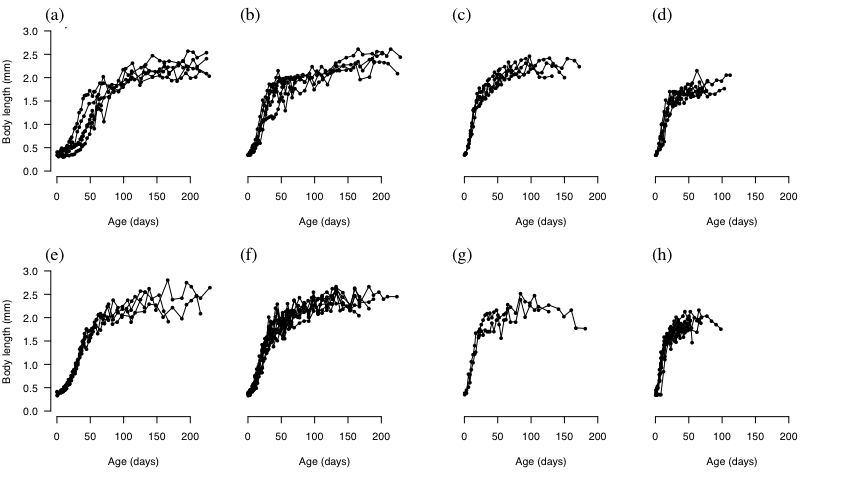
\includegraphics[width=\textwidth]{1_CorpsDeThese/Resumes/Fig/FIP01}
\caption[\lofimage{1_CorpsDeThese/Resumes/Fig/FIP01}Trajectoires de croissance
individuelles]{Trajectoires de croissance individuelles pour les clones HA
(a-d) et TO (e-h) à $11$ (a et e), 16 (b et f), 21 (c et g) et
$26\degres$C (d et h).}
\label{fig:FIP1}
\end{center}
\end{figure}


\subsubsection{Mesures de taille et de croissance dans les populations}

Pour les mesures de normes de réactions en contexte de population, quatre
populations ont été démarrées pour chaque température, excepté $21\degres$C où
les 28 populations présentées dans le Chapitre \ref{chap:sp} sont utilisées. La
structure des populations a été mesurée une fois par semaine pendant plus d'un
an. Les traits d'histoire de vie (taux de croissance des juvéniles et taille
adulte) ont été extraits des données grâce à la représentation en diagramme
structure-temps et aux outils annexes présentés dans le Chapitre
\ref{chap:method} Section \ref{sec:stdiag} (voir aussi Annexe \ref{Chap:STDiag}). 

Les taux de croissances juvéniles ont été mesurés sur des cohortes suffisamment
visibles sur les diagrammes et atteignant le groupe d'adultes (Figure
\ref{fig:FIP2} et Annexe Figure \ref{Fig5-S3}).
Le taux de croissance est estimé par la pente de la taille moyenne dans les cohortes au
cours du temps. La taille asymptotique des adultes est mesurée comme la taille
moyenne du groupe d'adultes une fois que la cohorte a totalement fusionné avec
les adultes déjà présents, ou quand sa taille moyenne se stabilise. La structure
de la population au moment de chaque mesure nous permet d'en connaître les
conditions démographiques (densité de juvéniles, d'adultes,\ldots). Les
individus sont considérés adultes lorsque leur taille excède $0.8mm$.

\subsubsection{Séparer les effets température et densité dépendance}

Dans nos populations, les changements dans les trais d'histoire de vie et les
taux démographiques peuvent être attribués à des effets directs de la
température sur les individus, à des effets directs des mécanismes de densité dépendance, ou
à une interaction entre les deux. Afin de pouvoir analyser les effets de la
densité dépendance (éventuellement en interaction avec la température) tout en
contrôlant pour les effets directs de la température, nous avons construit deux
indicateurs qui comparent les traits mesurés dans les populations aux mesures
faites sur les individus isolés. 

Pour analyser les différents effets sur le taux de croissance, nous avons
utilisé des modèles linéaires expliquant le rapport des taux de croissance dans
les populations sur les taux maximums moyens mesurés chez les individus isolés.
Nous appelons cet indicateur le ``\textbf{taux de croissance relatif en
population}''. Les variables explicatives que nous avons considérées sont le
logarithme du nombre d'adultes, la température, la lignée clonale et les
interactions entre les trois variables. 

\begin{figure}[H]
\begin{center}
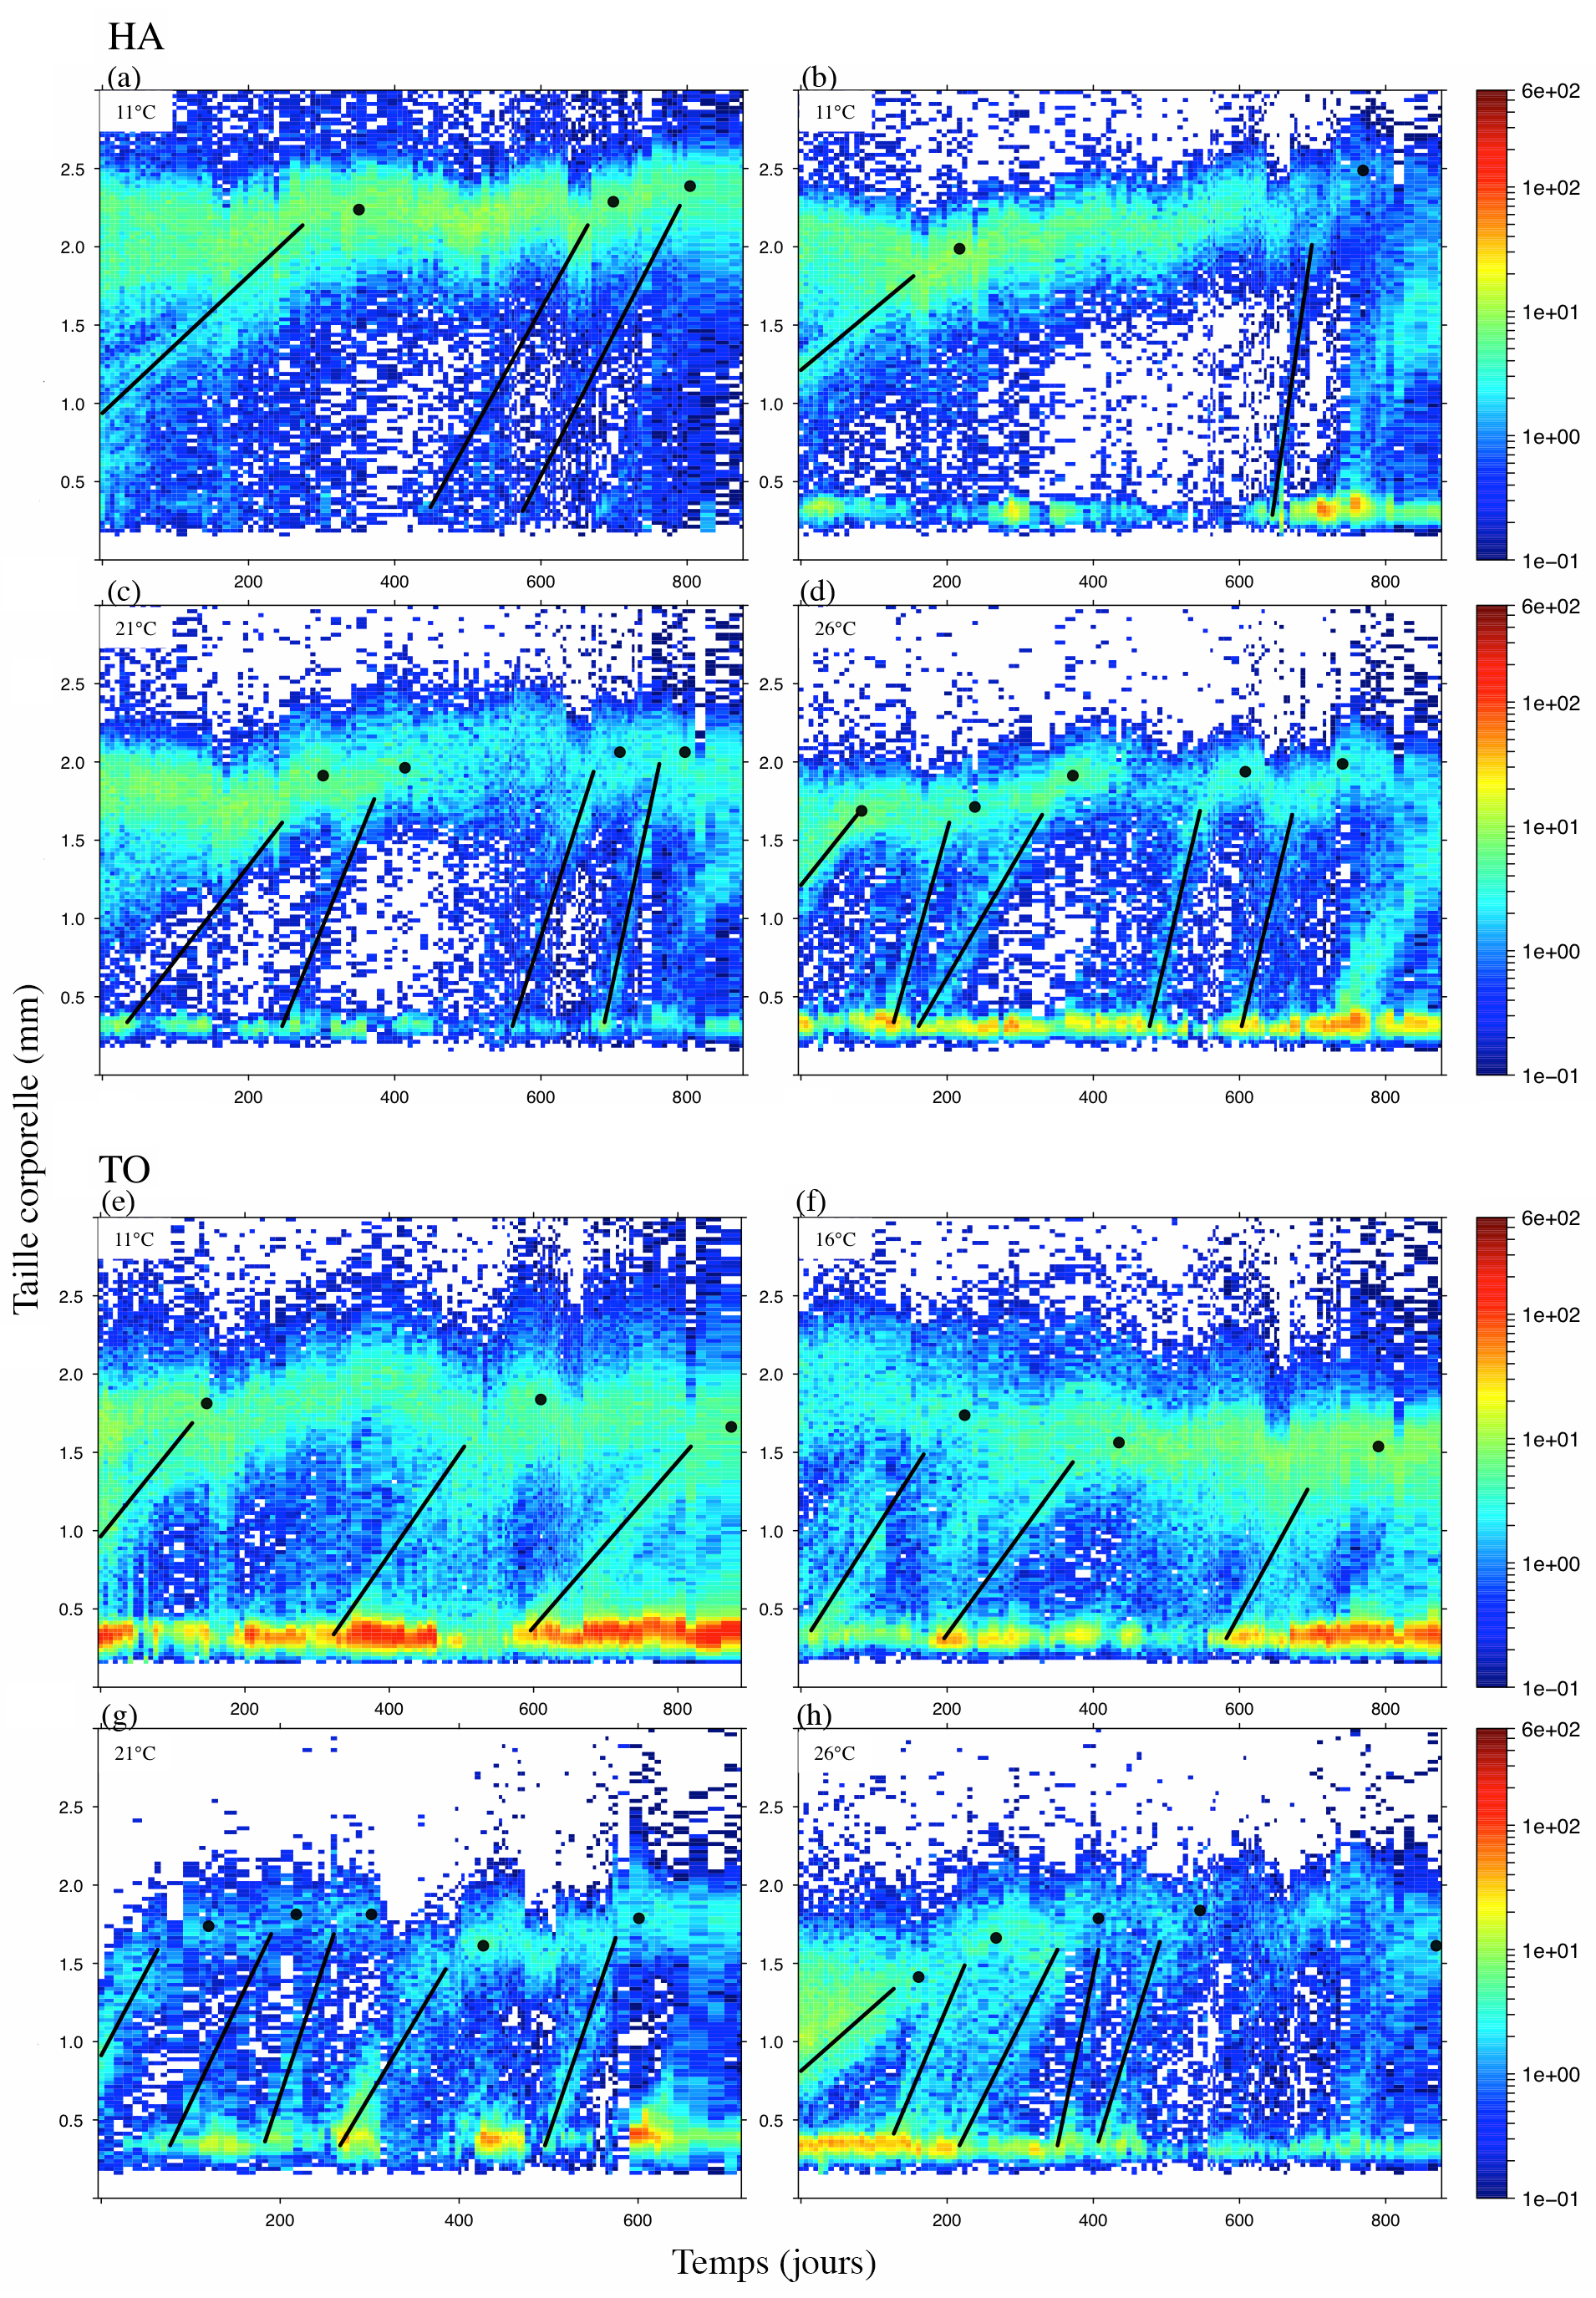
\includegraphics[width=\textwidth]{1_CorpsDeThese/Resumes/Fig/FIP02}
\caption[\lofimage{1_CorpsDeThese/Resumes/Fig/FIP02}Exemples de diagrammes
structures temps]{Exemples de diagrammes
structures temps pour les clones HA
(a-d) et TO (e-h) à $11$ (a et e), 16 (b et f), 21 (c et g) et $26\degres$C
(d et h). Les points noirs marquent les mesures de taille
adulte, tandis que les lignes marquent les mesures de
croissance de cohortes.}
\label{fig:FIP2}
\end{center}
\end{figure}

De la même façon, nous avons étudié la taille des adultes dans les populations
en la comparant aux mesures effectuées sur les individus isolés. Plus
précisément, nous avons construit un indicateur que nous appelons
``\textbf{l'effort de croissance au-delà de la maturité}'' ($GEBM$: ``Growth
Effort Beyond Maturation''). Cet indicateur représente l'investissement dans la
croissance après avoir atteint la maturité dans les populations comparé
à l'investissement en isolation. Il dépend de la température et se calculs comme
la proportion de croissance au-delà de la taille à maturité (mesurée en
isolation) comparée à la taille maximale mesurée en isolation:

\begin{equation}
GEBM(T) = \frac{Taille\ adulte_{populations}(T) -
Taille\ \grave{a} \ maturit\acute{e}_{isolation}(T)}{Taille\ adulte_{isolation}(T) -
Taille\ \grave{a} \ maturit\acute{e}_{isolation}(T)}
\end{equation}

A une température donnée, la taille à maturation et la taille maximale étant
connue pour les individus élevés en isolation, le $GEBM$ nous indique à quel
point un individu continue de croître après la maturation: $GEBM=0$ signifie que
les adultes stoppent leur croissance après la maturation, $GEBM=50\%$ qu'ils
atteignent une taille à mi-chemin de la taille asymptotique en isolation. Des
valeurs inférieures à 0 ou supérieures à $100\%$ signifie respectivement que les
adultes grandissent moins que la taille moyenne à maturité en isolation, ou
qu'ils grandissent plus que la taille maximale moyenne en isolation. N'ayant pas
trouvé de différence significative entre les deux clones, toutes les valeurs de
$GEBM$ ont été regroupées pour les analyses. Nous avons construit des modèles
linéaires avec comme variables explicatives la densité d'adultes, la
température et la lignée clonale avec toutes les interactions possibles. La
significativité des effets a été mesurées à l'aide d'ANOVA et de tests de
Fisher.

\section{Résultats}

\subsection{Norme de réactions à la température}

\subsubsection{Taux de croissance}

\begin{figure}[!ht]
\begin{center}
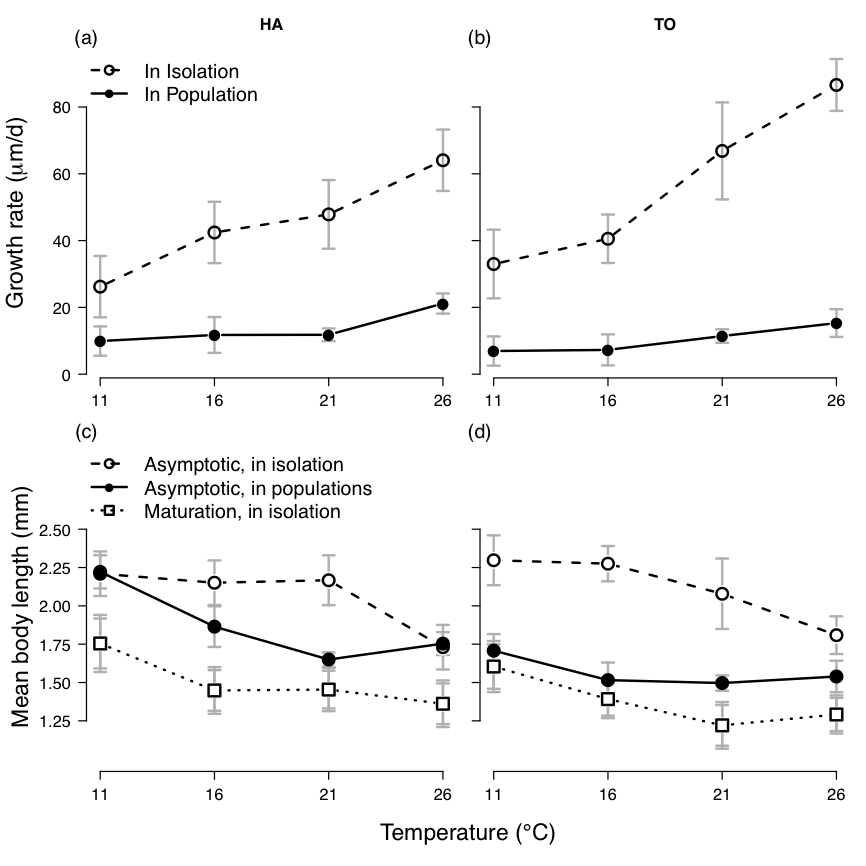
\includegraphics[width=0.95\textwidth]{1_CorpsDeThese/Resumes/Fig/FIP03}
\caption[\lofimage{1_CorpsDeThese/Resumes/Fig/FIP03}Normes de réactions des taux
de croissance et tailles moyennes]{Normes de réactions des taux de croissance (a
et b, moyennes et intervalles de confiance à $95\%$) pour les clones HA (a) et TO (b) mesurés en isolation (tirets) et sur les cohortes en condition de population (lignes pleines). Normes
de réaction de la taille corporelle (c et d): taille moyenne à maturité
(pointillés) et taille asymptotique des individus isolés (tirets) comparés à la
taille adulte moyenne en populations (lignes pleines).}
\label{fig:FIP3}
\end{center}
\end{figure}

La Figure \ref{fig:FIP3} représente les taux de croissance et les différentes
tailles mesurées en isolation ou en populations pour les deux clones. On peut
observer qu'en isolation, le taux de croissance individuel augmente quasiment
linéairement avec la température chez les deux clones (Figure \ref{fig:FIP3}a
et b). A $11\degres$C, les taux de croissance ne sont pas différents entre HA et
TO. Mais le taux de croissance augmente plus vite avec
la température chez TO que chez HA. Il en résulte à
$26\degres$C un taux de croissance $25\%$ supérieur chez TO par rapport à HA. 

Dans les populations, les taux de croissance mesurés sont beaucoup plus faibles
qu'en isolation (Figure \ref{fig:FIP3}a et b). En moyenne, il semble que les
juvéniles du clone HA grandissent plus vite que ceux de TO, mais l'effet de la
température sur les taux de croissance est le même pour les deux clones. 

\subsubsection{Tailles à maturité et taille asymptotique}

Chez les deux clones, les individus isolés suivent quasiment les mêmes normes de
réaction à la température, que ce soit pour la taille asymptotique ou pour la
taille à maturité (Figure \ref{fig:FIP3}c et d). Comme prédit par la règle
taille-température, la taille asymptotique diminue avec la température pour les
deux clones, sans différence significative entre eux. De plus, à part à
$11\degres$C où HA mature légèrement plus grand que TO, la taille à maturité
diminue avec la température de façon similaire pour les deux clones. 

Contrairement aux individus isolés, l'effet de la température sur la taille
moyenne des adultes en condition de population est différent pour les deux
clones. A $11\degres$C, les cohortes du clone HA atteignent en population une
taille qui n'est pas significativement différente de la taille asymptotique en
isolation (Figure \ref{fig:FIP3}c). Puis cette taille adulte moyenne décroît
progressivement pour être proche de la taille à maturité à une température de $21\degres$C. Mais de façon
beaucoup plus étonnante, la taille moyenne des adultes dans les populations du
clone HA ré-augmente entre 21 et $26\degres$C. 

Chez le clone TO à $11$ et $16\degres$C, les cohortes dans les populations
s'arrêtent de grandir peu de temps après avoir atteint leur taille à maturité
attendue d'après les mesures en isolations. Entre $16$ et $26\degres$C, la
taille moyenne des adultes reste statistiquement constante à une valeur intermédiaire
entre la taille à maturité et la taille asymptotique, toutes deux mesurées en
isolation (Figure \ref{fig:FIP3}d).

\subsection{Densité dépendance et température}

\begin{table}[!b]
\centering
\caption{\label{tab:FIP1}Résultats du modèle pour le taux de croissance relatif
des cohortes de juvéniles dans les populations.}
\scriptsize
\begin{tabular}{rccccl}
\hline 
\multicolumn{6}{c}{$lm(\text{taux de croissance} \sim (\log(\text{Densité
d'adultes}) + \text{Température}) * \text{Clone})$} \\
&&&&&\\
& Estimation & Erreur standard & Valeur $t$ & $\text{Pr}(>|t|)$ & \\
\hline

Intercepte = Clone HA, Température 11 & $1.22e+00$ & $8.59e-02$ & $1.42e+01$
& $<2e-16$ & $***$\\

$\log(\text{Densité d'adultes})$ & $-1.48e-01$ & $1.34e-02$ & $-1.10e+01$ & $<
2e-16$ & $***$\\

$\text{Température}$ & $-1.57e-02$ & $1.82e-03$ & $-8.60e+00$ & $8.61e-15$ & $***$\\

$\text{CloneTO}$ & $-4.90e-01$ & $1.18e-01$ & $-4.15e+00$ & $5.56e-05$ & $***$\\

$\log(\text{Densité d'adultes}):\text{CloneTO}$ & $6.79e-02$ & $1.86e-02$ & $3.65e+00$ &
$3.61e-04$ & $***$\\

$\text{Température}:\text{CloneTO}$ & $5.24e-03$ & $2.63e-03$ & $2.00e+00$ &
$4.79e-02$ & $*$\\

\hline 
\end{tabular} 
\end{table}

Pour comprendre les différences entre les normes de réaction mesurées sur les
individus isolés et sur les cohortes en populations, nous avons étudié la
réponse à la température et à la densité de nos deux indicateurs, le taux de
croissance relatif et le $GEBM$, et ce pour les deux lignées clonales. Nous
avons utilisé la densité d'adultes dans les populations comme mesure de densité
car les adultes représentent en moyenne $90\%$ de la biosurface totale des
populations, et nous avons pu démontrer leur rôle prépondérant dans la dynamique
des populations structurées (voir Chapitres \ref{chap:sp} à \ref{chap:sm} et
Annexes \ref{Ann:SP} et \ref{An:AmNat}).

\subsubsection{Taux de croissance relatif}

\begin{figure}[!ht]
\begin{center}
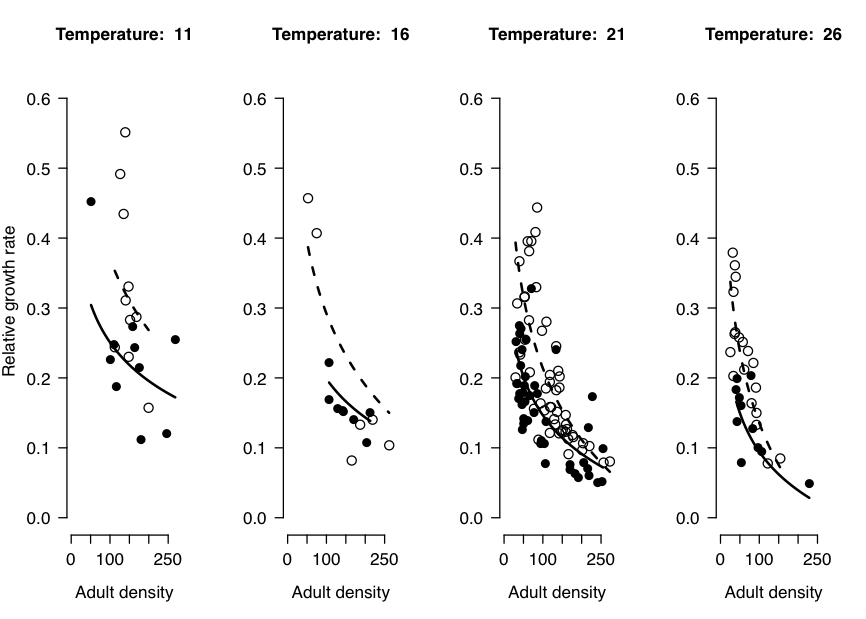
\includegraphics[width=\textwidth]{1_CorpsDeThese/Resumes/Fig/FIP04}
\caption[\lofimage{1_CorpsDeThese/Resumes/Fig/FIP04}Taux de croissance
relatifs]{Taux de croissance relatifs en fonction de la densité d'adultes dans
les populations pour les clones HA (lignes tiretées et symboles ouverts) et TO
(lignes pleines et symboles pleins)}
\label{fig:FIP4}
\end{center}
\end{figure}

A chaque température, le taux de croissance des cohortes de juvéniles dans les
populations diminue avec la densité d'adultes en suivant une loi exponentielle
(Figure \ref{fig:FIP4}, Table \ref{tab:FIP1}). En moyenne, les juvéniles des
populations du clone HA grandissent plus vite que ceux du clone TO, mais l'effet
délétère de la densité d'adulte y est également plus fort. Les différences
génétiques entre les clones ont donc tendance à s'atténuer avec la densité. 

L'augmentation de la température a également tendance à réduire le taux de
croissance relatif des cohortes. Cet effet est légèrement plus intense pour HA,
mais cela est probablement dû à un taux de croissance plus élevé que TO à
faible densité. 

\subsubsection{Effort de croissance après maturation}

\begin{figure}[!ht]
\begin{center}
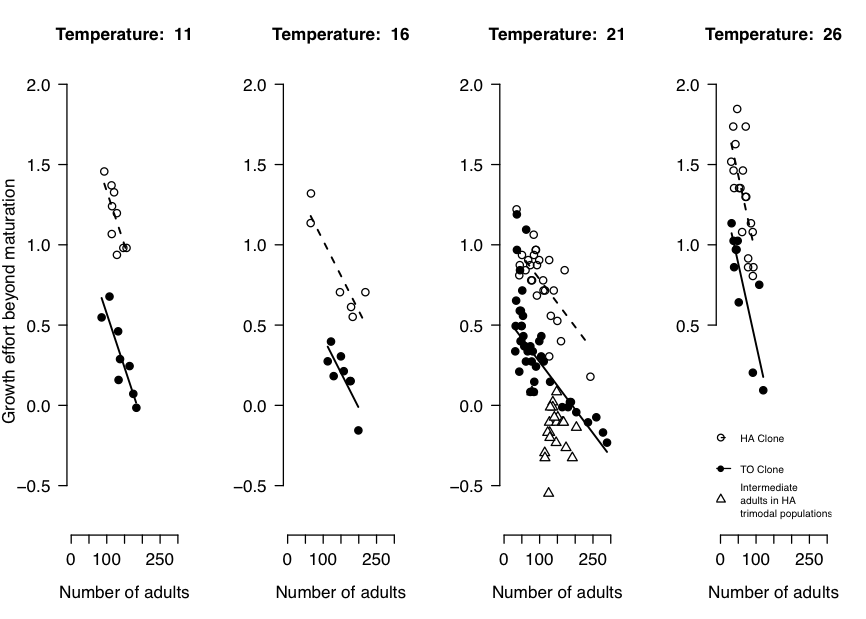
\includegraphics[width=\textwidth]{1_CorpsDeThese/Resumes/Fig/FIP05}
\caption[\lofimage{1_CorpsDeThese/Resumes/Fig/FIP05}GEBM]{Effort de croissance
après maturité ($GEBM$) en fonction de la densité d'adultes pour les quatre
températures. }
\label{fig:FIP5}
\end{center}
\end{figure}

La plupart des populations étudiées possèdent une structure bimodale similaire à
celles décrites dans le Chapitre \ref{chap:sp} (voir aussi Annexe \ref{Ann:SP}).
Cela permet de discriminer les adultes des juvéniles (voir Supplementary Materials de l'Annexe \ref{Ann:fip})
et ainsi d'estimer la densité et la taille moyenne des adultes afin d'estimer le
$GEBM$. La Figure \ref{fig:FIP5} montre que les réponses du $GEBM$ à la
densité et à la température diffèrent quantitativement mais pas qualitativement
entre les deux lignées (voir aussi Table \ref{tab:FIP2}). En moyenne, le $GEBM$
de HA est supérieur à celui de TO, indépendamment de la température. Cependant,
les différences entre clones s'atténuent avec la température. Pour chaque clone,
le $GEBM$ est négativement corrélé à la densité d'adultes: plus la densité
d'adultes est grande, plus leur taille moyenne se rapproche de la taille à
maturité mesurée sur les individus isolés à la même température. La pente de
cette corrélation et la même pour les deux clones à chaque température et donne
une mesure de la dépendance à la densité. 

\begin{table}
\centering
\caption{\label{tab:FIP2}Résultats du modèle pour le taux de croissance relatif
des cohortes de juvéniles dans les populations.}
\scriptsize
\begin{tabular}{rccccl}
\hline 
\multicolumn{6}{c}{$lm(GEBM \sim (\text{Densité
d'adultes} + \text{Clone}) * \text{Température})$} \\
&&&&&\\
& Estimation & Erreur standard & Valeur $t$ & $\text{Pr}(>|t|)$ & \\
\hline

Intercepte = Clone HA, Temperature11 & $2,01E+00$ & $1,93E-01$ & $1,04E+01$ & $<
2e-16$ & $*** $\\
Température16 & $-5,43E-01$ & $2,43E-01$ & $-2,23E+00$ & $2,77E-02$ & $* $\\
Température21 & $-9,25E-01$ & $1,98E-01$ & $-4,68E+00$ & $8,18E-06$ & $*** $\\
Température26 & $-7,06E-02$ & $2,10E-01$ & $-3,37E-01$ & $7,37E-01$ & $ $\\
Densité d'adultes & $-6,72E-03$ & $1,50E-03$ & $-4,48E+00$ & $1,84E-05$ & $*** $\\
CloneTO & $-7,62E-01$ & $7,88E-02$ & $-9,68E+00$ & $< 2e-16$ & $*** $\\
Densité d'adultes:Temperature16 & $2,35E-03$ & $1,77E-03$ & $1,33E+00$ & $1,87E-01$ & $ $\\
Densité d'adultes:Temperature21 & $3,76E-03$ & $1,53E-03$ & $2,46E+00$ & $1,56E-02$ & $* $\\
Densité d'adultes:Temperature26 & $-3,34E-03$ & $1,91E-03$ & $-1,75E+00$ & $8,36E-02$ & $. $\\
Température16:CloneTO & $1,58E-01$ & $1,15E-01$ & $1,37E+00$ & $1,73E-01$ & $
$\\
Température21:CloneTO & $2,48E-01$ & $8,80E-02$ & $2,82E+00$ & $5,71E-03$ & $**
$\\
Température26:CloneTO & $2,13E-01$ & $9,93E-02$ & $2,15E+00$ & $3,39E-02$ & $*
$\\

\hline 
\end{tabular} 
\end{table}

Comme observé au cours du Chapitre \ref{chap:sp} (voir aussi Annexe
\ref{Ann:SP}), certaines populations du clone HA à $21\degres$C exhibent une structure trimodale avec deux groupes d'adultes
stabilisés à des tailles différentes. Nous pouvons dès lors calculer le $GEBM$
indépendamment pour les deux groupes d'adultes.
Dans ces populations, nous avons trouvé un $GEBM$ très différents pour les deux
groupes d'adultes (Figure \ref{fig:FIP6}). Alors que les adultes les plus grands
ont un $GEBM$ qui suit le même modèle général que pour les autres populations,
le $GEBM$ des adultes les plus petits n'est pas expliqué par le nombre total
d'adultes dans les populations. Nous n'avons pas non plus trouvé de corrélation
significative entre le nombre d'adultes de petite taille et leur $GEBM$. En
revanche, à la fois le nombre d'adultes de petite taille et leur taille moyenne
sont corrélés au nombre d'adultes de plus grande taille. Nous avons donc
modélisé le $GEBM$ de tous les groupes d'adultes du clone HA à $21\degres$C à
l'aide du nombre d'adultes de plus grande taille (ou du nombre total d'adultes
pour les structures bimodales). Il est intéressant de constater qu'il n'y a
alors pas de différence significative dans la pente de la régression entre le
$GEBM$ des adultes de grande taille et celui des plus petits, seulement dans
leur intercepte (Figure \ref{fig:FIP6}). Dans les populations trimodales, la
présence d'adultes de grande taille agit donc sur le $GEBM$ des plus petits de
la même façon que si les populations étaient bimodales avec des petits adultes,
mais en densité supérieure ($260$ adultes de plus, voir Figure \ref{fig:FIP6}).

\begin{figure}[!ht]
\begin{center}
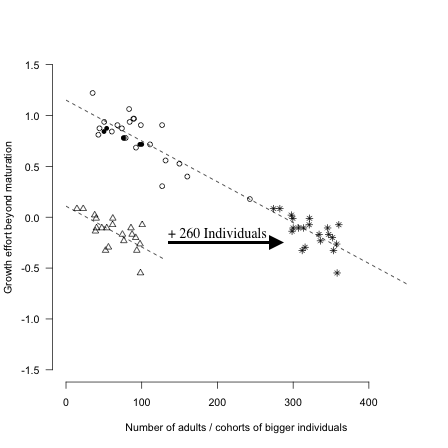
\includegraphics[width=0.75\textwidth]{1_CorpsDeThese/Resumes/Fig/FIP06}
\caption[\lofimage{1_CorpsDeThese/Resumes/Fig/FIP06}GEBM dans les
populations HA à $21\degres$C]{GEBM dans les
populations HA à $21\degres$C pour les adultes de petite taille ($\triangle$) et
de grande taille ($\circ$) dans les populations trimodales, et pour les petits
adultes s'il y avait 260 petits adultes de plus à la place des grands ($\ast$).}
\label{fig:FIP6}
\end{center}
\end{figure}

\subsubsection{Normes de réaction à la température des indicateurs}

L'indicateur $GEBM$ dépend également de la température pour nos deux lignées
clonales. Cependant, contrairement au taux de croissance relatif, l'effet de la
température sur $GEBM$ n'est pas linéaire. Afin d'étudier l'effet de la
température sur nos deux indicateurs en contrôlant pour l'effet de la densité au
sein de chacun des clones, nous avons tracé les taux de croissance relatifs et
$GEBM$ prédits pour une densité de 100 adultes en utilisant les modèles ajustés
pour chaque lignée indépendamment (Figure \ref{fig:FIP7a}). 

\begin{figure}[!ht]
\begin{center}
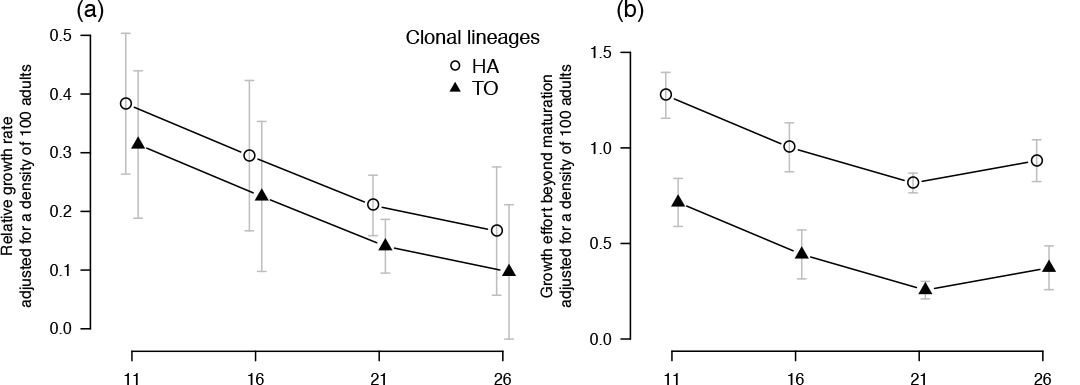
\includegraphics[width=0.75\textwidth]{1_CorpsDeThese/Resumes/Fig/FIP07a}
\caption[\lofimage{1_CorpsDeThese/Resumes/Fig/FIP07a}Normes de réaction
prédites à la température]{Normes de réaction à la température prédites pour
une densité de 100 adultes. (a) Taux de croissance relatif. (b) Effort de
croissance après maturation.}
\label{fig:FIP7a}
\end{center}
\end{figure}

Dans les deux lignées génétiques, le taux de croissance relatif décroît
linéairement avec la température (Figure \ref{fig:FIP7a}a), mais la norme de
réaction de $GEBM$ suit une forme en U: $GEBM$ décroît entre $11$ et
$21\degres$C mais augmente ensuite jusqu'à $26\degres$C (Figure
\ref{fig:FIP7a}b). Cette augmentation de $GEBM$ à la température la plus chaude
testée est remarquable car dans la plupart des populations élevées à $26\degres$C, la
taille adulte moyenne est plus grande que la taille asymptotique mesurée sur les
individus isolés à la même température (Figure \ref{fig:FIP5} à $21$ et
$26\degres$C), alors qu'à $21\degres$C chez HA, certaines cohortes n'atteignent
pas la taille à maturité mesurée en isolation (Figure \ref{fig:FIP5} à
$21\degres$C, valeurs négatives).

\section{Discussion}

\subsection{Normes de réaction des individus isolés}

Les normes de réactions mesurées sur des individus isolés montrent que les
Collemboles de l'espèce \textit{Folsomia candida} suivent la règle dite
``taille-température'' \autocites{atkinson1994a,angilletta2009a}. En effet,
dans des conditions froides, les individus grandissent plus lentement mais
atteignent des tailles supérieures à des individus isolés élevés dans des
conditions plus chaudes \autocites{angilletta2003a}. Bien que des études aient
déjà montré des effets similaires de la température sur les taux de croissance
de collemboles juvéniles \autocites{birkemoe2000a, driessen2007a, ellers2008a,
ellers2011b} ou sur la taille à maturité \autocites{stam1996a}, cette étude est
à notre connaissance la première à démontrer expérimentalement un ajustement
plastique de la taille adulte à différentes conditions de température ambiante.
Malgré des stratégies démographiques différentes entre les deux clones étudiés
\autocites{tully2008a,tully2011a}, les différences génétiques entre les clones
n'entraînent que très peu de différence dans les normes de réaction
individuelles à la température de la taille adulte, ce qui est similaire à ce
qui a déjà été observé chez un autre Collembole \autocites{driessen2007a}.

\subsection{Densité dépendance dans les populations}

Cette étude expérimentale constitue à notre connaissance la première description
expérimentale quantitative de dynamiques de populations structurées en taille le
long d'un gradient de température relativement large. Ces populations ont
généralement une structure bimodale avec un mode d'adultes et un mode de
juvéniles distincts. La plupart du temps, les juvéniles ne montrent pas de
croissance visible, mais un groupe de juvéniles parvient périodiquement à
grandir et recruter chez les adultes 

Que ce soit pour les taux de croissance ou les taille adultes, les normes de
réactions à la température en conditions de population sont différentes de
celles mesurées sur les individus isolés, avec des valeurs en moyenne plus
basses en population, probablement à cause de la compétition à l'\oe{}uvre pour
l'accès aux ressources (voir les Chapitres précédents). Dans nos populations,
l'apport de ressource est le même quel que soit la température ambiante. Les
populations atteignent donc un équilibre dynamique où la quantité de ressource
disponible limite le nombre, la taille corporelle et l'investissement
reproductif des adultes. Les équilibres atteints par les populations résultent
de rétroactions complèxes entre des stratégies démographiques
\autocites[dépendantes des clones,][]{tully2008a,stam1996a} et les effets de la
densité dépendance \autocites{kokko2007a} qui proviennent principalement de deux
mécanismes: la compétition pour la nourriture et pour l'espace. 

Comme montré dans les Chapitres précédents, la compétition pour la nourriture
est un des facteurs principaux de régulation de la dynamique de
nos populations de Collemboles. Cette compétition régule également les taux de
croissance des cohortes de juvéniles et les tailles corporelles atteintes par
les adultes (voir Chapitres \ref{chap:sp}, \ref{chap:amnat}, \ref{chap:sm} et
Annexes \ref{Ann:SP} et \ref{An:AmNat}).
Les effets négatifs de la densité sont visibles à deux échelles: (i) en
comparant les traits mesurés en populations aux traits mesurés sur des individus
isolés; et (ii) en comparant les traits mesurés dans des populations avec
différentes densités d'adultes. Nous avons montré dans cette étude que l'effet
négatif de la densité sur les traits d'histoire de vie peut être très fort (les
taux de croissance en population n'atteignent par exemple que 20 à $30\%$ des
valeurs mesurées sur des individus isolés). Cet effet de densité prend alors le
pas sur la plupart des ajustements plastiques dont les individus sont capables à
différentes températures. 

La comparaison des deux clones étudiés a permis de mettre en évidence des
différence génétiques significatives dans l'intensité de la densité dépendance:
pour les deux traits étudiés, le clone HA souffre d'avantage d'une augmentation
de la densité d'adultes que le clone TO, et cela à toutes les températures
testées. Ces réponses différentes à la densité pourraient provenir de
différences génétiques dans la sensibilité des juvéniles à la densité d'adultes
ou dans le niveau de compétition que les adultes imposent aux juvéniles. Afin de
discriminer entre ces deux hypothèses, on pourrait envisager une expérience où
l'on mesurerait les taux de croissance et les tailles atteintes par les juvéniles
de chaque clone élevés en présence d'adultes des deux clones. 

\subsection{Normes de réaction en population}

Le long du gradient de température testé, nous avons constaté que la plasticité
phénotypique observable chez les individus isolés est annulée voir inversée en
condition de population. Les interactions compétitives que les individus
subissent dans les populations suffisent à réduire fortement les taux de
croissance des juvéniles qui sont alors quasiment constants aux différentes
températures. Cependant, en comparant ces taux de croissance à ceux des
individus isolés et en contrôlant pour la densité, nous avons pu montrer un
effet négatif de la température: l'effet négatif de la densité sur les taux de
croissance est donc amplifié lorsqu'on augmente la température. Cela suggère que
l'intensité de la compétition subie par les juvéniles dans nos populations
augmente avec la température, ce qui est cohérent avec l'augmentation des taux
physiologiques à haute température \autocites{gillooly2001a}.

La taille moyenne des adultes dans les populations est elle aussi négativement
corrélée à la densité. Entre 11 et $21\degres$C, la diminution du $GEBM$ avec la
température montre que la taille moyenne des adultes dans les populations tend à
se rapprocher de la taille à maturité mesurée sur les individus isolés. De plus,
l'augmentation de la température provoque l'augmentation des taux de
consommation de la ressource alors même que l'apport de nourriture reste
constant. Des résultats théoriques ont montré que dans ces conditions,
l'augmentation de la température amplifie l'avantage compétitif des plus jeunes
lié à leur plus grande efficacité dans la gestion de l'énergie
\autocites{ohlberger2011a}.
De plus, d'après les modèles de populations physiologiquement structurées, cet
avantage compétitif dans le cas de l'exploitation fait converger la taille
maximale atteinte par les adultes vers la taille à maturité. Ainsi, la
diminution du $GEBM$ entre 11 et $21\degres$C pourrait être due à une
augmentation avec la température de l'intensité de la compétition par
exploitation. 

Cependant, au-delà de $21\degres$C, on observe la tendance inverse avec une
augmentation du $GEBM$. Cela ne peut pas être expliqué par une plus faible
densité, ni par un effet direct de la température sur les individus.
Ceci laisse donc entendre que l'augmentation de la compétition par exploitation
avec la température n'est pas le seul phénomène responsable des effets de la densité
dépendance dans nos populations. Alors que l'augmentation de la compétition par
exploitation fait tendres les tailles adultes vers la taille à maturité,
une augmentation de la compétition par interférence provoque l'émergence
d'individus de très grande taille (voir Chapitre \ref{chap:amnat} et Annexe
\ref{An:AmNat}).
L'importance relative des deux types de compétition pourrait donc être à l'origine de la
réponse plastique de la taille adulte dans les populations. Alors que la
compétition par exploitation est probablement dominante à faible température du
fait de l'activité réduite des individus, si la compétition par interférence
augmente plus rapidement avec la température que la compétition par
exploitation, elle pourrait finir par dominer à partir d'une certaine
température et favoriser les grands individus malgré une
température élevée, tel que proposé sur la Figure \ref{fig:FIP7b}.

\begin{figure}[!ht]
\begin{center}
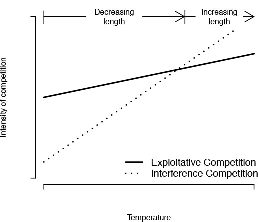
\includegraphics[width=0.5\textwidth]{1_CorpsDeThese/Resumes/Fig/FIP07b}
\caption[\lofimage{1_CorpsDeThese/Resumes/Fig/FIP07b}Importance relative
des différentes formes de compétitions]{Importance relative
des différentes formes de compétitions avec la température et leurs effets sur
la taille des adultes en condition de population.}
\label{fig:FIP7b}
\end{center}
\end{figure}

Les résultats présentés sur les populations HA trimodales montrent également que
la cohorte d'individus les plus grands imposent la densité et la taille de la
cohorte d'adultes plus petits. Ceci démontre encore une fois le rôle de la
compétition par interférence dans la régulation de nos populations, où un
adulte de grande taille reproduits les effets de densité dépendance produits par
quatre adultes de petite taille. La taille des plus grands adultes étant environ
deux fois supérieure à celle des adultes les plus petits dans les populations
trimodales, ce facteur d'environ 4 apporte par ailleurs un argument venant
appuyer l'hypothèse de la densité ressentie par les individus dépendante de la
longueur au carré dans le modèle présenté dans le Chapitre \ref{chap:amnat}, eq.
\refeq{eq_an2} page \pageref{eq_an2} (voir aussi Annexe \ref{An:AmNat}): $$
\eta(t,l)=\int_{l_b}^{l_m} \! C(l,\lambda)\cdot n(t,\lambda)\cdot\lambda^2\, \mathrm{d}\lambda $$.

Les mécanismes par les quels la température agit sur la compétition par
interférence ne sont cependant pas clairs. Nous avons montré dans le Chapitre
\ref{chap:sm} que les individus les plus grands empêchaient les plus petits
d'accéder à la ressource. Nous pensons que l'augmentation de la température, en
augmentant les taux métaboliques et l'activité augmentent à la fois la fréquence
à la quelle les collemboles sont en besoin de nourriture (2 fois par cycle de
vie, \citealp{palevody1974a}) alors que l'apport reste constant, et la fréquence
des interaction directes entre les individus, augmentant de ce fait l'intensité
de la compétition par interférence. 

La forme en U des normes de réactions de $GEBM$ pourrait donc être dues à
l'augmentation simultanée de la compétition par exploitation et par
interférence, mais avec des vitesses différentes (Figure \ref{fig:FIP7b}). En
dessous d'une température critique, bien qu'augmentant moins vite, la
compétition par exploitation reste la force régulatrice majeure de la dynamique
des populations, et l'augmentation de la température provoque alors une
diminution de la taille adulte qui tend vers la taille à maturité. Au-delà de la
température critique, la compétition par interférence devient dominante, et
l'augmentation de la température, en augmentant l'intensité de l'interférence,
favorise finalement des individus de grande taille. Dans ce cadre, l'existence
de populations trimodales à $21\degres$C, décrites dans les Chapitre précédents,
pourrait également être expliquée par des compétitions par exploitation et par
interférence relativement équilibrées qui ainsi permettrait l'émergence de
grands individus mais ne permettrait pas l'arrêt complet de la croissance des
juvéniles qui pourraient quand même maturer et s'arrêter de grandir à une taille
adulte intermédiaire. Ceci constitue donc une hypothèse complémentaire à
celle des conditions initiales pour l'apparition de ces populations trimodales.
En effet, bien qu'aillant des conditions initiales identiques, seules certaines
populations à $21\degres$C ont atteint des structures trimodales, jamais aux
autres températures. 

\section{En conclusion}

En mesurant des traits d'histoire de vie à la fois sur des individus isolés et
dans des populations, nous avons pu montrer que: (i) les effets de la densité
dépendance peuvent l'emporter sur les effets de la température attendus d'après
les mesures sur les individus isolés; et (ii) les effets de la densité
dépendance subissent eux-mêmes des changements liés aux conditions de
température. Ceci montre l'importance d'identifier clairement les différentes
composantes de la densité dépendance (compétition par exploitation ou
interférence par exemple) et leurs réponses à la température afin d'être capable
de prédire les réactions des populations aux changements de température en cours
et à venir. 







\partimage[width=\textwidth]{FigParts/writing3}
\part{Conclusion Générale}

\chapter{Dans une coque de noix}
\chaptermark{Dans une coque de noix}

\section{Principaux résultats de la thèse}

Au cours de cette thèse, nous avons exploré certains détails de la dynamique des
populations structurées, à la fois d'un point de vue expérimental que théorique.
Nous avons porté une attention toute particulière aux rôles que jouent les
interactions taille dépendantes entre individus dans l'établissement de ces
dynamiques, d'abord en observant des populations expérimentales de Collembole
\textit{Folsomia candida} sur le long terme pour en analyser les dynamiques en
fonction de leur structure en taille, puis en modélisant les interactions
tailles dépendantes entre individus dans un modèle physiologiquement structuré,
et enfin en manipulant la structure de la population et en observant les
comportement d'accès aux ressources. Nous nous sommes ensuite intéressé à
l'effet de l'environnement, via la température ambiante, sur ces interactions et
les répercussions sur la dynamique des populations.

Dans ce dernier chapitre, nous reviendrons sur les principaux enseignements que
l'on peut tirer de ces travaux par ses développements tant méthodologiques que
théoriques ou expérimentaux.

\subsection{Les développements méthodologiques}

J'ai choisi de revenir ici sur quelques développements méthodologiques réalisés
au cours de cette thèse car ils n'ont pas seulement occupé une grande partie de
mon travail, mais se sont également révélés indispensable au bon déroulement de
ces travaux. 

\subsubsection{Le phénotypage haut débit}

Le développement de la méthode d'analyse d'image pour le dénombrement et la
mesure de la structure des populations a été un élément clé qui a rendu possible
ce travail. Cette méthode de suivi des populations a été initialisées par
Thomas \textcites{tully2004a} au cours de sa thèse, puis reprise en développée
par François \textcites{mallard2013b} et moi même pendant plusieurs années avant
de faire l'objet d'un chapitre dans un ouvrage du CNRS
\autocites{le-galliard2012a} et d'une publication \autocites{mallard2013a}.

La méthode développé a notamment rendu possible la réplication des expériences
dans une mesure que l'on n'aura pas pu atteindre en dénombrant manuellement les
populations. C'est une méthode fiable qui permet à peu de frais d'accéder à la
structure en taille d'une population (et donc à la densité dans les différentes
classes de taille) en peu de temps et de façon très peu voir pas du tout
intrusive. 

Cette méthode a été développée et appliquée à des populations de collemboles,
mais est susceptible d'être facilement transposée à d'autres systèmes
expérimentaux comme cela a été décrit dans \textcites{mallard2013a}, ce qui lui
donne un grand intérêt pour l'écologie expérimentale et l'étude des traits
d'histoire de vie. 

\subsubsection{Diagrammes structure-temps}

Le travail présenté dans cette thèse n'aurait pas non plus été possible sans le
développement de la représentation graphique en diagrammes structure-temps et
des outils d'analyse graphique associés. En effet, cette technique simple de
représentation des données a permis de rendre cohérentes des données d'une
grande richesse dans les quelles il aurait été facile de se perdre. 

Nous pensons que l'application de cette méthode à des séries temporelles
structurées permettra de mettre en évidence des phénomènes qu'il était jusqu'à
présent difficile de décrire. Cette représentation rempli les critères
d'excellence des représentations graphiques en statistiques décrits par
\textcites{tufte1990a} en condensant une grande quantité d'information sur un
petit espace de représentation, sans déformer les données et en révélant
plusieurs niveaux de détails en une seul fois, des structures fines à la vue
d'ensemble \autocites{tufte2001a}. Avec le développement des méthodes
automatisées telles que celle présentée dans cette thèse \autocites[voir aussi
][]{le-galliard2012a} et la croissance toujours accélérée des bases de données
(``big data''), ce type de méthode devrait à l'avenir se démocratiser, autant en
écologie des populations que dans des domaines plus variés comme en
démographie humaine, en épidémiologie, dans les enquêtes d'opinion, d'usage,
\textit{etc}.

\subsection{Taille corporelle et populations structurées}

Au delà des apports méthodologiques, les travaux présentés dans cette thèse
répondent à des questions fondamentales en écologie des populations quant aux
rôle des interactions entre individus au sein d'une population dans la
régulation de sa structure et de sa dynamique, et à la place qu'occupe la taille
corporelle des individus dans la détermination de ces interactions.

\subsubsection{Taille corporelle et compétition par interférence}

Un premier résultat qui ressort de cet étude est l'importance de la différence
de taille corporelle dans la régulation de la dynamique de la structure en
taille de nos populations expérimentales. Nous avons pu montrer au cours des
différentes expériences menées et suivis de populations que la présence de
classes de tailles différentes en densité différentes avait un impact direct sur
la dynamique que l'on pouvait observer, tant à court terme qu'à long terme. La
présence d'individus de grande taille notamment s'est montré un critère
déterminant dans les dynamiques observées dans les différentes populations. 

En observant plusieurs populations dans les mêmes conditions, nous avons pu
montrer que les différentes structures en taille observées sont en nombre
limité, et peuvent être regroupées en quatre grande catégories. Ces catégories
de structures, que l'on a appelé structures types, se différencies par
l'abondance des juvéniles, la taille des adultes, et leur abondance. Une de ces
catégories est particulièrement remarquable par le fait qu'elle contient trois
modes séparés dans la distribution de la taille (les structures de types 4),
contrairement aux trois autres qui n'en contiennent que deux. Cette structure
type n'a par ailleurs été observée que chez un seul des deux clones étudiés, HA,
et cela quelque soit l'expérience menée. Le point commun entre les quatre
types de structure est la présence d'adultes à une taille corporelle stable
nettement supérieure à la taille à maturité, ce qui est contraire aux
prédictions des modèles de populations structurées régulées par compétition
intra-spécifique par exploitation.

L'observation des dynamiques de court terme dans ces populations a permis de
démontrer que ces adultes de taille relativement élevée jouaient un rôle
déterminant dans les dynamiques de la structure des populations. Leur
disparition progressive ou brutale coïncide de façon quasi systématique avec un
événement de recrutement de juvéniles dans les classes adultes. La perturbation
de la structure des populations dans une seconde expérience a permis de
renforcer le lien de causalité entre la présence des adultes et la croissance ou
non des juvéniles. En effet, retirer l'ensemble des adultes d'une de nos
populations de collemboles provoque un événement massif de recrutement alors que
ne retirer qu'une partie des adultes réduit
grandement le nombre de juvéniles qui parviennent à recruter. Lorsque plusieurs
classes de taille coexistent chez les adultes, le retrait des plus grands, même
moins nombreux, provoque un événement de recrutement plus important que le
retrait des plus petits. Retirer des individus de grande taille permet donc de
rendre la possibilité aux juvéniles de grandir et d'atteindre la maturité.

Cette domination des adultes sur la dynamique de la structure de nos populations
s'explique par la domination qu'ils exercent sur l'accès à la ressource fournie.
Cette hypothèse, issue de l'observation des séries temporelle de la structure
des populations, a été confirmée par l'observation des comportements d'accès à
la ressource et la mesure du biais de taille dans cet accès. Par ces mesures, on
a pu montrer une sur-représentation systématique des individus les plus grands
au contact ou aux abords de la pastille de ressource. Cette pastille de
ressource étant très localisée comparé à l'environnement de vie des Collemboles,
il est alors facile pour la minorité d'individus les plus grands de monopoliser
la ressource et d'en restreindre l'accès aux plus petits. Ces derniers ne
pouvant se nourrir ne peuvent alors pas se développer et restent dans un stade
juvénile jusqu'à ce que le nombre d'adultes diminue suffisamment pour que la
ressource deviennent à nouveau accessible. 

Ce comportement des individus les plus grands repoussant les plus petits aux
abords de la ressource et ses conséquences sur la dynamique de la structure
montrent l'existence d'une compétition par interférence, parfois de forte
intensité, dans nos populations de collemboles. Cette compétition par
interférence contre balance l'avantage énergétique que possèdent les petits
individus et permets ainsi au plus grands de survivre et de dominer la
population. 

\subsubsection{Compétition par interférence et dynamique des populations
structurées}

Nous avons donc montré le rôle de la compétition par interférence dans la
régulation de nos populations structurées en taille, et notamment comment elle
permettait la survie d'individus de grande taille, et parfois de géants très
longévives qui, même en petit nombre, dominent le reste de la population. 

Afin d'étudier plus avant les conséquence de l'existence d'une compétition
intra-spécifique par interférence sur la dynamique d'une population structurée,
nous avons repris le modèle classique de dynamiques de populations
physiologiquement structurées développé pour les Daphnies
\autocites{kooijman1984a}. Nous avons adapté ce modèle à notre système en le
paramétrant pour les collemboles, ce qui a été possible car le cycle de vie des
collemboles présente des similarités avec celui des daphnies dans le sens où les
collemboles ont une croissance continue et sont amétaboles, les juvéniles et les
adultes ayant la même apparence et partageant la même niche, ne se différenciant
que par la taille. Nous avons ensuite étendu le modèle pour y intégrer une
représentation des interactions directes entre individus dépendantes des
tailles respectives des adversaires. Nous avons alors été en mesure de modéliser
différents niveaux de compétition par interférence pour en observer les
conséquences sur la dynamique, comparé à un modèle avec de la
compétition par exploitation seule. Ce modèle présente l'avantage de rester
simple tout en regroupant les aspects principaux de la compétition par
interférence.

Nous avons montré avec ce modèle que la présence de la compétition par
interférence intra-spécifique pouvait avoir différentes conséquences en fonction
de son intensité. En l'absence d'interférence, la théorie existante sur les
modèles PSP décrit déjà les dynamiques prédites, et notamment la présence de
cycles de génération à faible mortalité, et l'effet stabilisant d'une forte
mortalité. Un premier résultat de ce modèle est l'effet stabilisant de la
compétition par interférence lorsqu'elle est à niveau intermédiaire. Si son
intensité est suffisante, la compétition par interférence vient contrebalancer
l'avantage des juvéniles par la compétition par exploitation, et produit ainsi
un effet similaire à l'augmentation de la mortalité basale en stabilisant les
cycles de génération. On obtient alors une structure de population stable
similaire à celle que l'on aurait sans interférence avec une forte mortalité
basale. 

L'augmentation de la compétition par interférence a aussi pour effet de faire
augmenter la capacité des individus les plus grands de la population à accéder à
la ressource. Lorsque cette capacité est suffisante, les individus, qui jusque
là arrêtaient de grandir à une taille proche de la taille à maturité, peuvent
alors reprendre leur croissance, et atteignent des tailles importantes, proche
de leur maximum physiologique possible. Il est intéressant de noter que cela se
produit aussi bien dans une dynamique stable que cyclique. Une fois dépassé le
seuil d'interférence permettant la survie des géants, ceux-ci seront toujours
présents dans les populations et les domineront, à moins que le niveau
d'interférence soit réduit. 

Enfin, à un niveau très élevé, la compétition par interférence donne un tel
avantage aux adultes de grande taille que la dynamique est déstabilisée dans un
nouveau type de cycles. Ces cycles sont également des
cycles de génération, mais de beaucoup plus grande amplitude et plus longue
période. De plus contrairement aux cycles observés en l'absence d'interférence,
ce sont cette fois les adultes qui dominent la dynamique et génèrent les cycles. 

La présence des individus de grande taille et les nouveaux cycles décrits
présentent des similarités avec d'autres phénomènes déjà étudiés dans les
populations structurées, notamment le cannibalisme, ou la compétition
différentielle entre adultes et juvéniles, mais apporte une nouvelle explication
aux dynamiques observées, parfois plus parcimonieuse que celles précédemment
proposées. Ce modèle de dynamique de populations structurées, régulées par la
compétition par interférence, permet donc de compléter les résultats
préexistants sur la compétition par exploitation et le cannibalisme comme
mécanisme régulateur des populations structurées. 

\subsection{Les effets de la température}

Au cours d'une dernière expérience, nous avons comparé des normes de réactions à
la température mesurées sur des individus isolés et dans des populations. Nous
avons pu montrer que les processus de régulation des populations tels que la
compétition par exploitation et par interférence, sont soumis aux
effets de l'environnement et notamment à la température ambiante à laquelle se
trouve la population. 

Nous avons montré en introduction que la température est un facteur abiotique
connu pour son impact sur les individus, les populations et les communautés.
Chez les organismes ectothermes, de part notamment son action sur les réactions
métaboliques, un changement de température affecte toute
la physiologie de l'individu, ce qui se répercute sur sa gestion de l'énergie,
son comportement, sa croissance et son investissement reproducteur. Ces
répercussions en cascades ont ensuite un impact fort sur la dynamique des
populations concernées, et qui elles-mêmes peuvent cascader sur la dynamique de
l'ensemble de la communauté. 

Plus précisément, nous avons montré dans le cas des collemboles que
l'augmentation de la température a un effet prévisible sur les individus isolés,
provoquant notamment une réduction de la taille asymptotique lors d'une
augmentation de température, conformément à la règle taille-température
\autocites{angilletta2009a}. En revanche, dans les populations, l'effet d'une
température plus élevée se retrouve confronté aux mécanismes de compétition
intra-spécifique, et le résultat sur la dynamique des populations et leurs
structures est moins facile à prévoir. Nous avons montré que dans une gamme
intermédiaire de réchauffement, la température provoque une diminution des taux
de croissance et des tailles corporelles adultes, mais dans une bien moindre
mesure que chez les individus isolés, les effets température sont en partie
tamponnés par les mécanismes de densité dépendance. 

De façon plus étonnante, dans des conditions de température élevée
($26\degres$C), nous avons montré que les tailles adultes ne suivent plus la
règle taille-température, même après avoir corrigé les mesures pour les effets
de la densité d'individus. Nous avons pu montré qu'à température élevée, il
devenait plus intéressant pour les individus d'investir dans la croissance et
d'atteindre des tailles supérieures, malgré les désavantages liés à la
température. Nous avons expliqué cela par une inversion des mécanismes de
régulation dans les populations entre compétition par exploitation et
compétition par interférence. Plus précisément, à température basse ou
intermédiaire, la compétition par exploitation pourrait avoir une plus grande
importance que la compétition par interférence dans la régulation des
populations. Nous proposons également que l'intesité des compétitions par
exploitation et interférence augmentent avec la température, mais que la
compétition par interférence augmente plus vite que la compétition par
exploitation, par exemple à cause de l'augmentation de l'activité et du besoin
en nourriture par unité de temps.
Ainsi, à partir d'une température critique, le désavantage d'une grande taille
lié à la température serait sur-compensé par l'avantage lié à la supériorité par
interférence. Malgré la température élevé, les individus de grande taille
gagnant un accès quasi-exclusif à la ressource deviennent alors dominant dans
les popualtions. 

En plus de son effet direct sur l'individu, la température a donc également un
effet sur les interactions entre les individus et modifie les rapports de force
compétitifs entre individus de petite et de grande taille. En modifiant ces
rapports de force, la température affect de la dynamique des populations non
seulement via ses effets sur les individus, mais également via ses effets sur
les mécanismes de compétition. 

\subsection{Compétition par interférence dans les populations
naturelles}

Les différents résultats de ces travaux montrent l'importance de considérer la
compétition par interférence dans la description, la compréhension et la
prédiction de la dynamiques des populations structurées en taille. La taille
individuelle est un élément structurant des populations extrêmement répandu dans
les populations naturelles. Il est donc important de pouvoir reconnaître dans
ces populations les effets de la compétition par interférence. Les données
expérimentales présentées dans ces travaux rendent assez facile la détection de
la compétition par interférence et l'analyse de son rôle dans la dynamique des
populations. Malheureusement, ces données très complètes sont difficiles voir
impossible à recueillir dans la nature. Il faut donc pouvoir se baser sur des
critères plus simples permettant de proposer la compétition par interférence
comme mécanisme participant à la régulation des populations. 

A cette fin, notre étude théorique nous a permis de proposer des critères de
recherche pour identifier le rôle de la compétition par interférence. Parmi ces
critères, l'émergence d'individus géants dans les populations. Ces individus ont
alors une durée de vie très longue comparée aux individus plus petits, et
peuvent dominer les dynamiques de populations. Bien que plusieurs mécanismes
puissent engendrer des géants (cannibalisme, niche écologique spécifique,
\ldots), la présence des géants un premier indice qui, associé aux critères
suivant, pointe vers la compétition par interférence.

Si les données recueillis le permettent, l'observation de courbes de croissance
en deux temps avec une stagnation (proche de la maturation) suivi d'une reprise
de croissance avant de converger vers une taille asymptotique élevée est
également une indice d'une compétition par interférence relativement intense. Ce
ralentissement de croissance (goulet d'étranglement de la croissance) provoque
alors des distributions de taille très asymétriques, fortement biaisées en
faveur des juvéniles dans le cas ou la population est stable. Si la structure de
la population est cyclique avec de longue périodes où la distribution est
multi-modale, cela indique un niveau élevé de compétition par interférence. 

Enfin, dans le cas où les données ne permettent pas l'observation détaillée des
courbes de croissance ou de la dynamique temporelle de la structure des
populations, la mesure du temps de génération comparée à la durée des
oscillations dans des populations périodiques (les oscillations sont mesurées en
comptant l'abondance totale de la population) permet également de proposer la
compétition par interférence comme mécanisme régulateur si le ratio des deux
grandeurs est entre 1 et 2. Ce dernier indice n'apporte pas la même fiabilité
que les critères précédent, mais peut permettre de poser l'hypothèse de la
compétition par interférence et de diriger les efforts de récolte des données
nécessaires à l'identification de son rôle, telles que les courbes de
croissances individuelles ou les données détaillées de structure au cours du
temps. 

\section{Hypothèses et limites}

Les résultats rapportés dans cette thèse sont issue de travaux expérimentaux et
théoriques. Comme tous les travaux de ce type, mes travaux comptent leur lot de
limitations et d'hypothèses sous-jacentes. Nous allons tenter ici de les
expliciter afin de montrer comment en tenir compte et éventuellement les
contourner ou les lever dans de futurs développements. 

\subsection{Approches expérimentales}

Les différentes expériences menées au cours de cette thèse on consister à suivre
des collemboles dans des conditions contrôlées. Les conditions d'élevages et de
mesure des populations entraînent quelques limitations qu'il est nécessaire de
mentionner.

\subsubsection{Conditions d'élevage}

Nos collemboles sont élevés dans des boites en plastiques de cylindriques de
$5.1cm$ de diamètre remplies d'un substrat de $3cm$ permettant de conserver
l'environnement d'élevage avec un taux de saturation en eau proche de $100\%$.
En effet, les collemboles sont extrêmement sensibles à la dessiccation. Ceci
constitue une première difficulté dans l'élevage et le suivi de populations de
collemboles. Cela nous oblige à surveiller régulièrement l'état de sécheresse
des boites d'élevage. En cas de boite sèche, la survie des collemboles n'excède
pas quelques jours, voir quelques heures à température élevée. Il est donc
essentiel de maintenir le taux d'humidité à son maximum pour éviter une
mortalité accrue des individus. 

Une autre limite intrinsèque aux conditions d'élevage des collemboles est liée à
l'humidité nécessaire à la survie des collemboles. En effet, ces conditions
d'élevages et l'apport régulier de ressources est propice au développement de
moisissures sur la pastille de ressources et le fond de la boite. Durant leur
développement, ces champignons produisent de longs filaments dans lesquels les
collemboles se retrouvent piégés, et qui occupent parfois l'intégralité de la
pastille de ressources. Les collemboles sont alors incapables de se nourrir,
même s'ils sont toujours libre. Ces champignons provoquent donc une mortalité
accrue chez les collemboles, soit en occupant la ressource, soit en piégeant les
individus. L'invasion d'une boite par des champignons touche principalement les
individus les plus petits qui sont plus facilement piégés dans les filaments. La
mortalité accrue est donc plus grande chez les juvéniles. De plus, une fois
installé, il est extrêmement difficile de se débarrasser des champignons. La
contamination d'une boite nécessite donc de transférer la population dans une
nouvelle boite d'élevage seine. Ceci peut alors entraîner des perturbations des
dynamiques, et est à l'origine de certains des événements catastrophiques
décrits dans le Chapitre \ref{chap:sp}. Une solution possible pour éviter la
contamination par les champignons peut être d'utiliser des pastilles de
nourritures traitées aux fongicides, mais l'innocuité de ce traitement sur les
collemboles n'est pas démontré, et nous avons choisi de ne pas l'utiliser dans
nos expériences. A la place, nous avons prêté une attention particulière à
l'état de nos boites d'élevage qui ont été nettoyées régulièrement. Malgré tout,
il a été impossible de prévenir toute contamination, et les populations
atteintes ont été transférées dans de nouvelles boites d'élevages dès que la
contamination a été constatée. 

\subsubsection{Protocole expérimental}

Les suivis de populations mis en place au cours de cette thèse reposent sur un
apport hebdomadaire de nourriture sous la forme d'une pastille de levure
dissoute dans de l'agar-agar. Sous cette forme, la pastille de nourriture occupe
très peu d'espace sur le fond de la boite d'élevage. Comme nous l'avons montré
dans cette thèse, la compétition pour l'accès à ces ressources est très forte et
le petit espace occupé par la pastille favorise les interactions et la
compétition par interférence. Ceci nous a permis de décrire les effets de ce
type de compétition sur les populations structurées, mais il est possible qu'une
partie des résultats décrits dans cette thèse soient la conséquence d'un niveau
extrême de compétition par interférence, du au format de ressources choisi. Bien
que cela ne remette pas en cause les résultats décrits, il est nécessaire de
tenir compte de ces conditions particulières dans l'analyse des résultats
obtenus. 

\subsubsection{Méthode de mesure}

Les populations suivis ont été dénombrées et leur structure en taille mesurées
par la méthode semi-automatique décrite dans le Chapitre \ref{chap:method}.
Comme nous l'avons décrit, cette méthode est particulièrement fiable pour des
populations de moins de 1000 individus. Les populations suivis au
cours des différentes expériences ont atteint et parfois dépassé ces densités.
il est alors possible que les mesures de la structure des populations soient
sous estimées. Plus précisément, lorsque la densité d'individus est très
élevées, les individus se touchent ou se superposent sur les photos utilisées
pour les dénombrements et les mesures de tailles. Ainsi, au lieu de compté
plusieurs individus de différentes tailles, l'algorithme d'analyse d'image
compte une seule particule de grande taille. Il est donc possible à très grande
densité que le nombre de juvénile soit sous estimé et le nombre de grands
adultes surestimé. Cependant, les comptages réguliers des boites et les
mesures moyennées sur plusieurs photos permettent d'augmenter la confiance dans
les mesures obtenues. De plus, malgré les incertitudes de mesure, la
représentation sous forme de diagramme structure-temps permet une représentation
de la dynamique de la structure qui rend apparent les dynamiques à courts termes
et les motifs sur le long terme en lissant en partie le bruit issue des données. 

\subsection{Hypothèses du modèle}

L'analyse théorique du rôle de l'interférence dans la dynamique des populations
structurées repose elle aussi sur un certain nombre d'hypothèse dont il faut
tenir compte. 

\subsubsection{Budget énergétique dynamique et allocation de l'énergie}

Une première hypothèse du modèle choisi repose sur la règle du
budget énergétique dynamiques. Cette règle suppose notamment que l'absorption
d'énergie se fait proportionnellement à la longueur au carré de l'individu alors
que sa consommation se fait proportionnellement à la longueur au cube. Les
règles du budget énergétique dynamique ont été établies d'après des travaux sur
divers organismes par \textcites{kooijman2000a}. Chez les organismes étudiés,
l'ingestion de nourriture se fait par une bouche dont la taille est généralement
proportionnelle à la longueur de l'individu. Le taux d'ingestion de la
nourriture (et donc de l'énergie) dépend alors de la surface de la bouche, qui
est donc proportionnelle à la longueur au carré de l'individu. Le taux de
consommation dépend quand à lui du nombre de cellules présentes dans
l'organisme, ce qui dépend du volume de l'individu, essentiellement
proportionnel à sa longueur au cube. Bien que ces relations soient très
générales, elles n'ont pas été vérifiées précisément chez les collemboles à
cause des difficultés que posent la mesure de l'ingestion et de la consommation
de l'énergie chez ces organismes. Cependant, la grande généralité de cette
hypothèse fait que l'on peut la supposer également chez le collembole sans trop
de doute sur sa véracité. 

Associé à ces hypothèse sur l'ingestion de l'énergie et sa consommation vient
l'hypothèse sur l'allocation du budget énergétique. Dans les travaux présentés
dans le Chapitre \ref{chap:amnat}, nous faisons l'hypothèse d'une allocation
suivant la règle dite du $\kappa$. Cette hypothèse se justifie notamment par le
fait que les collemboles se reproduisent tout au long de leur vie, même après
avoir stoppé leur croissance. Cependant, afin de vérifier que les résultats du
modèles ne sont pas directement la conséquence de cette règle d'allocation de
l'énergie, nous avons testé une seconde règle communément utilisée dans les
modèles de populations structurées, la règle dite de ``production nette''
(``net production model''). Sous cette nouvelle hypothèse, l'énergie est d'abord
allouée à la maintenance, et le reste (s'il y en a) est divisé entre croissance
et reproduction. Une conséquence immédiate de cette règle est que l'arrêt de la
croissance s'accompagne nécessairement d'un arrêt de la reproduction. Ceci est
donc très différent de la règle précédemment utilisée. L'analyse du modèle dans
le cadre du modèle de production nette est présentée dans les Supplementary
Materials de l'Annexe \ref{An:AmNat}, Section \ref{subsec:SupMat4}. Les
résultats qualitatifs en terme de type de dynamiques obtenues pour les
différentes valeurs d'interférence sont sensiblement identiques à ceux obtenus
pour la règle du $\kappa$. Ces résultats sont donc robustes et ne dépendent pas
de la façon dont l'énergie est répartie après acquisition. 

\subsubsection{Reproduction continue}

Le modèle utilisé est une extension du modèle de \textcites{kooijman1984a}. Ce
modèle a été développé pour les Daphnies. Nous l'avons transposé aux collemboles
après avoir vérifier les points essentiels assurant la validité du modèle
(voir Section \ref{subsec:SupMat1} des Supplementary
Materials de l'Annexe \ref{An:AmNat}). 

Le modèle utilisé fait l'hypothèse d'une reproduction continue des individus.
Cependant, les collemboles se reproduisent en produisant des pontes
relativement importantes tous les $10$ à $20$ jours suivant les conditions de
température et de densité des populations. A l'échelle des simulations
réalisées (plusieurs milliers de jours), cela peut être considéré comme
quasiment continue, cependant, il est possible que l'éclosion massive
d'individus au même moment entraîne des résultats différents d'une population ou
la reproduction est strictement continue. Nous pensons toutefois que cette
hypothèse de reproduction continue, par opposition à la reproduction saisonnière
de certains modèles de poissons, notamment intégrant du cannibalisme
\autocites{claessen2000a,claessen2004a}, reste valide pour les collemboles
compte tenu des échelles de temps mis en jeu et du nombre d'individus présents
dans les populations. En effet, même si chaque individus se reproduit de par des
pontes, la présence de nombreux adultes entraîne des éclosions quasi-continues
dans les populations. 

\subsubsection{Représentation de la compétition par interférence}

Afin d'implémenter la compétition par interférence dans le modèle, et parce que
les données correspondantes n'étaient pas disponibles, nous avons du faire une
première approximation et nous affranchir de la description explicite des
ressources et de leur consommation. Nous avons remplacé la dynamique de la
ressource par une dépendance directe de la population à sa propre densité (via
la fonction $\eta$). Cette approximation a été réalisée en supposant la
ressource à un état quasi stationnaire. Or, telle qu'elle est apportée dans les
populations expérimentales, la ressource n'est pas à un état quasi-stationnaire.
Il pourrait donc être intéressant de mesurer la consommation de la ressource
chez les collemboles afin de relaxer cette hypothèse et réintégrer la ressource
dans le modèle. L'apport ponctuel de ressource pourrait alors avoir un effet
important sur les dynamiques produites par le modèle. 

De plus, la compétition par interférence a été implémentée via la fonction de
compétition $C$ qui défini la supériorité d'un individu sur un autre en fonction
des tailles relatives des contestants. Cette fonction a été choisie affine de
fonction arbitraire avec une pente définie par l'intensité $I$ de la
compétition. Ce choix a été motivé par une volonté de simplicité de la
représentation. Mais ceci rend le modèle relativement théorique, et pas
forcément facilement applicable directement à des organismes. De plus, cette
représentation ne prends pas en compte la possible dépense d'énergie par les
contestant dans les interactions qui les opposent. Ainsi l'intérêt d'accéder à
la ressource pourrait être limité si la dépense d'énergie nécessaire au gain de
cet accès est supérieure à l'énergie gagnée. Ceci pourrait être pris en compte
en attribuant une forme plus complexe à la fonction de compétition qui
intégrerait par exemple une dépendance à la taille absolue en plus de celle à la
taille relative à l'autre contestant. En supposant qu'un individu plus grand
dépense moins d'énergie qu'un petit dans un conteste, ou que des individus
proches en taille dépensent plus d'énergie que des individus très éloignés, on
pourrait également obtenir des dynamiques prédites différentes suivant les
niveaux d'interférence. Cependant, cela complexifie la
modélisation, et nécessiterait de nouvelles mesures pour choisir et calibrer les
fonctions de compétition. Or ces mesures sont potentiellement difficiles
réalisées (notamment sur le collembole). De plus, malgré les différences
quantitatives, les résultats qualitatifs issus des simulations apportent des
éléments d'explication des dynamiques observées dans les suivis de populations.
Nous pensons donc que le modèle décrit ici fourni une représentation simple et
minimaliste, mais pertinente des mécanismes de base de la compétition par
interférence et de ses conséquences sur la dynamique des populations
structurées. 

\section{Perspectives futures}

Comme tout travail scientifiques, les réponses aux questions soulevées dans
cette thèse ne s'arrêtent pas aux conclusions exposées dans ce chapitre. Au
contraire, comme le montrent les limites présentées précédemment, beaucoup de
travail reste à faire pour comprendre pleinement les impacts de la compétition
par interférence sur la dynamique des populations. De même, des zones d'ombre
persistent quant à l'interaction de la compétition par interférence avec les
autres mécanismes de densité dépendance, et avec les facteurs environnementaux
comme la température, ou les facteurs climatiques plus large, la structuration
de l'habitat, et tout autre facteur susceptible d'influencer les individus et
les populations. Afin de répondre au critiques présentées précédemment et
d'approfondir la connaissance du rôle de la compétition par interférence dans la
dynamique des populations, nous proposons ici quelques pistes à la fois
expérimentales et théoriques pouvant apporter de nouveaux éclairages sur ces
questions.

\subsection{Développement expérimental}

\subsubsection{Limiter les risques de contamination}

D'un point de vu expérimental, nous avons vu que plusieurs problèmes peuvent se
poser en lien avec le système développé au cours de cette étude. Un premier
impératif pour garantir la validité des résultats expérimentaux obtenus est de
trouver une méthode pour limiter au maximum les risques de contamination par les
champignons. Une méthode permettant d'assainir les boites d'élevage consiste à
étaler un mélange d'argile et de charbon actif, inoffensif pour les collemboles,
sur le fond de la boite d'élevage. Cela fourni un meilleur environnement de vie
pour les individus tout en diminuant le risque de contamination. Cette méthode
ayant été développé après le lancement de nos suivis de populations, nous ne
l'avons pas utilisé dans nos expériences, mais elle a été testée et vérifiée par
François \textcites{mallard2013b} dans ses travaux de thèse et peut être
appliquée aux futures expériences. 

\subsubsection{Tester les nouvelles questions}

Les travaux menés au cours de cette thèse on soulevés de nouvelles questions, en
particulier concernant le lien entre le niveau de compétition par interférence
et les structures observées dans les dynamiques. Nous avons évoqué le fait que
le niveau élevé de compétition par interférence dans nos populations pouvait
être lié à la distribution très localisée de la ressource dans les boites
d'élevage. Un moyen de réduire le niveau de compétition par interférence et
ainsi de tester l'effet sur la dynamique de la structure des populations par
comparaison avec les résultats précédent, pourrait être de disperser la
nourriture apporter. Il s'agirait alors de fournir la même quantité de
nourriture mais occupant une surface plus grande sur le fond de la boite.
L'hypothèse est alors qu'en occupant une proportion plus grande de la surface de
la boite, l'accès aux pastilles de nourriture est plus facile pour l'ensemble
des individus, ce qui permettrait de diminuer les interactions pour y accéder,
tout en maintenant un niveau similaire de compétition par exploitation en
gardant la même quantité totale de nourriture. A l'inverse, un traitement ou la
nourriture serait apportée en plus petite quantité mais plusieurs fois par
semaine afin de conserver la même quantité hebdomadaire permettrait de renforcer
la compétition par interférence. En effet, les pastilles seraient alors encore
plus petites que dans les conditions déjà testée, et les combats pour y accéder
plus intenses. 

De telles expériences à $21\degres$C permettraient de comparer les dynamiques
obtenues avec celles présentées dans le Chapitre \ref{chap:sp}. Ces
comparaisons permettraient également de tester les prédictions du modèle
présenté dans le Chapitre \ref{chap:amnat}, et ainsi, en faisant varier le
niveau de compétition par interférence, vérifier si l'on peut obtenir
expérimentalement les différentes dynamiques produites par les simulations.
Cette validation expérimentale fournirait alors un argument en faveur de la
représentation simple de l'interférence proposée dans le modèle, et permettrait
également de tester les critères proposés pour reconnaître le rôle de
l'interférence. 

Étendues aux différentes températures testées dans le Chapitre \ref{chap:fip},
ces expériences permettraient de vérifier l'hypothèse proposée d'une bascule
entre domination de la compétition par exploitation et par interférence entre
$21$ et $26\degres$C. En effet, nous supposons que les tailles plus grandes
observées à $26\degres$C sont dues à une forte intensité de l'interférence qui
donne un avantage à des individus de grande taille malgré le désavantage causé
par une température élevée. En faisant varier les niveaux d'interférence à
aux différentes températures, nous pourrions vérifier s'il est possible
d'observer un avantage aux petites taille jusqu'à $26\degres$C en diminuant
l'interférence, ou au contraire, favoriser l'émergence de géant dès
$21\degres$C, voir avant. Ceci permettrait de valider notre hypothèse et de
confirmer les interactions entre processus démographiques et effets de la
température dans la régulation des populations.

Une autre piste envisageable dans pour étendre notre étude de la compétition
concerne l'impact de la température dans le cas d'un environnement changeant. On
pourrait modifier les températures d'élevage des collemboles avec différentes
fréquences et amplitude, et ainsi observer comment les variations de température
impactent la dynamique des populations par comparaison avec les résultats
obtenus dans le Chapitre \ref{chap:fip} pour des températures fixes. On peut par
exemple imaginer que l'effet de la compétition par interférence favorisant les
grandes tailles à haute température associé à celui de la température elle-même
pour des températures inférieurs provoque une synergie si les variations
conduisent la population dans les deux régions. Ainsi, les adultes pourraient
avoir des tailles encore supérieures à celles observées.

\subsection{Développement théorique}

\subsubsection{Relâcher les hypothèses du modèle}

La première hypothèse du modèle théorique décrite précédemment concerne le
budget énergétique dynamique et le rapport $l^2 / l^3$ dans la gestion de
l'énergie. Cette hypothèse est longuement discutée par \textcites{kooijman2000a}
et nous avons déjà expliqué pourquoi nous la pensons applicable à notre système.
De même, nous avons montré que le choix de la règle d'allocation de l'énergie
n'avait pas d'impact direct sur les dynamiques prédites par notre modèle.
Cependant, d'autres hypothèses du modèle mériteraient d'être relâchées afin
d'en rendre les prédictions plus générales. 

Au premier rang de celles-ci se trouve l'hypothèse d'état quasi-stationnaire des
ressources. A cause des difficultés que posent la mesure des taux de
consommation et d'utilisation individuels des ressources chez les collemboles,
nous nous sommes restreint à cette hypothèse. Cependant, un retour à un modèle
intégrant explicitement la dynamique de la ressource améliorerait
significativement le réalisme de ce modèle. De plus, il deviendrait du
même coup plus facile à étendre à d'autres organismes, ou à d'autres types de
ressources. Nous pourrions par exemple tester l'impact d'un forçage sur les
ressources sur la dynamique des populations structurées sous différents niveaux
de compétition par interférence. 

La seconde hypothèse majeure concerne la forme de la fonction de compétition.
Comme nous l'avons expliqué précédemment, une forme différente de la fonction de
compétition pourrait mener à des résultats très différents sur les dynamiques
des populations prédites, notamment en intégrant un coup énergétique à
l'interférence. Il serait donc nécessaire de tester de nouvelles descriptions
pour l'interférence, et ainsi de vérifier la généralité des résultats proposés
dans cette thèse. 

\subsubsection{Développer le modèle}

Au delà du simple relâchement des hypothèses fortes du modèle, plusieurs pistes
sont envisageables pour prolonger l'étude théorique des effets de l'interférence
sur la dynamique des populations structurées. Le premier développement à
envisager consisterait à ajouter une dépendance des traits physiologiques à la
température. L'addition de la température dans le modèle, en la calibrant sur
les normes de réactions mesurées chez les individus, permettant alors de tester
les hypothèses formulées à l'issue de l'expérience présentée dans le Chapitre
\ref{chap:fip}. Notamment, en jouant sur le niveau d'interférence à différentes
température, on pourrait alors vérifier s'il est possible de prédire avec ce
modèle les normes de réactions moyennes observées dans nos populations
expérimentales, et notamment si une compétition par interférence
suffisamment intense conduit à une augmentation de la taille adulte maximum à
haute température. 

L'intégration de la température dans le modèle permettrait également de tester
et établir des prédictions de dynamiques dans le cas de températures
fluctuantes. Les effets de la températures étant en interaction avec ceux des
processus démographiques, l'impact de changements plus ou moins réguliers de
l'environnement est alors difficile à prévoir. Ces prédictions pourraient être
testées et validées expérimentalement comme décrit précédemment. 

Enfin, d'autres pistes pour le développement du modèle pourraient par exemple
consister à ajouter de l'évolution, et de se placer dans le contexte de la
dynamique adaptative pour tenter de prédire le devenir de populations soumises à
un changement extérieur selon leur capacité à s'adapter, par exemple au niveau
du compromis entre croissance et reproduction. Les différentes stratégies
possibles pouvant être testées sur notre système expérimental grâce à la banque
de clone disponible dont les phénotypes ont été décrits et étudiés
\autocites{tully2004a}.

Dans un contexte de changement globaux, notamment anthropogéniques, les travaux
présentés dans cette thèse apportent de nouveaux éléments à la compréhension
détaillée de la dynamiques des populations structurées, et ouvrent de nouvelles
perspectives dans l'analyse et la prédiction des réponses de ces populations aux
changements à venir.
